% -*- Mode:TeX -*-

%% The documentclass options along with the pagestyle can be used to generate
%% a technical report, a draft copy, or a regular thesis.  You may need to
%% re-specify the pagestyle after you \include  cover.tex.  For more
%% information, see the first few lines of mitthesis.cls. 

%\documentclass[12pt,vi,twoside]{mitthesis}
%%
%%  If you want your thesis copyright to you instead of MIT, use the
%%  ``vi'' option, as above.
%%
%\documentclass[12pt,twoside,leftblank]{mitthesis}
%%
%% If you want blank pages before new chapters to be labelled ``This
%% Page Intentionally Left Blank'', use the ``leftblank'' option, as
%% above. 

\documentclass[12pt,vi,twoside,letterpaper]{mitthesis}
\usepackage{lgrind}
\usepackage{epsfig}
\usepackage{vmargin}
\usepackage{alltt}
\usepackage{verbatim}
\usepackage[figure]{algorithm2e}
\usepackage{multicol}

\pagestyle{plain}

\begin{document}

\setlength{\topmargin}{1in}
\setlength{\textheight}{9in}

%% Useful Thesis Submission Info: http://libraries.mit.edu/archives/thesis-specs/#geninfo
%%                            and http://www.eecs.mit.edu/ug/thesis-guide.html

% -*-latex-*-
% $Log: not supported by cvs2svn $
% Revision 1.7  2001/02/08 18:53:16  boojum
% changed some \newpages to \cleardoublepages
%
% Revision 1.6  1999/10/21 14:49:31  boojum
% changed comment referring to documentstyle
%
% Revision 1.5  1999/10/21 14:39:04  boojum
% *** empty log message ***
%
% Revision 1.4  1997/04/18  17:54:10  othomas
% added page numbers on abstract and cover, and made 1 abstract
% page the default rather than 2.  (anne hunter tells me this
% is the new institute standard.)
%
% Revision 1.4  1997/04/18  17:54:10  othomas
% added page numbers on abstract and cover, and made 1 abstract
% page the default rather than 2.  (anne hunter tells me this
% is the new institute standard.)
%
% Revision 1.3  93/05/17  17:06:29  starflt
% Added acknowledgements section (suggested by tompalka)
%
% Revision 1.2  92/04/22  13:13:13  epeisach
% Fixes for 1991 course 6 requirements
% Phrase "and to grant others the right to do so" has been added to
% permission clause
% Second copy of abstract is not counted as separate pages so numbering works
% out
%
% Revision 1.1  92/04/22  13:08:20  epeisach
\title{Language and Compiler Support for Stream Programs}

\author{William Thies}
\department{Department of Electrical Engineering and Computer Science}
% If the thesis is for two degrees simultaneously, list them both
% separated by \and like this:
% \degree{Doctor of Philosophy \and Master of Science}
%\degree{Doctor of Philosophy of Science in Computer Science and Engineering}
\degree{Doctor of Philosophy}
\degreemonth{September} \degreeyear{2008} \thesisdate{\today}

\prevdegrees{~ \\ 
Bachelor of Science, Computer Science and Engineering\\
Massachusetts Institute of Technology, 2001 \\
~ \\
Bachelor of Science, Mathematics\\
Massachusetts Institute of Technology, 2002 \\
~ \\
Master of Engineering, Computer Science and Engineering \\
Massachusetts Institute of Technology, 2002 \\
~ \\
}

%% By default, the thesis will be copyrighted to MIT.  If you need to copyright
%% the thesis to yourself, just specify the `vi' documentclass option.  If for
%% some reason you want to exactly specify the copyright notice text, you can
%% use the \copyrightnoticetext command.
%\copyrightnoticetext{\copyright IBM, 1990.  Do not open till Xmas.}

% If there is more than one supervisor, use the \supervisor command
% once for each.
\supervisor{Saman Amarasinghe}{Associate Professor}

% These are optional, and enabled with reader.sty
%\reader{Arvind}{Professor}
%\reader{Srini Devadas}{Professor}

% This is the department committee chairman, not the thesis committee
% chairman.  You should replace this with your Department's Committee
% Chairman.
\chairman{Terry P. Orlando}{Chair, Department Committee on Graduate Students}

% Make the titlepage based on the above information.  If you need
% something special and can't use the standard form, you can specify
% the exact text of the titlepage yourself.  Put it in a titlepage
% environment and leave blank lines where you want vertical space.
% The spaces will be adjusted to fill the entire page.  The dotted
% lines for the signatures are made with the \signature command.
\maketitle

% The abstractpage environment sets up everything on the page except
% the text itself.  The title and other header material are put at the
% top of the page, and the supervisors are listed at the bottom.  A
% new page is begun both before and after.  Of course, an abstract may
% be more than one page itself.  If you need more control over the
% format of the page, you can use the abstract environment, which puts
% the word "Abstract" at the beginning and single spaces its text.

%% You can either \input (*not* \include) your abstract file, or you can put
%% the text of the abstract directly between the \begin{abstractpage} and
%% \end{abstractpage} commands.

% First copy: start a new page, and save the page number.
\cleardoublepage
% Uncomment the next line if you do NOT want a page number on your
% abstract and acknowledgments pages.
% \pagestyle{empty}
\setcounter{savepage}{\thepage}
\begin{abstractpage}
As DSP programming is becoming more complex, there is an increasing
need for high-level abstractions that can be efficiently compiled.
Toward this end, we present a set of aggressive optimizations that
target linear sections of a stream program.  Our input language is
StreamIt, which represents programs as a hierarchical graph of
autonomous filters.  A filter is linear if each of its outputs can be
represented as an affine combination of its inputs.  Linear filters
are common in DSP applications; examples include FIR filters,
expanders, compressors, FFTs and DCTs.

We present a linear extraction analysis that automatically detects
linear filters based on the C-like code in their {\tt work} function.
Once linear filters are identified, we show how neighboring nodes can
be collapsed into a single linear representation, thereby eliminating
many redundant computations.  Also, we describe a method for
automatically translating linear nodes into the frequency domain,
thereby yielding algorithmic savings for convolutional filters.

We have completed a fully-automatic implementation of the above
techniques as part of the StreamIt compiler, and we demonstrate
performance improvements that average 400\% over our benchmark
applications.




\end{abstractpage}

% Additional copy: start a new page, and reset the page number.  This way,
% the second copy of the abstract is not counted as separate pages.
% Uncomment the next 6 lines if you need two copies of the abstract
% page.
% \setcounter{page}{\thesavepage}
% \begin{abstractpage}
% As DSP programming is becoming more complex, there is an increasing
need for high-level abstractions that can be efficiently compiled.
Toward this end, we present a set of aggressive optimizations that
target linear sections of a stream program.  Our input language is
StreamIt, which represents programs as a hierarchical graph of
autonomous filters.  A filter is linear if each of its outputs can be
represented as an affine combination of its inputs.  Linear filters
are common in DSP applications; examples include FIR filters,
expanders, compressors, FFTs and DCTs.

We present a linear extraction analysis that automatically detects
linear filters based on the C-like code in their {\tt work} function.
Once linear filters are identified, we show how neighboring nodes can
be collapsed into a single linear representation, thereby eliminating
many redundant computations.  Also, we describe a method for
automatically translating linear nodes into the frequency domain,
thereby yielding algorithmic savings for convolutional filters.

We have completed a fully-automatic implementation of the above
techniques as part of the StreamIt compiler, and we demonstrate
performance improvements that average 400\% over our benchmark
applications.




% \end{abstractpage}

\cleardoublepage

\newpage
~ \vspace{-3.7\baselineskip}\\
\enlargethispage{0.3\baselineskip}
\section*{Acknowledgments}

I would like to start by expressing my deepest gratitude to my
advisor, colleague and friend, Saman Amarasinghe.
%Saman's committment to me has been downright scary.
%Simply put, Saman has changed my life.
%Simply put, Saman has been the mentor of a lifetime.
From 4am phone calls in Boston to weeks of one-on-one time in Sri
Lanka and India, Saman invested {\it unfathomable} time and energy
into my development as a researcher and as a person.  His extreme
creativity, energy, and optimism (not to mention mad PowerPoint
skills!) have been a constant source of inspiration, and whenever I am
at my best, it is usually because I am asking myself: {\it What would
Saman do}?  Saman offered unprecedented freedom for me to pursue
diverse interests in graduate school -- including weeks at a time
working with other groups -- and served as a fierce champion on my
behalf in every possible way.  I will forever treasure our deep sense
of shared purpose and can only aspire to impact others as much as he
has impacted me.

%Like a Papa Bear, any arguments between the two of us would be 
%completely dwarfed by the fierce battles he would wage on my behalf.

\vspace{-8pt}\paragraph*{Contributors to this dissertation} Many
people made direct contributions to the content of this dissertation.
The StreamIt project was a fundamentally collaborative undertaking,
involving the extended efforts of over 27 people.  I feel very lucky
to have been part of such an insightful, dedicated, and fun team.
Section~\ref{sec:streamit-project} provides a technical overview of
the entire project, including the division of labor.  In what follows
I am listing only a subset of each person's actual contributions.
Michael Gordon, my kindred Ph.D. student throughout the entire
StreamIt project, led the development of the parallelization
algorithms (summarized in Chapter~4), the Raw backend and countless
other aspects of the compiler.  Rodric Rabbah championed the project
in many capacities, including contributions to cache optimizations
(summarized in Chapter~4), teleport messaging (Chapter~3), the MPEG2
benchmarks, an Eclipse interface, and the Cell backend.  Michal
Karczmarek was instrumental in the original language design (Chapter
2) and teleport messaging, and also implemented the StreamIt scheduler
and runtime library.  David Maze, Jasper Lin, and Allyn Dimock made
sweeping contributions to the compiler infrastructure; I will forever
admire their skills and tenacity in making everything work.

Central to the StreamIt project is an exceptional array of
M.Eng. students, who I feel very privileged to have interacted with
over the years.  Andrew Lamb, Sitij Agrawal, and Janis Sermulins led
the respective development of linear optimizations, linear statespace
optimizations, and cache optimizations (all summarized in Chapter~4).
Janis also implemented the cluster backend, with support for teleport
messaging (providing results for Chapter~3).  Matthew Drake
implemented the MPEG2 codec in StreamIt, while Jiawen Chen implemented
a flexible graphics pipeline and Basier Aziz implemented mosaic
imaging.  Daviz Zhang developed a lightweight streaming layer for the
Cell processor; Kimberly Kuo developed an Eclipse user interface for
StreamIt; Juan Reyes developed a graphical editor for stream graphs;
and Jeremy Wong modeled the scalability of stream programs.  Kunal
Agrawal investigated bit-level optimizations in StreamIt.  Ceryen Tan
is improving StreamIt's multicore backend.

The StreamIt project also benefited from an outstanding set of
undergraduate researchers, who taught me many things.  Ali Meli, Chris
Leger, Satish Ramaswamy, Matt Brown, and Shirley Fung made important
contributions to the StreamIt benchmark suite (detailed in Chapter~2).
Steve Hall integrated compressed-domain transformations into the
StreamIt compiler (providing results for Chapter~5).  Qiuyuan Li
worked on a StreamIt backends for Cell, while Phil Sung targeted a
GPU.

%Qiuyuan Li worked on a StreamIt backend for the Cell processor, while
%Phil Sung worked on a backend for graphics processors.

Individuals from other research groups also impacted the StreamIt
project.  Members of the Raw group offered incredible support for our
experiments, including Anant Agarwal, Michael Taylor, Walter Lee,
Jason Miller, Ian Bratt, Jonathan Eastep, David Wentzlaff, Ben
Greenwald, Hank Hoffmann, Paul Johnson, Jason Kim, Jim Psota, Nathan
Schnidman, and Matthew Frank.
%
\newpage
\enlargethispage{0.3\baselineskip}
%
~ \vspace{-1.3\baselineskip}\\
\noindent Hank Hoffmann, Nathan Schnidman, and Stephanie Seneff also
provided valuable expertise on designing and parallelizing signal
processing applications.  External contributors to the StreamIt
benchmark suite include Ola Johnsson, Mani Narayanan, Magnus
Stenemo, Jinwoo Suh, Zain ul-Abdin, and Amy Williams.  Fabrice
Rastello offered key insights for improving our cache optimizations.
Weng-Fai Wong offered guidance on several projects during his visit
to the group.  StreamIt also benefited immensely from regular and
insightful conversations with stakeholders from industry, including
Peter Mattson, Richard Lethin, John Chapin, Vanu Bose, and Andy Ong.

Outside of the StreamIt project, additional individuals made direct
contributions to this dissertation.  In developing our tool for
extracting stream parallelism (Chapter~6), I am indebted to Vikram
Chandrasekhar for months of tenacious hacking and to Stephen McCamant
for help with Valgrind.  I thank Jason Ansel, Chen Ding, Ronny
Krashinsky, Viktor Kuncak, and Alex Salcianu, who provided valuable
feedback on manuscripts that were incorporated into this dissertation.
I am also grateful to Arvind and Srini Devadas for serving on my
committee on very short notice, and to Marek Olszewski for serving as
my remote agent of thesis submission!

\vspace{-8pt}\paragraph*{The rest of the story} Throughout my life,
I have been extremely fortunate to have had an amazing set of
mentors who invested a lot of themselves in my personal growth.  I
thank Thomas ``Doc'' Arnold for taking an interest in a nerdy high
school kid, and for setting him loose with chemistry equipment in a
Norwegian glacier valley -- a tactic which cemented my interest in
science, especially the kind you can do while remaining dry.
%a tactic which ignited not only my interest in science, but also in
%girls.
I thank Scott Camazine for taking a chance on a high school programmer
in my first taste of academic research, an enriching experience which
%was not only enriching and fun, but also 
opened up many doors for me in the future.  I thank Vanessa Colella
and Mitchel Resnick for making my first UROP experience a very
special one, as evidenced by my subsequent addiction to the UROP
program.  I thank Andrew Begel for teaching me many things, not
least of which is by demonstration of his staggering commitment,
capacity, and all-around coolness in mentoring undergraduates.  I'm
especially grateful to Brian Silverman, a mentor and valued friend
whose unique perspectives on everything from Life in StarLogo to
life on Mars have impacted me more than he might know.  I thank
Markus Zahn for excellent advice and guidance, both as my
undergraduate advisor and UROP supervisor.  Finally, I'm very
grateful to Kath Knobe, who provided unparalleled mentorship during
my summers at Compaq and stimulated my first interest in compilers
research.

Graduate school brought a new set of mentors.  I learned a great
deal from authoring papers or proposals with Anant Agarwal, Srini
Devadas, Fredo Durand, Michael Ernst, Todd Thorsen, and
Fr\'{e}d\'{e}ric Vivien, each of whom exemplifies the role of a
faculty member in nurturing student talent.  I am also very grateful
to Srini Devadas, Martin Rinard, Michael Ernst, and Arvind for being
especially accessible as counselors, showing interest in my work and
well-being even in spite of very busy schedules.  I could not have
imagined a more supportive environment for graduate study.

I thank Charles Leiserson and Piotr Indyk for teaching me about
teaching itself.  I will always remember riding the T with Charles
when a car full of Red Sox fans asked him what he does for a living.
Imagining the impressive spectrum of possible replies, I should not
have been surprised when Charles said simply, ``I teach''.  Nothing
could be more true, and I feel very privileged to have been a TA in
his class.

I'd like to thank my collaborators on projects other than StreamIt,
for enabling fulfilling and fun pursuits outside 
% the work described in 
of this dissertation.  In the microfluidics lab, I thank
J.P. Urbanski for many late nights ``chilling at the lab'', his
euphemism for a recurring process whereby he manufactures chips and
I destroy them.  His knowledge, determination, and overall good
nature are truly inspiring.  I also learned a great deal from David
Craig, Mats Cooper, Todd Thorsen, and Jeremy Gunawardena, 
%
\newpage
\enlargethispage{0.5\baselineskip}
%
~ \vspace{-1.5\baselineskip}\\
\noindent who were extremely supportive of our foray into
microfluidics.  I thank Nada Amin for her insights, skills, and
drive in developing our CAD tool, and for being an absolute pleasure
to work with.

%In the microfluidics lab, I learned an immense amount from
%J.P. Urbanski, microfluidic wizard extraordinaire whose work ethic
%is as intense as it is understated -- never again will I think
%lightly of a late night ``chilling at the lab''.

I'm very thankful to my collaborators in applying technology towards
problems in socio-economic development, from whom I've drawn much
support.  First and foremost is Manish Bhardwaj, whose rare
combination of brilliance, determination, and selflessness has been
a deep inspiration to me.  I also thank Emma Brunskill, who has been
a tremendous collaborator on many fronts, as well as
%whose independence and resourcefulness are always humbling.  
%I'm very grateful to Emma Brunskill, Somani Patnaik, 
Sara Cinnamon, Goutam Reddy, Somani Patnaik and Pallavi Kaushik for
being incredibly talented, dedicated, and fun teammates.
%I thank the Venerable Tenzin Priyadarshi and Scott Kennedy for
%valuable support and guidance.
%
%Further in the past, 
I am very grateful to Libby Levison for involving me in my first
project at the intersection of technology and development, without
which I might have gone down a very different path.  I also thank
Samidh Chakrabarti for being a great officemate and friend, and my
first peer with whom I could investigate this space together.

I am indebted to the many students and staff who worked with me on
the TEK project, including Marjorie Cheng, Tazeen Mahtab, Genevieve
Cuevas, Damon Berry, Saad Shakhshir, Janelle Prevost, Hongfei Tian,
Mark Halsey, and Libby Levison.  I also thank Pratik Kotkar,
Jonathan Birnbaum, and Matt Aasted for their work on the Audio Wiki.
I would not have been able to accomplish nearly as much without the
%continuous 
insights, dedication, and hard work of all these individuals.

% leaving out sri lanka guys, since it's not released:
% - Thayaparan Kailainathan
% - Mahendrakumar Senthivel
% - Thayarupan Rajendram
%
% leaving out some TEK authors who I don't even know:
% - Alexandro Artola
% - Binh D. Vo
% - Yuliya Litvak
% - Sheldon Chan
% - Sid Henderson

Graduate school would be nothing if not for paper deadlines, and I
feel very lucky to have been down in the trenches with such bright,
dependable, and entertaining co-authors.  Of people not already cited
as such, I thank Marten van Dijk, Blaise Gassend, Andrew Lee, Charles
W. O'Donnell, Kari Pulli, Christopher Rhodes, Jeffrey Sheldon, David
Wentzlaff, Amy Williams, and Matthias Zwicker for some of the best
end-to-end research experiences I could imagine.

Many people made the office a very special place to be.  Mary McDavitt
is an amazing force for good, serving as my rock and foundation
throughout many administrative hurricanes; I can't thank her enough
for all of her help, advice, and good cheer over the years.  I'm also
very grateful to Shireen Yadollahpour, Cornelia Colyer, and Jennifer
Tucker, whose helpfulness I will never forget.  Special thanks to
Michael Vezza, system administrator extraordinaire, for his extreme
patience and helpfulness in tending to my every question, and fixing
everything that I broke.

I thank all the talented members of the Commit group, and especially
the Ph.D. students and staff -- Jason Ansel, Derek Bruening, Vikram
Chandrasekhar, Gleb Chuvpilo, Allyn Dimock, Michael Gordon, David
Maze, Michal Karczmarek, Sam Larsen, Marek Olszewski, Diego Puppin,
Rodric Rabbah, Mark Stephenson, Jean Yang, and Qin Zhao.  On top of
tolerating {\it way} more than their fair share of StreamIt talks,
they offered the best meeting, eating, and traveling company ever.  I
especially thank Michael Gordon, my officemate and trusted friend, for
making 32-G890 one of my favorite places -- I'm really going to miss
our conversations (and productive silences!)

I'd like to extend special thanks to those who supported me in my job
search last spring.  I feel very grateful for the thoughtful counsel
of dozens of people on the interview trail, and especially to a few
individuals (you know who you are) who spent many hours talking to me
and advocating on my behalf.  This meant a great deal to me.  I also
thank Kentaro Toyama and others at MSR India for being very flexible
with my start date, as the submission of this thesis was gradually
postponed!

I am extremely fortunate to have had a wonderful support network to
sustain me throughout graduate school.  To the handful of close
friends who joined me for food, walks around town, or kept in touch
from a distance: thank you for seeing me through the thick and thin.
I'd like to especially call out to David Wentzlaff, Kunal Agrawal,
Michael Gordon and Cat Biddle, who held front-row season tickets to my
little world and made it so much better by virtue of being there.

Finally, I would like to thank my amazingly loving and supportive
parents, who have always been 100\% behind me no matter where I am
in life.  I dedicate this thesis to them.

%% \clearpage
%% ~ \\ \vspace{1.1in} ~ \\
%% \begin{center}
%% {\bf \large Relation to Prior Publications}
%% \end{center}
\section*{Relation to Prior Publications}
This dissertation alternately extends and summarizes prior
publications by the author.  Chapters 1 and 2 are significantly more
detailed than prior descriptions of the StreamIt
language~\cite{thies-cc02,thies-can02,amarasinghe-ijpp05} and include
an in-depth study of the StreamIt benchmark suite that has yet to be
published elsewhere.  Chapter~3 subsumes the prior description of
teleport messaging~\cite{thies-ppopp05}, including key changes to the
semantics and the first uniprocessor scheduling algorithm.  Chapter~4
is a condensed summary of prior
publications~\cite{gordon-asplos02,lamb-pldi03,agrawal-cases05,sermulins-lctes05,gordon-asplos06},
though with new text that often improves the exposition.  Chapter~5
subsumes the prior report on compressed-domain
processing~\cite{thies07compression}, offering enhanced functionality,
performance, and readability.  Chapter~6 is very similar to a recent
publication~\cite{thies-micro07}.  Some aspects of the author's work
on StreamIt are not discussed in this
dissertation~\cite{karczmarek-lctes03,chen-graphics05}.

Independent publications by other members of the StreamIt group are
not covered in this
dissertation~\cite{kuo05,drake-ipdps06,zhang_lightweight_2007}.  In
particular, the case study of implementing MPEG2 in StreamIt provides
a nice example-driven exposition of the entire
language~\cite{drake-ipdps06}.

%\vspace{1in}
%\begin{center}
%{\bf \large Funding Acknowledgment}
%\end{center}
\section*{Funding Acknowledgment}
This work was funded in part by the National Science Foundation
(grants EIA-0071841, CNS-0305453, ACI-0325297), DARPA (grants
F29601-01-2-0166, F29601-03-2-0065), the DARPA HPCS program, the MIT
Oxygen Alliance, the Gigascale Systems Research Center, Nokia, and a
Siebel Scholarship.
\clearpage

% NOT ACKNOWLEDGING:
%
% - Meha Senthil?
%
% StreamIt:
% - Vijay Saraswat
% - Ryan Newton
% - Ken Steele provided an IPAQ for some of the experiments in Chapter~4.
%
% Teaching:
% - David Liben Nowell
% 
% Microfluidics:
% - natalie andrew
%
% IIH:
% - Seema Kacker
% - Sourav Dey
% - Ajit Dash
% - Alex Krull
% - Oliver Venn
% - Jessica Leon
% - Nikhil Nadkarni
% - Catherine Dunn
%
% Job search:
% - christos kozyrakis
% - ras bodik
% - monica lam
% - stuart russel
% - krste asanovic
% - martin rinard
% - mark horowitz
%
% - arvind
% - eric grimson
%
% FRIENDS
% Grad school:
% - Gleb Chuvpilo
% - Satvika Chalasani
% - Gireeja Ranade
% - Jamie Stevenson
%
% - Maya Shivakumar
% - J.P. Urbanski
% - Amy Williams
% - Peter Mattson
% - Maya Rao
%
% Roommates:
% - Johnny Chen
% - Jacob Myerson
% - Cody Nave
% - Kenneth Lu
% - Rachel West
%
% College:
% - Minhaj Siddiqui
% - Xuemin Chi
% - Alice Tsay
% - Elaine Wan 
% - Manu Sridharan
% - Josh Sussan
% - Julie Hong
% - Robyn Treadwell
%
% High-school:
% - Austin Mandryk
% - Ankit Chander
% - Jerusha Achterberg
%
% All these details:
%
% I am indebted to many additional students and collaborators who
% helped to pursue goals at the intersection of technology and
% development in my graduate school career.
%
% For external contributions to TEK, from Elsevier I thank Ammy
% Votglander, Craig Scott, Jeremy Alder, Spencer de Groot, and
% Christian Pruvost; from First Mile Solutions, I thank Rich
% Fletcher, Amir Alexander Hasson, and Olufemi Omojola; from the
% People's First Network, I thank David Leeming.  
%
% At Innovators In Health, I thank Manish Bhardwaj, Sara Cinnamon,
% Goutam Reddy, Emma Brunskill, Somani Patnaik, Pallavi Kaushik,
% Seema Kacker, Sourav Dey, Ajit Dash, Alex Krull, Oliver Venn,
% Jessica Leon, Nikhil Nadkarni, and Catherine Dunn.  
%
% I also thank Rich Fletcher, Michael Gordon, Jonathan Jackson,
% Jhonatan Rotenberg, Luis Sarmenta, Ammy Votglander for many
% conversations benefiting this research.  I would not have been
% able to accomplish nearly as much without the steadfast
% dedication and help of all of these individuals.


%%%%%%%%%%%%%%%%%%%%%%%%%%%%%%%%%%%%%%%%%%%%%%%%%%%%%%%%%%%%%%%%%%%%%%
% -*-latex-*-

\pagestyle{plain}

  % -*- Mode:TeX -*-
%% This file simply contains the commands that actually generate the table of
%% contents and lists of figures and tables.  You can omit any or all of
%% these files by simply taking out the appropriate command.  For more
%% information on these files, see appendix C.3.3 of the LaTeX manual. 
\tableofcontents
\newpage
\listoffigures
% \newpage
% \listoftables



\section{Introduction}

Applications that are structured around some notion of a ``stream''
are becoming increasingly important and widespread.  There is evidence
that streaming media applications are already consuming most of the
cycles on consumer machines \cite{Rix98}, and their use is continuing
to grow.  In the embedded domain, applications for hand-held
computers, cell phones, and DSP's are centered around a stream of
voice or video data.  The stream abstraction is also fundamental to
high-performance applications such as intelligent software routers,
cell phone base stations, and HDTV editing consoles.

Despite the prevalence of these applications, there is surprisingly
little language and compiler support for practical, large-scale stream
programming.  Of course, the notion of a stream as a programming
abstraction has been around for decades \cite{SICP}, and a number of
special-purpose stream languages have been designed (see
\cite{survey97} for a review).  Many of these languages and
representations are elegant and theoretically sound, but they often
lack features and are too inflexible to support straightforward
development of modern stream applications, or their implementations
are too inefficient to use in practice.  Consequently, most
programmers turn to general-purpose languages such as C or C++ to
implement stream programs.

There are two reasons that general-purpose languages are inadequate for
stream programming.  Firstly, they are a mismatch for the application
domain.  That is, they do not provide a natural or intuitive
representation of streams, thereby having a negative effect on
readability, robustness, and programmer productivity.  Moreover, because
the widespread parallelism and regular communication patterns of data
streams are left implicit in general-purpose languages, compilers are
not stream-conscious and do not perform stream-specific optimizations.
As a result, performance-critical loops are often hand-coded in a
low-level assembly language and must be re-implemented for each target
architecture.  This practice is labor-intensive, error-prone, and very
costly.

Secondly, general-purpose languages are a mismatch for the emerging
class of grid-based architectures \cite{smartmemories,rawshort,trips} that
are especially well-suited for stream processing.  Perhaps the primary
appeal of C is that it provides a ``common machine language'' for
von-Neumann architectures.  That is, it abstracts away the
idiosyncratic differences between machines, but encapsulates their
common properties: a single program counter, arithmetic operations,
and a monolithic memory.  However, for grid-based architectures, the
von-Neumann model no longer holds, as there are multiple instruction
streams and distributed memory banks.  Thus, C no longer serves as a
common machine language--in fact, it provides the wrong abstraction
for the underlying hardware, and architecture-specific directives are
often needed to obtain reasonable performance.  Again, this greatly
complicates the job of the programmer and hampers portability.

StreamIt is a language and compiler specifically designed for modern
stream programming.  The StreamIt language has two goals: first, to
provide high-level stream abstractions that improve programmer
productivity and program robustness within the streaming domain, and
second, to serve as a common machine language for grid-based
processors.  At the same time, the StreamIt compiler aims to perform
stream-specific optimizations to achieve the performance of an expert
programmer.

This paper motivates, describes, and justifies the high-level language
features of StreamIt, version 1.0.  The major limitation of StreamIt
1.0 is that all flow rates in the streams must be static; applications
such as compression that have dynamically varying flow rates will be
the subject of future work.  A large set of applications can be
implemented with static rates, and while dynamic rates will require a
different runtime model, it will still be essential to fully analyse
and optimize static sub-sections in order to obtain high performance.

The paper is organized as follows. In Section {\ref{sec:domain}}, we
characterize the domain of streaming programs that motivates the
design of StreamIt, and in Section~\ref{sec:overview} we describe the
language features in detail.  We present an in-depth example of a
software radio in Section~\ref{sec:example}, preliminary results in
Section~\ref{sec:results}, related work in Section~\ref{sec:related},
and conclusions in Section~\ref{sec:conc}.


\chapter{The MPEG-2 Motion Picture Compression Standard}
\label{chapter:mpeg2}

MPEG-2~\cite{MPEG2} is a popular coding standard for
digital video. 
The scheme is a subset of both the DVD-Video~\cite{Taylor:1999:SDV} 
standard for storing movies, and the Digital Video Broadcasting 
specifications for transmitting HDTV and SDTV~\cite{DVB}. The scheme is
used by a wide variety of multimedia applications and appliances such
as the Tivo Digital Video Recorder~\cite{tivo}, and the DirecTV satellite broadcast
service~\cite{directv}. 

The amount of compression possible depends on the video data. 
Common compression ratios range
from 10:1 to 100:1. For example, HDTV, with a resolution of 1280x720
pixels and a streaming rate of 59.94 frames per second, has an
uncompressed data rate of 1.33 gigabits per second. It is compressed at
an average rate of 66:1, reducing the required streaming rate to
20 megabits per second~\cite{imagevidstandards}.

\begin{figure}
  \begin{center}
    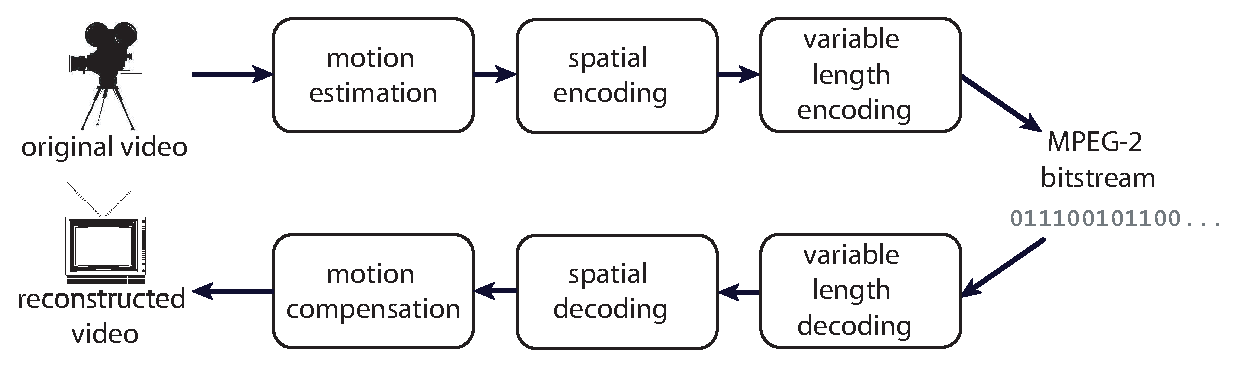
\includegraphics[scale=0.7, angle=0]{./mpeg2_overview.eps}
    \caption{High level view of MPEG-2 decoding and encoding.}
    \label{fig:mpeg2_overview}
  \end{center}
\end{figure}

The MPEG-2 specification contains three types of compression:
variable length coding, spatial coding, and motion prediction.
Figure~\ref{fig:mpeg2_overview} shows a high level overview
of the decoding and encoding process. 
For a complete description of the MPEG-2 data format and coding
scheme one should refer to
the official MPEG-2 standard~\cite{MPEG2}. However, this chapter
contains an abbreviated explanation of the 
standard targeted to a reader lacking prior knowledge of image or video
compression algorithms. The explanation focusses on the 
variable length coding in the parser, 
the functionality needed for spatial coding and decoding,
and the motion prediction components. Iwata et al. estimate that each of these three 
components constitutes a roughly equal portion of the work needed for 
decoding~\cite{iwata98coarse}. Encoding is similar, although
motion estimation constitutes a larger computational effort than
the decoder's motion compensation.

This chapter begins with an enumeration 
of the compression types found in MPEG-2.
It then describes picture organization and the temporal and spatial
transformations that provide compression. 
This is followed by a description of video
organization and finally a list of optional MPEG-2 format extensions.

\section{Compression Techniques}
MPEG-2 uses both {\it lossy} and {\it lossless} compression. 
Lossless compression eliminates redundant information from a signal while allowing
for an exact reconstruction. 
Lossy compression permanently eliminates information from a picture based on
a human perception model. Lossy compression removes details that a casual
observer is likely to miss. A lossy compression is irreversible,
and a lossy decompression process only approximately reconstructs the original
signal. MPEG-2 uses the following compression techniques:

\begin{itemize}
  \item \textbf{Huffman Compression} (\textit{lossless}) 
Huffman compression~\cite{Huffman52} is a form of entropy 
coding. It compresses a signal using variable length codes to efficiently 
represent commonly occurring subpatterns in the signal.
  \item \textbf{Color Channel Downsampling} (\textit{lossy})  
Humans are much better at discerning changes in {\it luminance}, 
than changes in {\it chrominance}. Luminance, or brightness, is a 
measure of color intensity. Chrominance is a measure of color hue.
Pictures are separated into one luminance and two chrominance channels, 
called the \textit{YCbCr} color space. The chrominance channels are
typically downsampled horizontally and vertically. 
  \item \textbf{Frequency Quantization} (\textit{lossy}) 
An image can be expressed as a linear combination of 
horizontal and vertical frequencies.
Humans are much more sensitive
to low frequency image components, such as a blue sky, than to high frequency image components,
such as a plaid shirt. Unless a high frequency component has 
a strong presence in an image, it can be discarded.
Frequencies which must be coded are stored 
approximately (by rounding) rather
than encoded precisely. This approximation process is called
\textbf{quantization}. How the different horizontal and vertical
frequencies are quantized is determined by empirical data
on human perception.
  \item \textbf{Motion Prediction} (\textit{lossless}) 
Frames of a video
contain a great deal of temporal redundancy because much of a
scene is duplicated between sequential frames. Motion estimation is used to
produce motion predictions with respect to one or more reference frames.
Predictions indicate what any given frame should look like. For similar frames, 
only the motion estimate and any error between the predicted values and the
actual values must be encoded.
  \item \textbf{Difference Coding} (\textit{lossless})  
Over any given region in an image the average color value is likely to be
similar or identical to the average color in surrounding regions.
Thus the average colors of regions are coded differentially with respect
to their neighbors. Motion information at neighboring regions is also likely
to be similar or identical and is therefore coded 
differentially with respect to motion at neighboring regions.
\end{itemize}

\section{Picture Organization} 
\label{section:picture_decomp}

\begin{figure}
  \begin{center}
    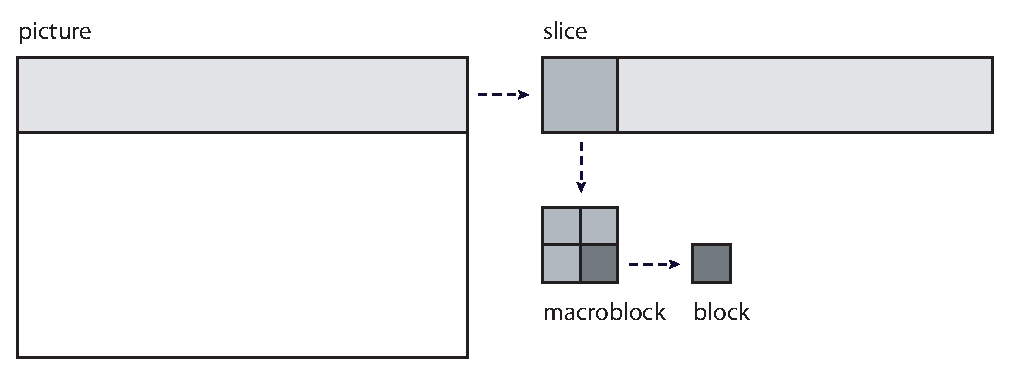
\includegraphics[scale=0.8, angle=0]{./picture_structure.eps}
    \caption{MPEG-2 picture subcomposition.}
    \label{fig:picture_structure}
  \end{center}
\end{figure}

Figure~\ref{fig:picture_structure} shows how the MPEG-2 standard
organizes pictures. Each picture breaks into 
16x16 groups of pixels called \textbf{macroblocks}. 
Adjacent sequences of macroblocks
are contained in a structure called a \textbf{slice}.
Pictures and macroblocks are defined in the
YCbCr color space, and the first step of encoding is
converting the picture into this color representation.

A macroblock is itself composed of 8x8 subpixel 
\textbf{blocks}. There are always
exactly 4 luminance blocks that form a 2x2 array to cover the
macroblock. Because of human insensitivity to chrominance information, each of the two
chrominance channels may be downsampled. 

The type of downsampling in an MPEG-2 stream is called its
\textbf{chroma format}. The two most common chroma formats
are shown in Figure~\ref{fig:chroma_format}. The more common of the two 
is the 4:2:0 format.
This format specifies that each chrominance channel in a macroblock be represented
by a single block, horizontally and vertically
downsampling a macroblock from 16x16 to 8x8 subpixels. 
A 4:2:0 macroblock therefore contains a total of 6 blocks.
An alternate format is 4:2:2. 
The 4:2:2 format uses two blocks for each chrominance 
channel, horizontally downsampling each macroblock from 16x16 to 
8x16 subpixels. 
A 4:2:2 macroblock therefore contains a total of 8 blocks.
A 4:4:4 chroma format also exists but is not commonly used, and specifies 
no color channel downsampling, and uses 4 blocks to 
represent each color channel in a macroblock. 

\begin{figure}
  \begin{center}
    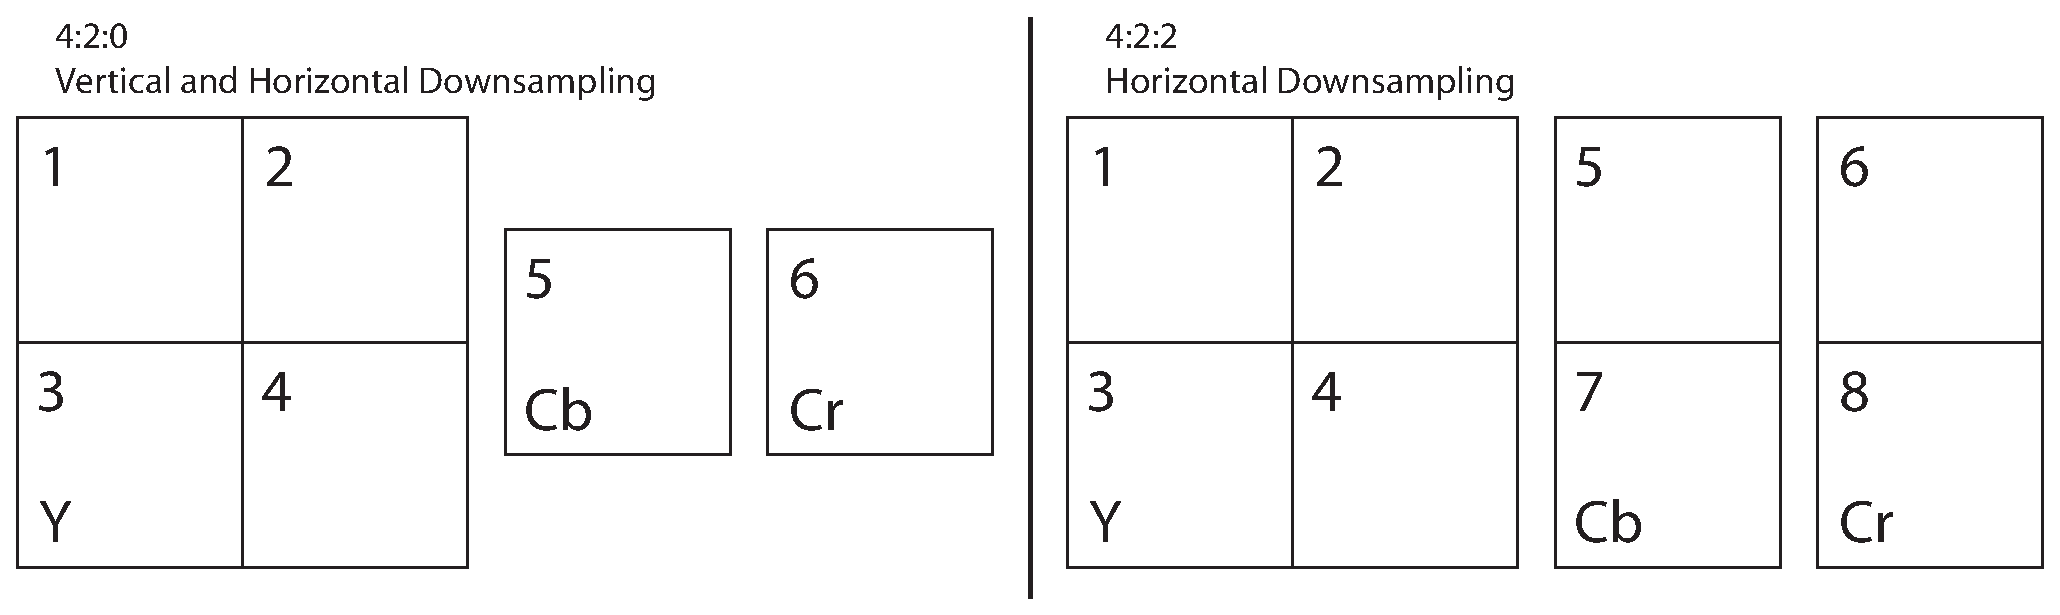
\includegraphics[scale=0.4, angle=0]{./chroma_formats.eps}
    \caption{Commonly used chroma formats.}
    \label{fig:chroma_format}
  \end{center}
\end{figure}

\section{Temporal Compression}

Temporal compression in MPEG-2 is achieved via motion prediction,
which detects and eliminates similarities between macroblocks across
pictures. For any given macroblock $M$, a motion estimator forms a prediction: a \textbf{motion
vector} that contains the horizontal and vertical displacement of that 
macroblock from the most similar macroblock-sized area in one or more reference pictures.
The matching macroblock
is removed (subtracted) from $M$ on a pixel by pixel
basis. The
result is a residual \textbf{predictive coded (P)} macroblock. The residual 
macroblock contains the difference between the motion predicted values for
the macroblock and the macroblock's actual values. A P macroblock
always uses forward motion prediction, meaning that the reference frame
precedes it temporally. (See Section~\ref{subsection:pic_org} for more details on
picture referencing and organization.) Figure~\ref{fig:motion_estimation_forward} illustrates
forward motion estimation.

\begin{figure}[h]
  \begin{center}
    \includegraphics[scale=0.5, angle=0]{./motion_estimation_forward_vectorized.eps}
    \caption{Eliminating temporal redundancy through forward motion estimation.}
    \label{fig:motion_estimation_forward}
  \end{center}
\end{figure}

Macroblocks encoded without the use of motion
prediction are \textbf{intra coded (I)} macroblocks. 
In addition to the forward motion 
prediction used by P macroblocks, it is possible to 
encode new macroblocks using motion
estimation from both temporally previous and subsequent pictures. Such macroblocks
are \textbf{bidirectionally predictive coded (B)} macroblocks, and they exploit a
greater amount of temporal locality. A B macroblock may contain two motion vectors, 
referencing both previous and subsequent pictures; in this case, the 
motion prediction
is an unweighted average of the forward and backward predictions. 
Figure~\ref{fig:motion_estimation_back}
illustrates backward motion estimation.

\begin{figure}[h]
  \begin{center}
    \includegraphics[scale=0.5, angle=0]{./motion_estimation_back_vectorized.eps}
    \caption{Eliminating temporal redundancy through backward motion estimation.}
    \label{fig:motion_estimation_back}
  \end{center}
\end{figure}

All blocks in macroblocks, whether intra coded or residually encoded, undergo 
spatial compression.
Except for the first macroblock in a slice, 
motion vectors are compressed by coding them differentially with respect to the 
motion vectors in the previously decoded 
macroblock\footnote{A second exception is for the first set of
motion vectors following an intra coded macroblock. These vectors 
must always be fully coded because intra coded macroblocks have no motion
vectors.}.

\section{Spatial Compression}
\label{sec:MPEGspatial}

Each block undergoes a two-dimensional \textbf{Discrete Cosine Transform} (DCT),
which is a frequency transform that separates the block into components
with varying visual importance. As shown in Figure~\ref{fig:dct}, 
the DCT takes one 8x8 block as input and produces a 
transformed 8x8 block of frequency coefficients as output. 
Horizontal frequency increases towards the right of the block and
vertical frequency increases towards the bottom of the block.
The upper left corner of the block contains the lowest frequencies
and the lower right corner contains the highest frequencies.

\begin{figure}
  \begin{center}
    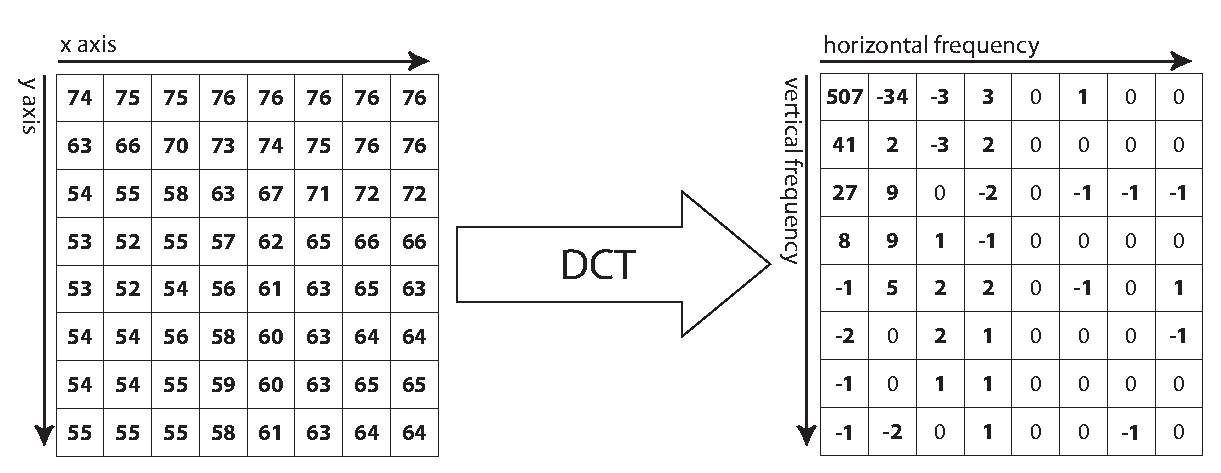
\includegraphics[scale=0.6, angle=0]{./dct.eps}
    \caption{Sample input and output for a discrete cosine transform.}
    \label{fig:dct}
  \end{center}
\end{figure}

The DCT by itself is lossless\footnote{I ignore a possible loss of 
precision, an issue addressed by the MPEG-2 specification and explained
subsequently in Section~\ref{subsection:extra_decoder}}
but enables the quantization of blocks according to a 
\textbf{quantization table} of \textbf{quantization values}, 
also in the frequency domain. The quantization table reflects
a human's relative abilities to discern different frequency
components of an image. 
The quantization table itself may contain any values and can be
specified in the MPEG-2 bitstream, although usually one 
of several standard tables is used.
Each value in a frequency-transformed
block is divided by the corresponding quantization value, with
any remainder thrown away. An example block quantization appears
in Figure~\ref{fig:quantize}\footnote{The quantization process is
technically more complicated than the math I have just described,
although the description is conceptually accurate. The output block
in the figure is accurately quantized, but cannot be arrived at by
the division process I just described.}.
A small error may be introduced
to individual frequency components and most low energy frequency components
are simply reduced to $0$. This stage introduces much of the lossy 
compression in MPEG-2 coding. 

\begin{figure}[h]
  \begin{center}
    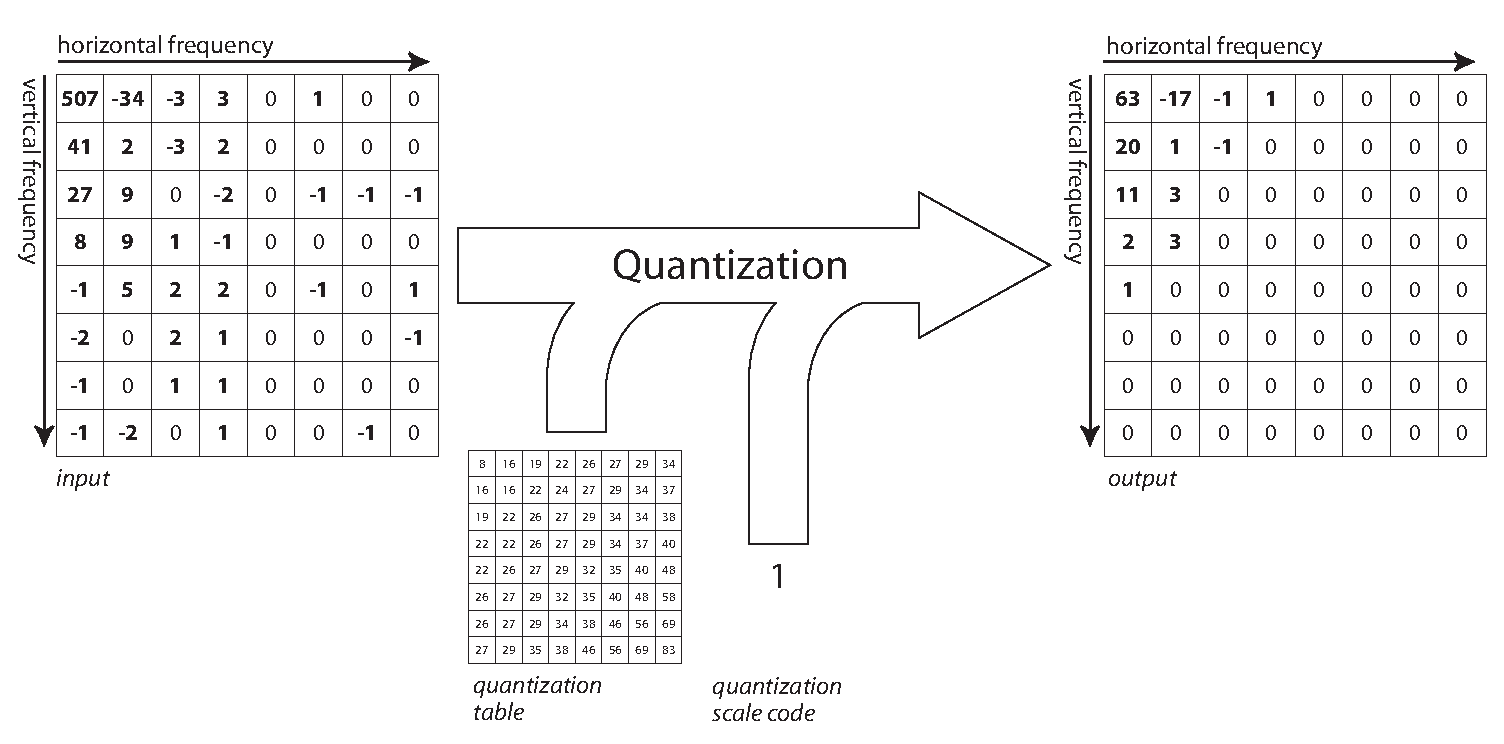
\includegraphics[scale=0.6, angle=0]{./quantization_example2.eps}
    \caption{Example block quantization.}
    \label{fig:quantize}
  \end{center}
\end{figure}

MPEG-2 uses two quantization tables. One table is used for all 
intra coded blocks and the other for residually coded blocks. 
At irregular intervals, an MPEG-2 bitstream indicates a 
\textbf{quantization scale code} which provides an additional 
scaling factor that affects all frequencies in a block. 
One can adjust the desired compression level and
control the video bitrate (bits per second)
by tuning the quantization scale code between macroblocks. 
In an encoder this control 
is typically realized using feedback about the final entropy coded 
output bitrate earlier in the quantization stage.

The upper left value in the frequency transformed block contains the
\textbf{DC coefficient}, which
is the coefficient corresponding to the zero frequency
in both the horizontal and vertical dimensions. Less formally,
this is the average color of the block. 
MPEG-2 differentially encodes the DC block value for 
intra coded blocks. 
The first DC coefficient in the first block in a slice is fully
encoded and all subsequent DC coefficients in a slice are 
differentially coded. Note that the differential coding
semantics for DC coefficients and motion vectors guarantee that
macroblocks in different slices are coded
independently from each other.

After quantization a block is \textbf{zigzag} ordered. 
Zigzag ordering sorts a
block's values from lowest to highest frequency. Since
low-frequency components are more likely to have non-zero 
values following quantization, zigzag ordering consolidates 
non-zero block coefficients together at the beginning of the block. 
The zigzag order commonly used by MPEG-2 is shown in Figure~\ref{fig:zigzag_order}

\begin{figure}
  \begin{center}
    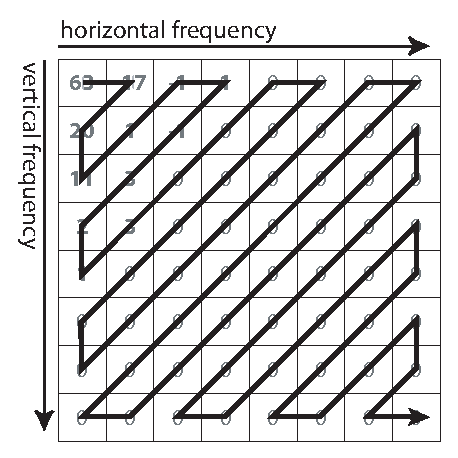
\includegraphics[scale=0.6, angle=0]{./zigzag_order.eps}
    \caption{Zigzag ordering of frequency coefficients from low to high.}
    \label{fig:zigzag_order}
  \end{center}
\end{figure}

The zigzag ordered data is then Huffman compressed using 
a set of predefined Huffman tables defined in the MPEG-2 
specification. Picture metadata, such as the picture type, changes
to the quantization scale code, and motion vectors,
are also Huffman encoded and interleaved in the bitstream.

\section{Required Block Decoding Components}
\label{subsection:extra_decoder}

Data transformation pairs such as a DCT and an inverse DCT (IDCT), may accidentally
introduce loss of data precision, 
due to hardware architecture and algorithm differences 
in a decoder and encoder.
While such imprecisions are tiny, the use of temporal compression
means that small imprecisions accumulate and magnify over the course
of several motion predicted pictures and quickly become noticeable.
For this reason the MPEG-2 specification places specific functional constraints on
mathematical operations in MPEG-2 codecs: 

\begin{itemize}
\item The frequency coefficients emitted from the inverse quantization stage must be saturated within predefined levels.
\item The low-order bit of the highest frequency value in a block is used as a parity bit on the value of the block. In the encoder this bit is set between the DCT and quantization. In the decoder the bit is checked between the saturated inverse quantization and the IDCT. This setting and checking of the bit is called \textbf{mismatch control}.
\item The output of the IDCT is saturated within predefined levels.  
\end{itemize}

\section{Video Organization}

\label{subsection:pic_org}

Just as macroblocks have an associated I, P, or B type, 
pictures also have an associated type, used to 
limit the kinds of macroblocks that they may contain. I pictures 
contain only I macroblocks, P pictures contain I or P macroblocks, 
and B pictures may contain I, P, or B macroblocks. Only I and P 
pictures are used as references for motion prediction and
all I and P pictures are automatically considered references. 
B pictures are never used as references. 

The highest level of organization in an MPEG-2 data stream
is the \textbf{Group of Pictures} (GOP), which 
contains all the information needed to reconstruct a temporally continuous sequence of
video. GOPs consist of I, P, and B pictures.
A typical I:P:B picture ratio in a GOP is 1:3:8, and a typical
picture pattern is a repetition of the following logical sequence,
where the subscripts denote the temporal ordering of the pictures in the video:
\begin{center}
I$_1$~B$_2$~B$_3$~P$_4$~B$_5$~B$_6$~P$_7$~B$_8$~B$_9$~P$_{10}$~B$_{11}$~B$_{12}$~I$_{13}$~$\cdot$~$\cdot$~$\cdot$
\end{center}

Any backwards motion vector in a picture refers to the immediately preceding
reference picture. Likewise, any forward motion vector refers to the subsequent
reference picture. To simplify the decoding process, pictures are not ordered
temporally in the data stream, but rather in the order that they are needed for decoding:
P pictures are always coded with respect to the previous
reference picture and B pictures are always coded with respect to the previous two
reference pictures. Thus, the picture pattern previously described is ordered
in the MPEG-2 data stream as:
\begin{center}
I$_1$~P$_4$~B$_2$~B$_3$~P$_7$~B$_5$~B$_6$~P$_{10}$~B$_8$~B$_9$~I$_{13}$~B$_{11}$~B$_{12}$~$\cdot$~$\cdot$~$\cdot$
\end{center}

\section{Additional MPEG-2 Features}
\label{additional:mpeg}
Because MPEG-2 targets a wide range of devices, the specification is complicated by additional features that make decoding any given video possible on a range of architectures. The following features are mentioned for the sake of completeness, but are excluded from the StreamIt MPEG-2 codec implementations. These features constitute alternative data formats, rather than compression or algorithmic enhancements, and are suitable for exclusion in research-oriented MPEG-2 implementations.

\begin{itemize}
\item \textbf{Interlacing} is a legacy television format needed to support many analog output devices. An interlaced frame contains only half of the original picture data, leaving out alternating horizontal lines. Sequential frames alternate between encoding even and odd scan lines. The alternative to interlacing, which fully encodes each picture, is called \textbf{progressive scan}. 
\item The MPEG-2 bitstream can contain \textbf{layers} which contain alternate encodings of the same picture. A motivating example for this feature is the DVD format, which typically encodes an interlaced version of a movie in the primary layer, and an interlaced version containing the alternate scan lines in a secondary layer. Devices that output interlaced pictures can ignore the secondary layer and devices that output progressive pictures can combine the two layers to produce the complete video.
\item \textbf{Concealment motion vectors} indicate motion estimates for intra-coded macroblocks. These concealment motion vectors are only used to form a macroblock prediction if bitstream errors prevent correct recovery of blocks contained in the macroblock. This plays an important role in the decoding of broadcast MPEG-2 streams such as satellite or HDTV, where transport errors are likely to occur.
\end{itemize}

\section{Related Work}
\label{sec:related}

Software pipelining for clustered vliws \cite{qian02}.

The Imagine stream processor~\cite{rixner98bandwidthefficient}
supports a time-multiplexed execution model.  The architecture
contains 48 parallel ALU's organized into 6 VLIW clusters.  The
programming model requires the programmer to write computation filters
in Kernel-C and stitch them together using Stream-C.  Because the
execution unit is data-parallel, the compiler uses time multiplexing
to execute a single filter at a time across all of the parallel
clusters.  While this provides perfect load balancing and high
arithmetic utilization when there is abundant data parallelism, it
suffers when a filter has retained state or data-dependences between
iterations.  Moreover, architectures based solely on
time-multiplexing do not scale spatially, as there are global wires
orchestrating the parallel execution units. 

Previous work in compiling StreamIt to Raw has taken a purely space
multiplexed approach~\cite{streamit-asplos}.  In this model, a single
filter was mapped to each execution tile.  To support applications
with more filters than execution tiles, a partitioning algorithm was
employed to adjust the granularity of the graph by fusing adjacent
filters into one.

Previous work in scheduling computation graphs to parallel targets
have focused on dynamic techniques \cite{SDFSched, SDFSched2,
may87communicating, DAGSched}. In general, multiple graph nodes are
{\it clustered} onto a single computational node and scheduled
dynamically.  

Our work, unlike most previous work in this field,
models link contention and topography.  Furthermore, StreamIt graphs
are implicitly formed of loops so we can apply loop scheduling
techniques such as software pipelining to build our schedules.

%The problem of instruction scheduling for MIMD and VLIW architectures
%is similar to the problem tackled by the space-time compiler.  ILP
%compilers for clustered VLIW architectures~\cite{Bulldog, Multiflow}
%are decomposed into stages that are analogous to the stages of the
%SpaceTime compiler.  These compilers must partition or cluster
%instructions, assign instructions to processors, and then schedule the
%instructions.  

Previous work on software pipelining has focused on scheduling machine
instructions in a loop \cite{lam-softpipe, rau-softpipe} to a
uniprocessor target.  The algorithms devised must account for tight
resource constraints and complex instruction dependences.  Our
software-pipelining problem is much less constrained, a traditional
modulo scheduling algorithm can not effectively take advantage of this
flexibility.  Previous work on ILP scheduling for the Raw
architectures ~\cite{lee98spacetime} also bears similarity.  However,
these compilers schedule graphs of fine-grained instructions. The
partitioning and scheduling heuristics are mindful of a different set
of constraints including different types of dynamism and less regular
communication patterns as compared to StreamIt graphs.

As far as we know, we are the first to apply loop-level scheduling
techniques to the problem of scheduling coarse-grained task graphs.

% \cite{cheops-thesis}
%   http://web.media.mit.edu/~kung/publication/thesis.pdf
%
% other possible things to cite:
%  http://portal.acm.org/citation.cfm?id=801721&dl=ACM&coll=portal
%  http://www.csrl.unt.edu/~kavi/Research/ica3pp156.pdf
%  http://cdmetcalf.home.comcast.net/papers/cop/node1.html#SECTION00010000000000000000

\Section{MPEG Decoder in StreamIt}

The MPEG decoder pipeline is shown in
Figure~\ref{fig:dec-with-code}. The stream graph is shown on the
left. The StreamIt code is shown on the right, and it is correlated
with the stream block level diagram.

%% The decoder accepts a compressed bit stream as input, and produces the
%% decoded video stream as output.
The computation is encapsulated in three main components:
the parser (line 8), the block and motion vector decoder (lines 9-22),
and the motion compensator (lines 23-32).
The parser is responsible for parsing the MPEG-2 bit stream and
performing Huffman and variable run-length decoding (VLD). The output
of the VLD is an interleaved stream of quantized macroblocks encoded
in the frequency-domain, and offset-encoded motion vectors. The VLD
outputs $\texttt{N}\times\texttt{B}$ data elements for each
macroblock, followed by \texttt{V} data elements that encode its
motion vector. The actual value of \texttt{N} depends on the chroma
format. In a 4:2:0 chroma format regime, $\texttt{N}=6$ since each
macroblock consists of four 8x8 subpixel blocks for the luminance
channel, and two 8x8 subpixel blocks for the two chrominance
channels. Therefore, the VLD outputs a total of six 8x8 blocks, or 384
subpixels per macroblock. However, the total number of macroblocks
that are output by the parser is dependent on the number of frames in
the input encoded video. As a result, the VLD has a variable I/O
rate. The VLD filter is the only variable rate filter in the decoder
pipeline.

The VLD output is segregated into two homogeneous streams by a
roundrobin splitter (line 10). The first stream undergoes inverse
transformations (lines 11-16), while the second is decoded to produce
absolute motion vectors (lines 17-20). As is evident from the computation
graph, the two streams are decoded in parallel, and then merged (line
21) prior to the motion compensation stage of the pipeline.

The inverse transformations map each 8x8 block from the frequency
domain back to the spatial domain. Each block is reordered
(line 12), and then inversely quantized (line 13). This is followed by
an inverse DCT and a bounded saturation filter (lines 14-15). The set
of transformations is grouped into a pipeline whose input
and output types are automatically inferred by the compiler. Each of
the filters in this pipeline operate on 8x8 blocks. The code that is
shown does not take advantage of data level parallelism between
blocks. It is rather straightforward however to expose this
parallelism if it is desirable. For example, in this case a splitjoin
can replicate the inverse transformation pipeline $N$ times:
\begin{center}
  \begin{scriptsize}
    \begin{verbatim}
      add splitjoin {
        split roundrobin(B);
        for (int i = 0; i < N; i++) 
        // add pipeline
        join roundrobin(B);
      }
    \end{verbatim}
  \end{scriptsize}
\end{center}
\vspace{-12pt}
A stream-aware compiler can also automatically adjust the execution
granularity as necessary~\cite{gordon02asplos}, since data-parallel streams
can be easily identified as those that are stateless (i.e., do not
carry mutable state from one iteration to the next).

The third stage of the decoding pipeline performs the motion
compensation (lines 23-32) to recover predictively coded
macroblocks. The motion compensation filter uses the motion vectors to
find a corresponding macroblock in a previously decoded reference
picture. The reference macroblock is added to the current macroblock
to recover the original picture data. If the current macroblock is
part of an I or P picture, then the decoder stores it for use as a
future reference picture.

In the compensation stage, there are three parallel streams.  The
first handles the luminance color channel (Y), and the other two
handle the chrominance channels (Cb and Cr). The roundrobin splitter
(line 24) distributes the macroblocks according to the chroma
format. Since the luminance channel is not downsampled during the
encoding process, the splitter dispatches four 8x8 blocks at a time to
the Y motion compensator. The chrominance channels are typically
downsampled by a factor of 4, and hence one 8x8 block is streamed to
each of the Cb and Cr pipelines, which upsample (line 29) the results
of the motion compensator to generate the full 16x16 macroblock.  The
upsampling is a linear interpolation of the surrounding pixels.
The joiner (line 31) assembles the pictures from each of the color
channels, one pixel at a time.  The output is then readied for display
(lines 33 and 34) by organizing the pictures in accord with their
temporal order, and performing color space conversion to the RGB (red,
green, blue) color model. Note that these two filters each consume
$3\times\texttt{W}\times\texttt{H}$ subpixels per picture. This is
three times the pixel resolution of the decoded image since there is
one pixel generated from each of the three channel decoders. The final
output of the decoder is $\texttt{W}\times\texttt{H}$ pixels.  In
contrast to the filters for motion compensation and inverse transformation,
whose I/O rates are statically resolved at compile time, the picture 
reordering and color space conversion have I/O rates that are
parameterized on initialization time constants, namely the pixel
resolution of the pictures.

%% The MPEG-2 decoder in StreamIt is a fully portable implementation in
%% that the application is not architecture dependent. The implementation
%% naturally exposes the pipeline parallelism that exists throughout the
%% decoder, as well as the data level parallelism inherent to the inverse
%% transformations and motion compensation.  

The decoder implementation was carried out by one student programmer
with no prior understanding of MPEG. The development spanned eight
weeks from specification~\cite{MPEG2} to the first fully functional
MPEG decoder. The StreamIt code is nearly 3,165 lines of code with 48
static streams. The bit stream parser is the largest single filter,
consisting of 775 lines of code. The 48 static streams compile to
2,150 instantiated filters\footnote{A  {\it static stream} is a unique
code block, which may have multiple instantiations. For instance,
\texttt{MotionCompensation()} is a single filter with three
instantiations.} at a picture resolution of 352x240. By way of
comparison, the reference C implementation~\cite{reference-mpeg-c} is
6,835 lines of code\footnote{Line counts were generated using  the
\texttt{SLOCcount} tool. It strips whitespace and comments.}.  A line
count comparison is not an accurate measure of programmability, since
our StreamIt decoder implements only a subset of several stream types
supported by MPEG.  Our decoder does provide full support for the
range of different compression techniques used within MPEG, but
supports only a subset of the possible display modes (i.e. interlaced
versus progressive output).  However, these alternate display formats
represent minor conceptual changes and should therefore affect small
portions of the StreamIt code. This is demonstrated in
Section~\ref{section:chroma} with an example that illustrates how to
support multiple chrominance formats.

The reference C implementation intermingles parsing, decoding, and
motion compensation, making it difficult to clearly follow the code,
and hindering a better comparison. The C code also relies on global
variables to communicate values, such as quantization coefficients,
from the parser to the relevant code regions. In StreamIt, such
communication is relegated to teleport messaging (lines 13, 25, 28, and
33, and illustrated with dotted lines in
Figure~\ref{fig:dec-with-code}). For instance, the parser (VLD)
generates a message whenever the picture or macroblock type
changes. The motion compensation filters receive this information via
their dedicated portal (line 28), determine how to process the current
picture, and decide whether they needs to store the picture for future
reference. Note however that while there are multiple motion compensators
subscribed to the same portal, they each receive the same message with
respect to their local execution.
The picture reordering filter receives a similar message
(via portal on line 33), and uses the information to determine the
correct temporal order of pictures. The inverse transformation
pipeline listens to its portal (line 13) to determine the algebraic
manipulation required to perform the inverse quantization of the input
macroblock. Teleport messaging 
%% proves as a natural mechanism because
%% the macroblock type and picture type information changes infrequently
%% and irregularly, compared to the regular flow of data in the
%% application. Moreover, by 
exposes the flow of messages to the compiler, and allows for large
scale reordering or parallelization of the application without a
heroic dependence analysis. It also provides a mechanism to easily
introduce dynamic behavior into an otherwise static processing pipeline.

%% \begin{figure*}[b]
%%   \centerline{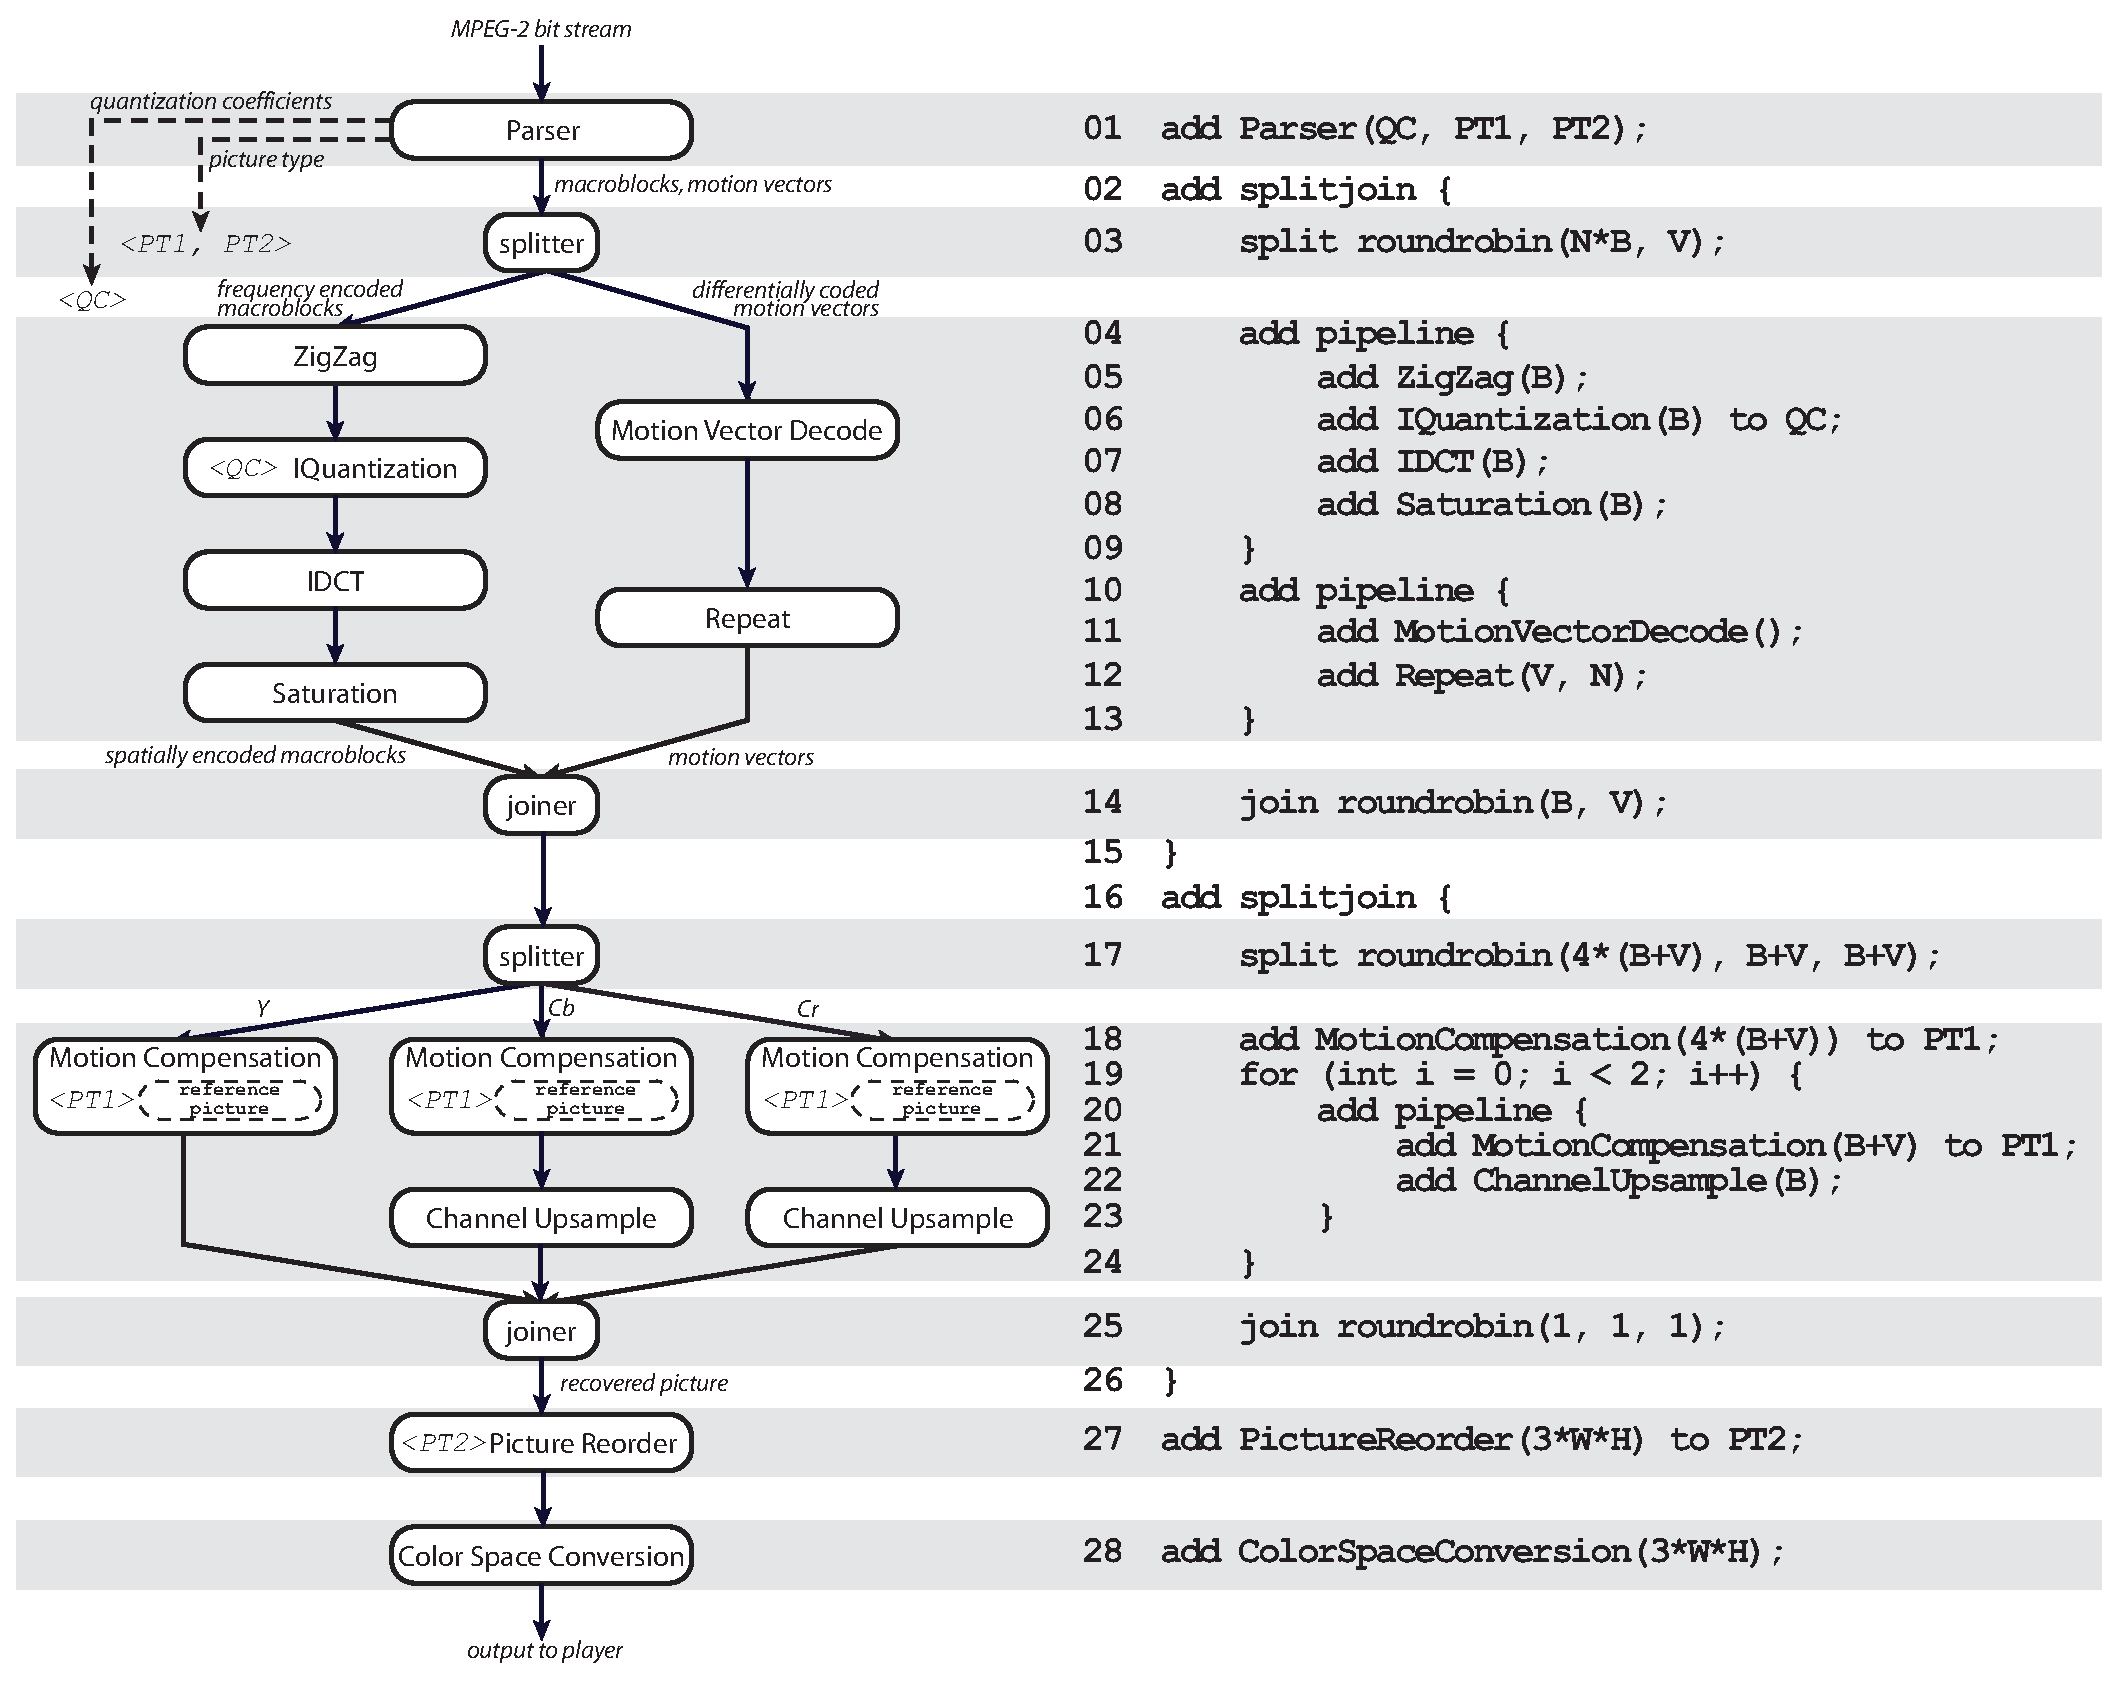
\epsfig{file=decoder_with_code.eps,width=\textwidth}}
%%   \caption{MPEG-2 decoder block diagram and corresponding StreamIt code.}
%%   \label{fig:dec-with-code}
%% \end{figure*}

In StreamIt, all of the processing is encapsulated hierarchically into
single-input, single-output streams with well-defined modular
interfaces. This facilitates development and boosts programmer
productivity, as components can be debugged and verified as standalone
components. The modularity also promotes reuse. For example, the
zig-zag descrambler and inverse DCT can be used as-is in a JPEG decoder.

%%%%
\begin{figure}[h]
  \begin{minipage}{\textwidth}
  \vspace{-1.1in}
  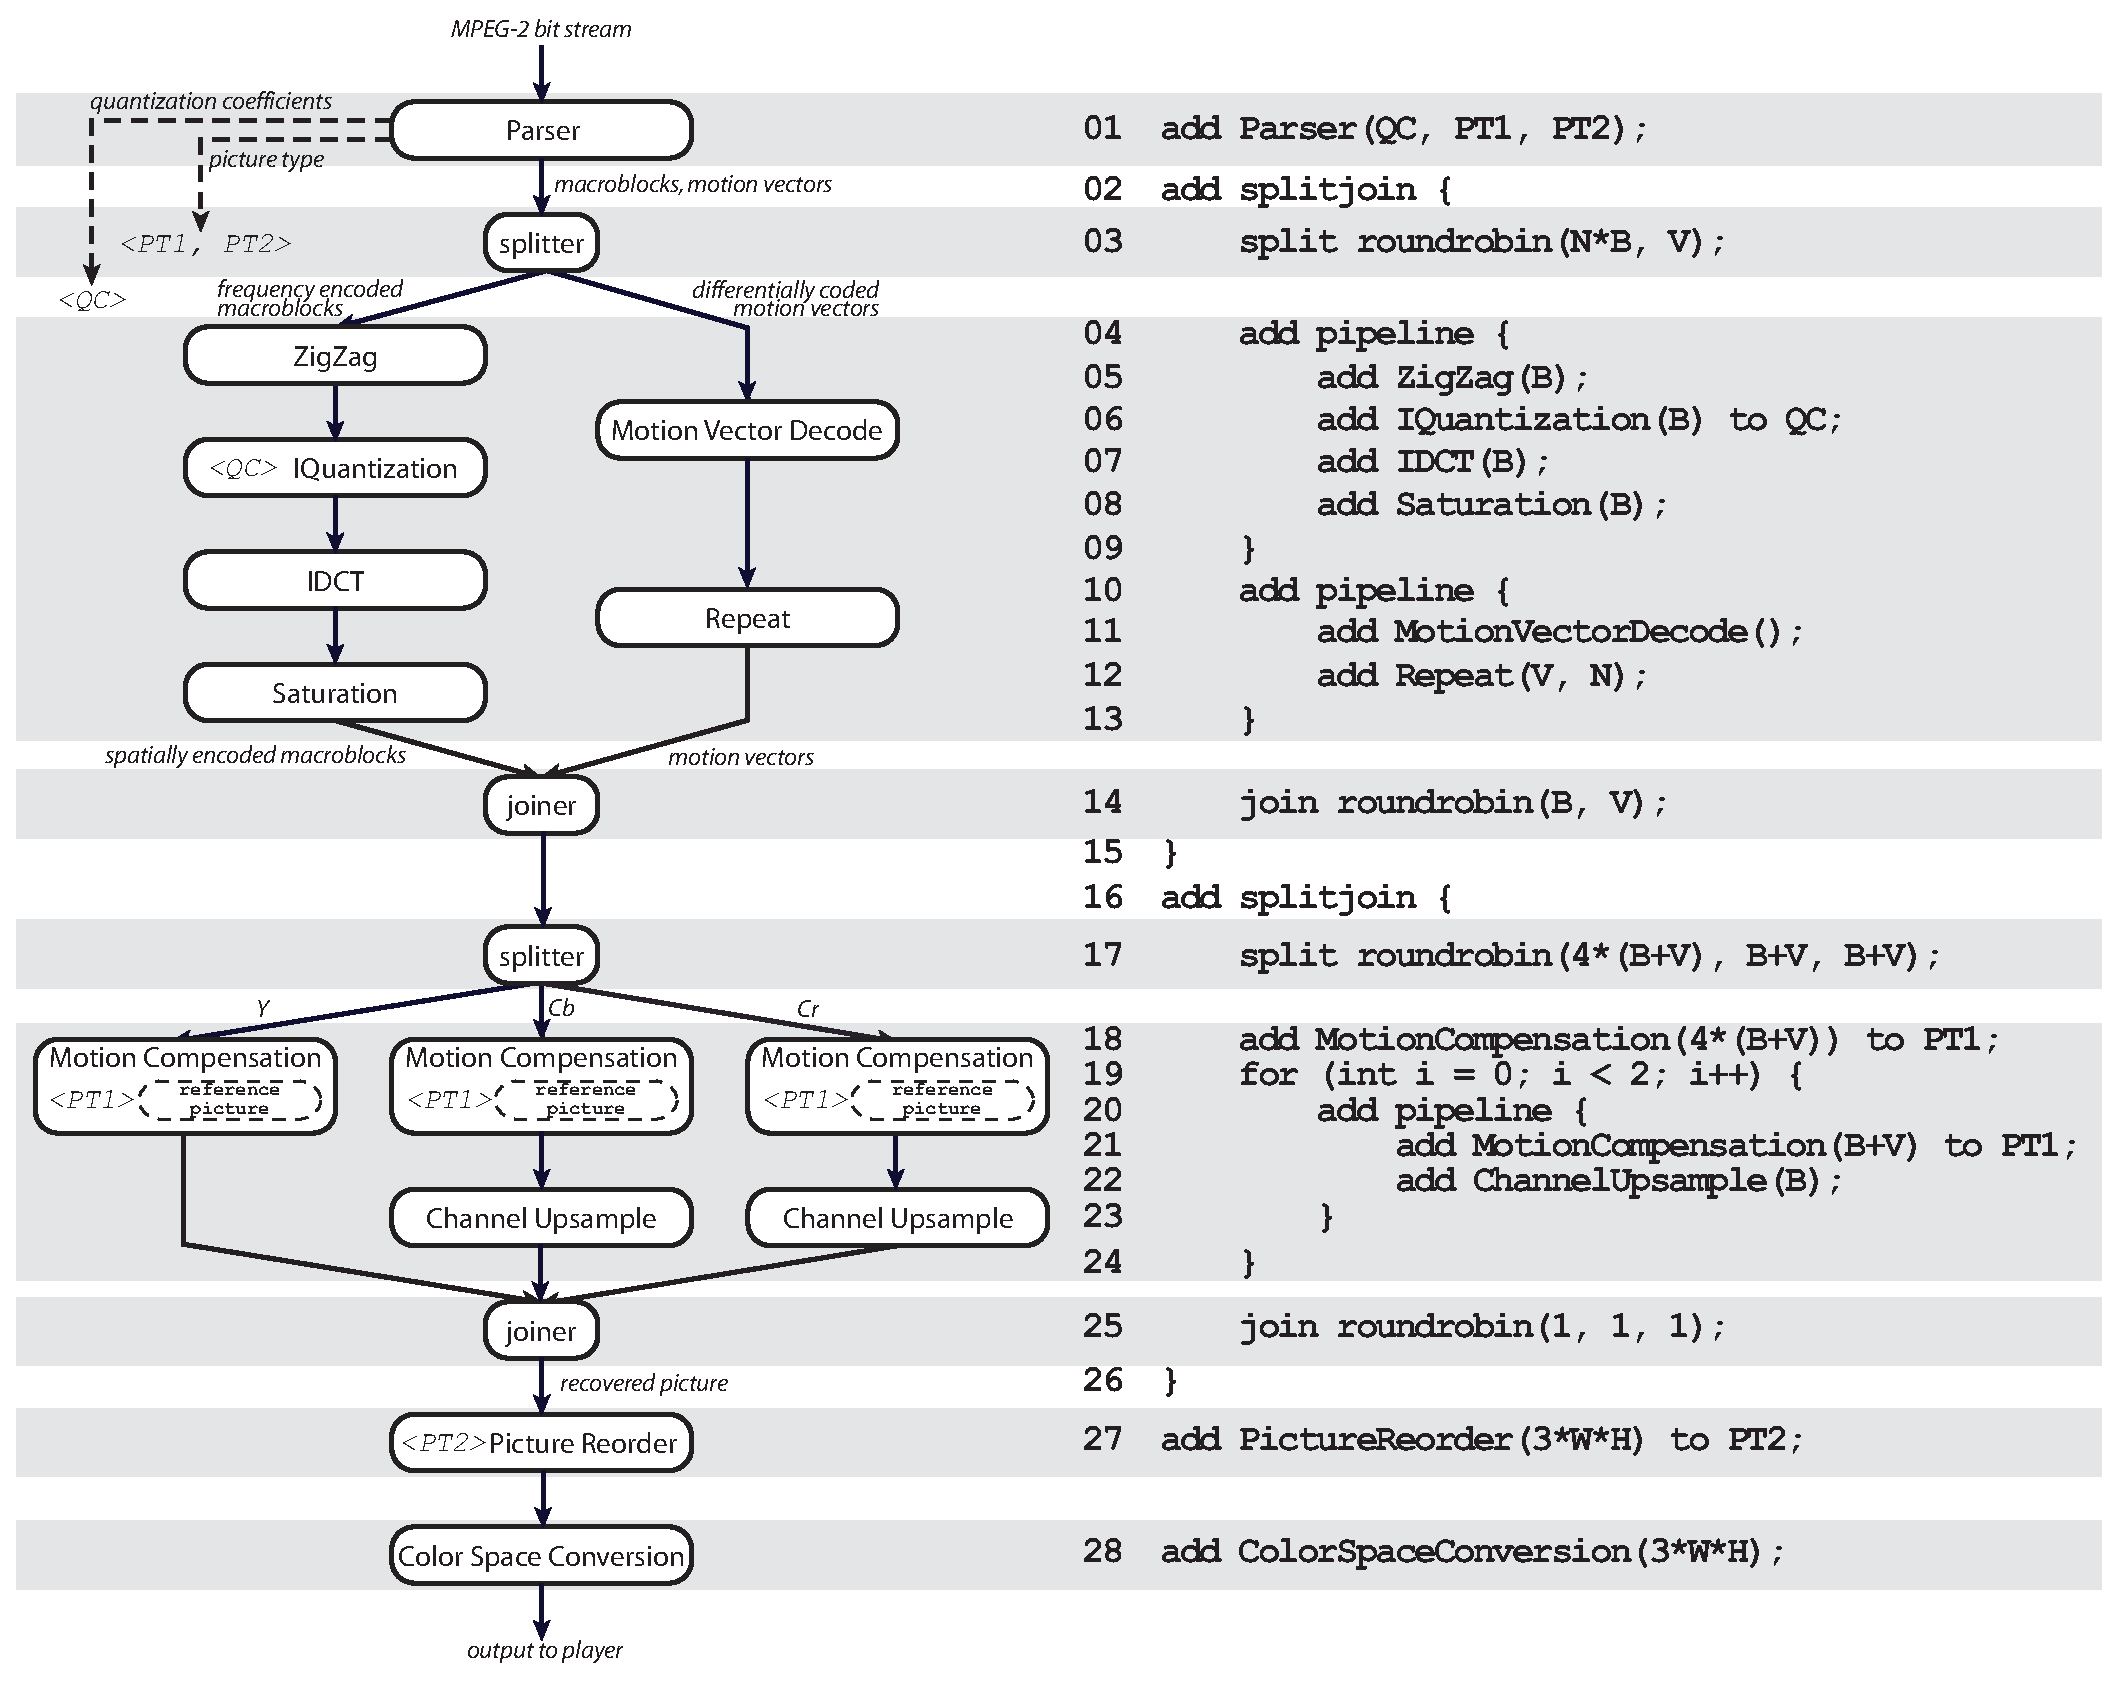
\epsfig{file=decoder_with_code.eps,width=\textwidth}
  \vspace{-22pt}
  \caption{Block diagram of MPEG-2 decoder and corresponding StreamIt code.}
  \vspace{-12pt}
  \label{fig:dec-with-code}
  \end{minipage}
\end{figure}
%%%%

%% \SubSection{Motion Compensation}

% Commented out this section since this information is incorporated into
% the decoder implementation section. - Matt 1/25/06
% An MPEG decoder accepts a bitstream as input and performs Huffman and
% variable run-length decoding (VLD).  This process results in a set of
% quantized, frequency-domain macroblocks and corresponding motion
% vectors.  The decoder inversely quantizes (IQ) the macroblocks and then
% performs an inverse DCT (IDCT) to convert the macroblocks to the
% spatial domain.  For predictively coded macroblocks (e.g., P and B
% pictures), the decoder performs motion compensation (MC) using the
% input motion vectors to find a corresponding macroblock in a
% previously decoded, stored reference picture. This reference
% macroblock is added to the current macroblock to recover the original
% picture data. If the current macroblock is part of an I or P picture,
% then the decoder stores it for future reference.
% Figure~\ref{fig:dec_block} illustrates the decode sequence.

%\begin{figure}[htbp]
%\centerline{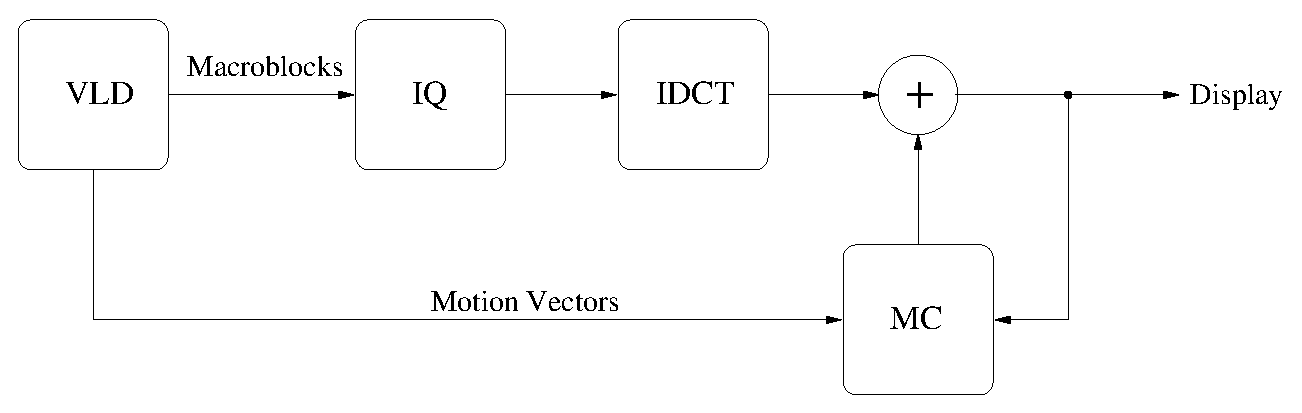
\epsfig{file=dec_block.eps,width=5in}}
%\caption{Block diagram of MPEG-2 decode.}
%\label{fig:dec_block}
%\end{figure}

%% A simple strategy for parallelizing the MPEG-2 decoding can exploit
%% the data parallelism among macroblocks. Using this scheme, the Huffman
%% and run-length decoding is inherently serial, as macroblock boundaries
%% can only be discovered by performing the decode operation.  Once this
%% decode is complete, a parallel implementation can distribute
%% macroblocks to independent streams (using a splitjoin). Each stream
%% performs the inverse quantization, inverse discrete cosine transform,
%% and motion compensation. Furthermore, each stream locally stores
%% reference macroblocks for future motion compensation. Using this
%% strategy, the streams can execute independently with one exception.

%% % TODO: This is the figure showing the macroblock parallelism
%% % I'm not sure where it goes. - Matt
%% \begin{figure*}[t]
%% \vspace{-12pt}
%% %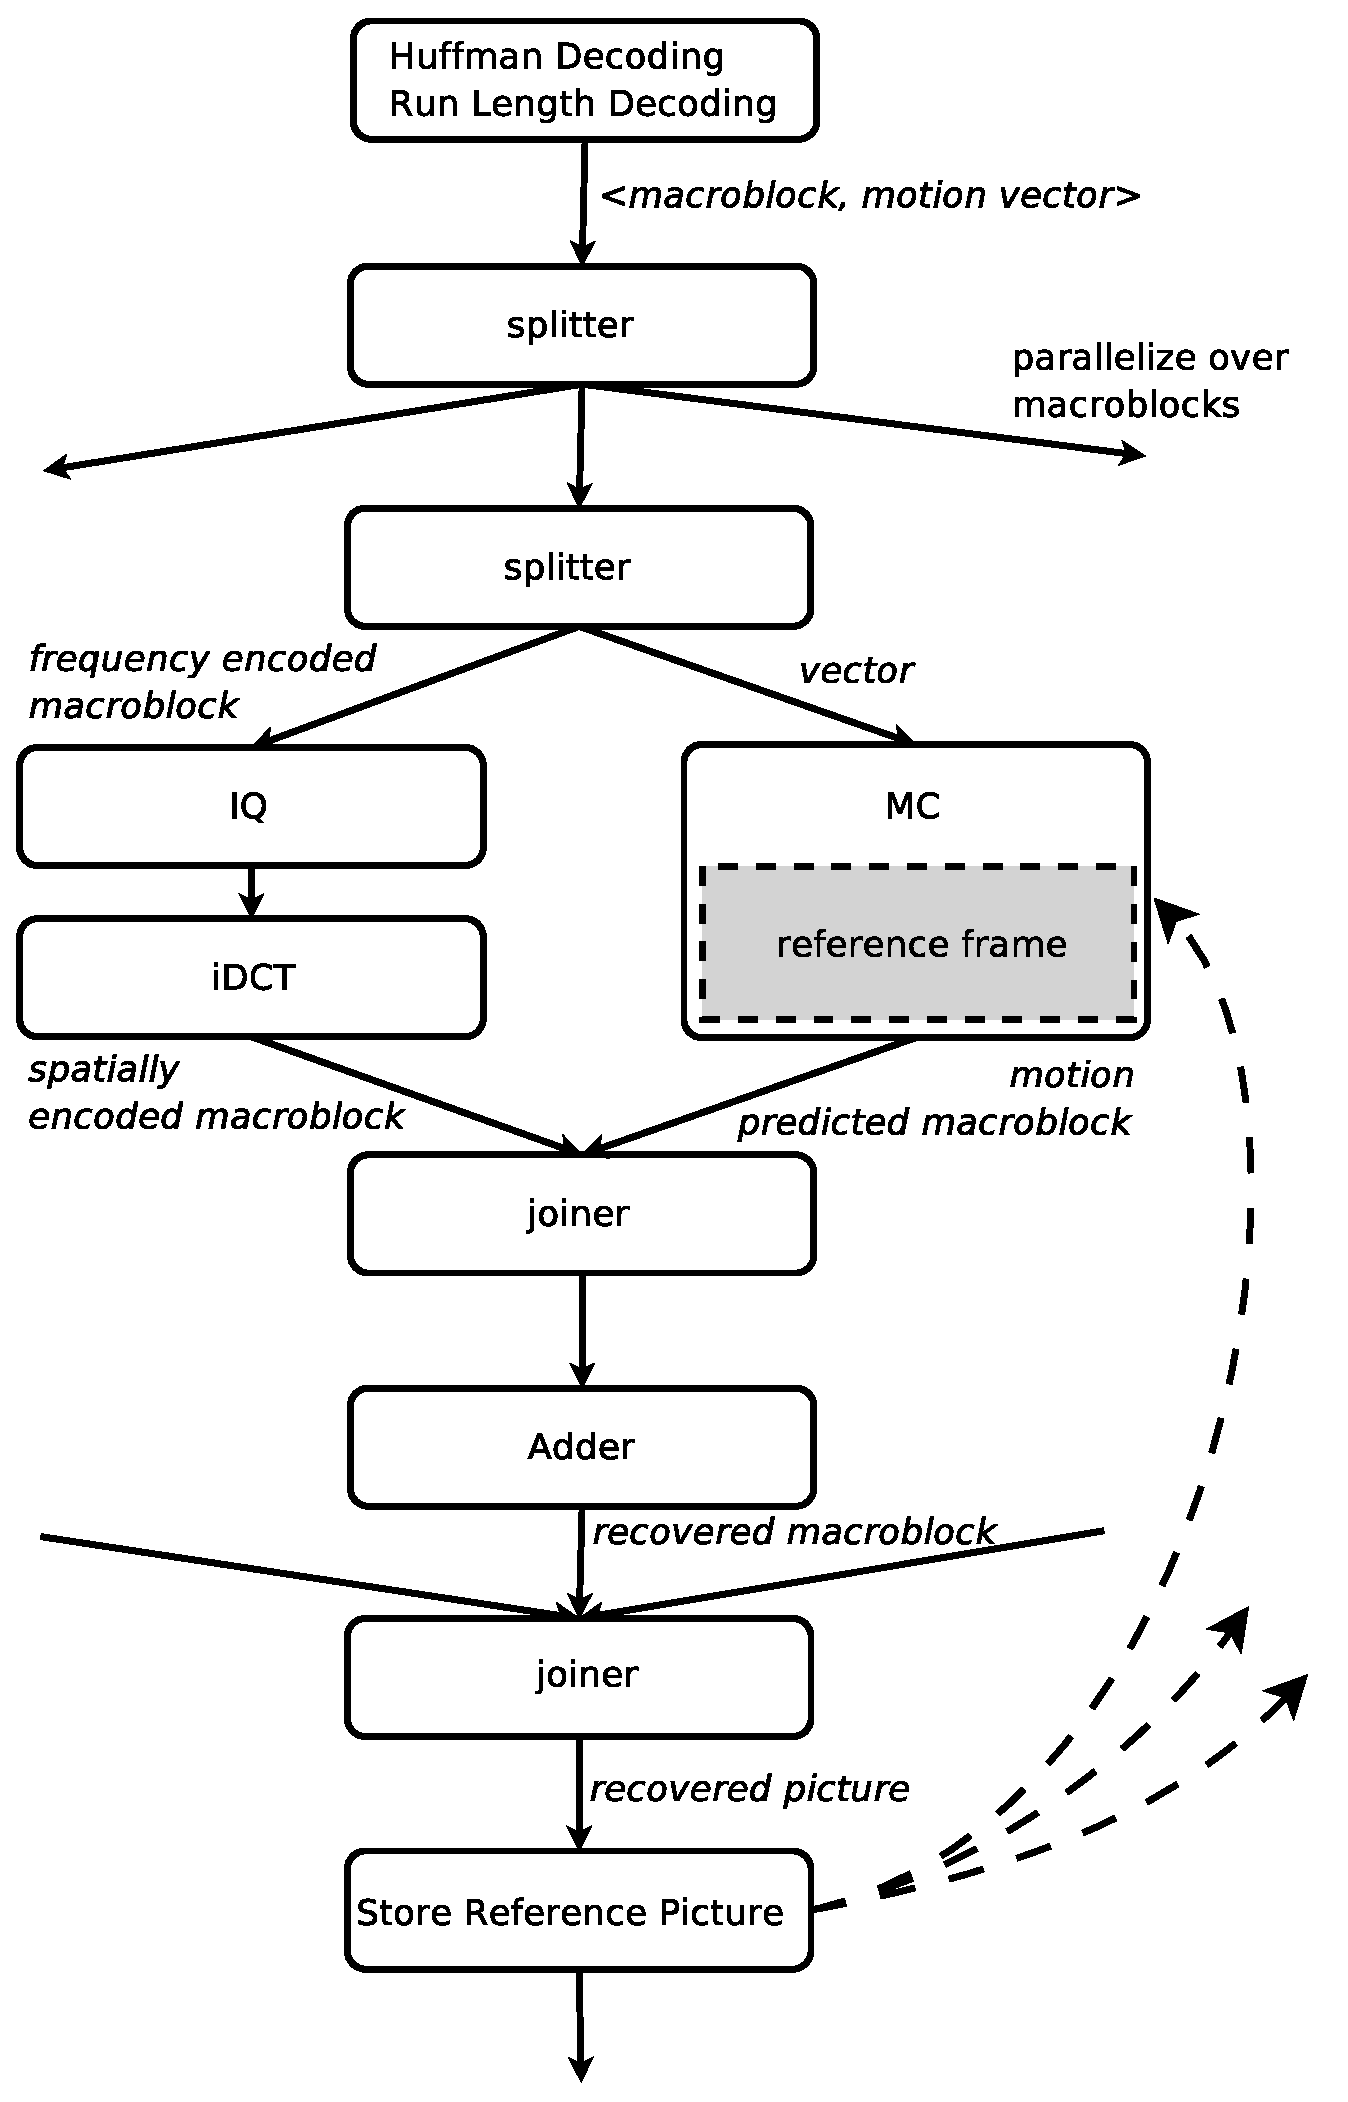
\epsfig{file=decoder_macroblock_parallelism.eps, width=3in}
%% %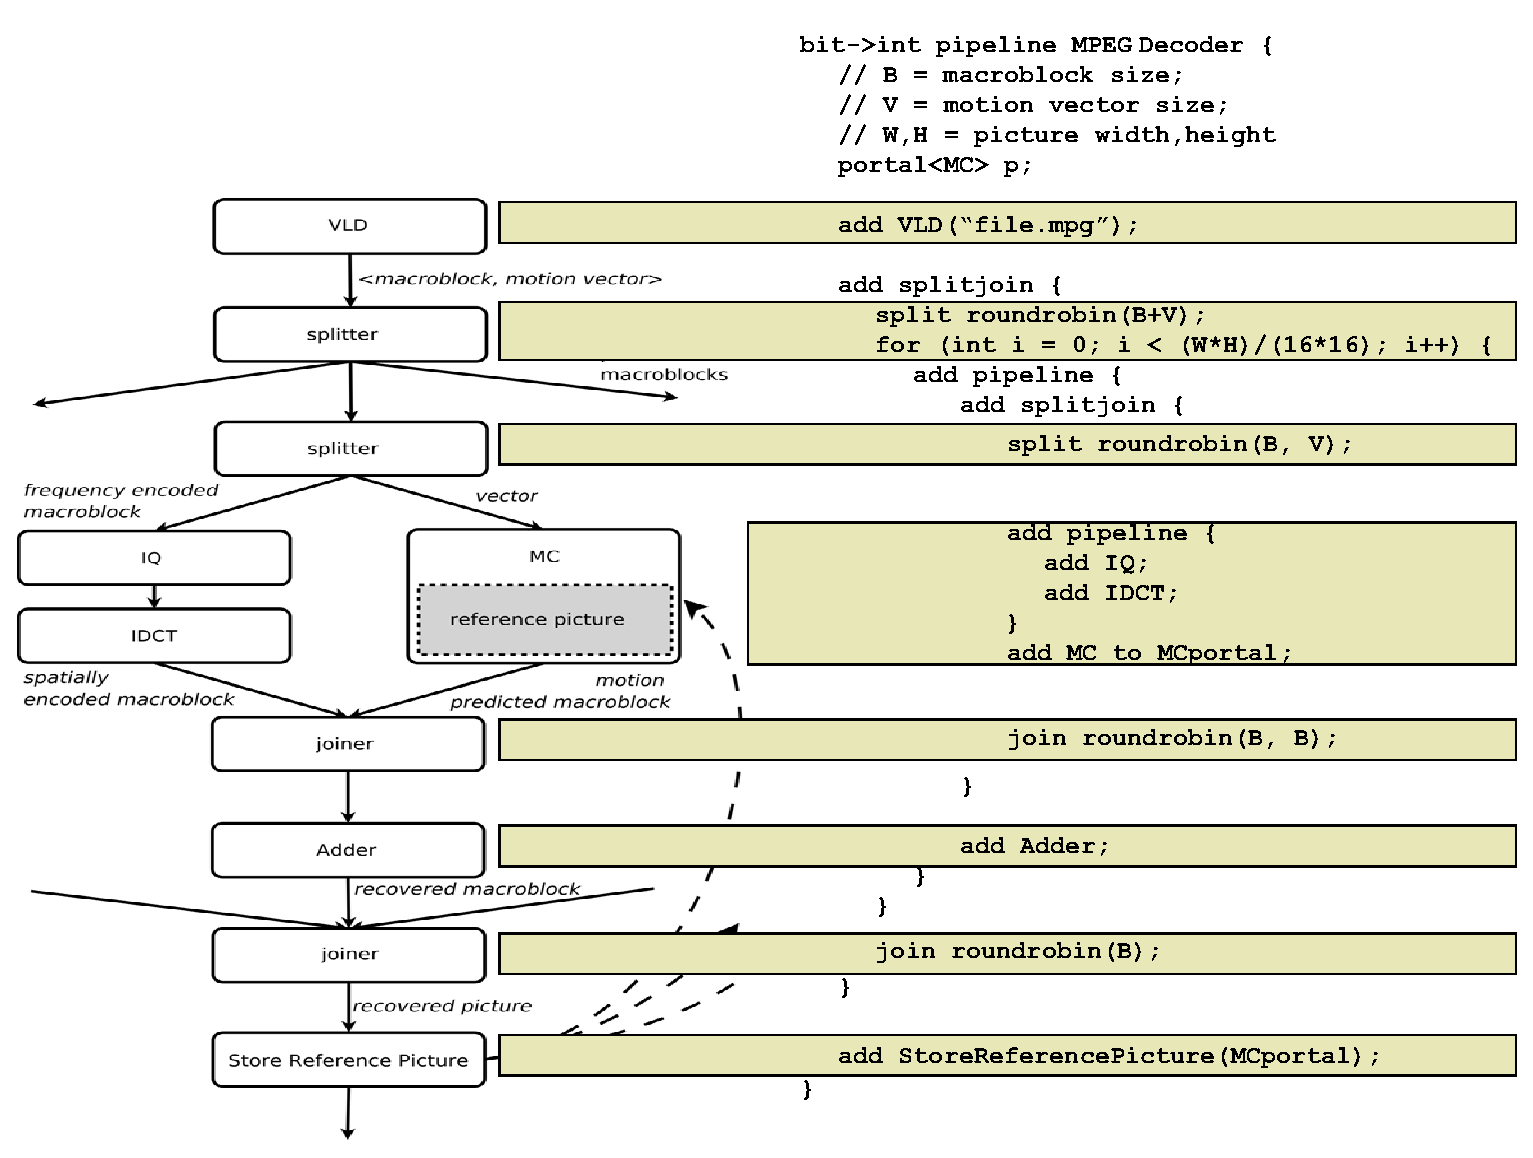
\epsfig{file=decoder-parallel.eps, width=\textwidth}
%% 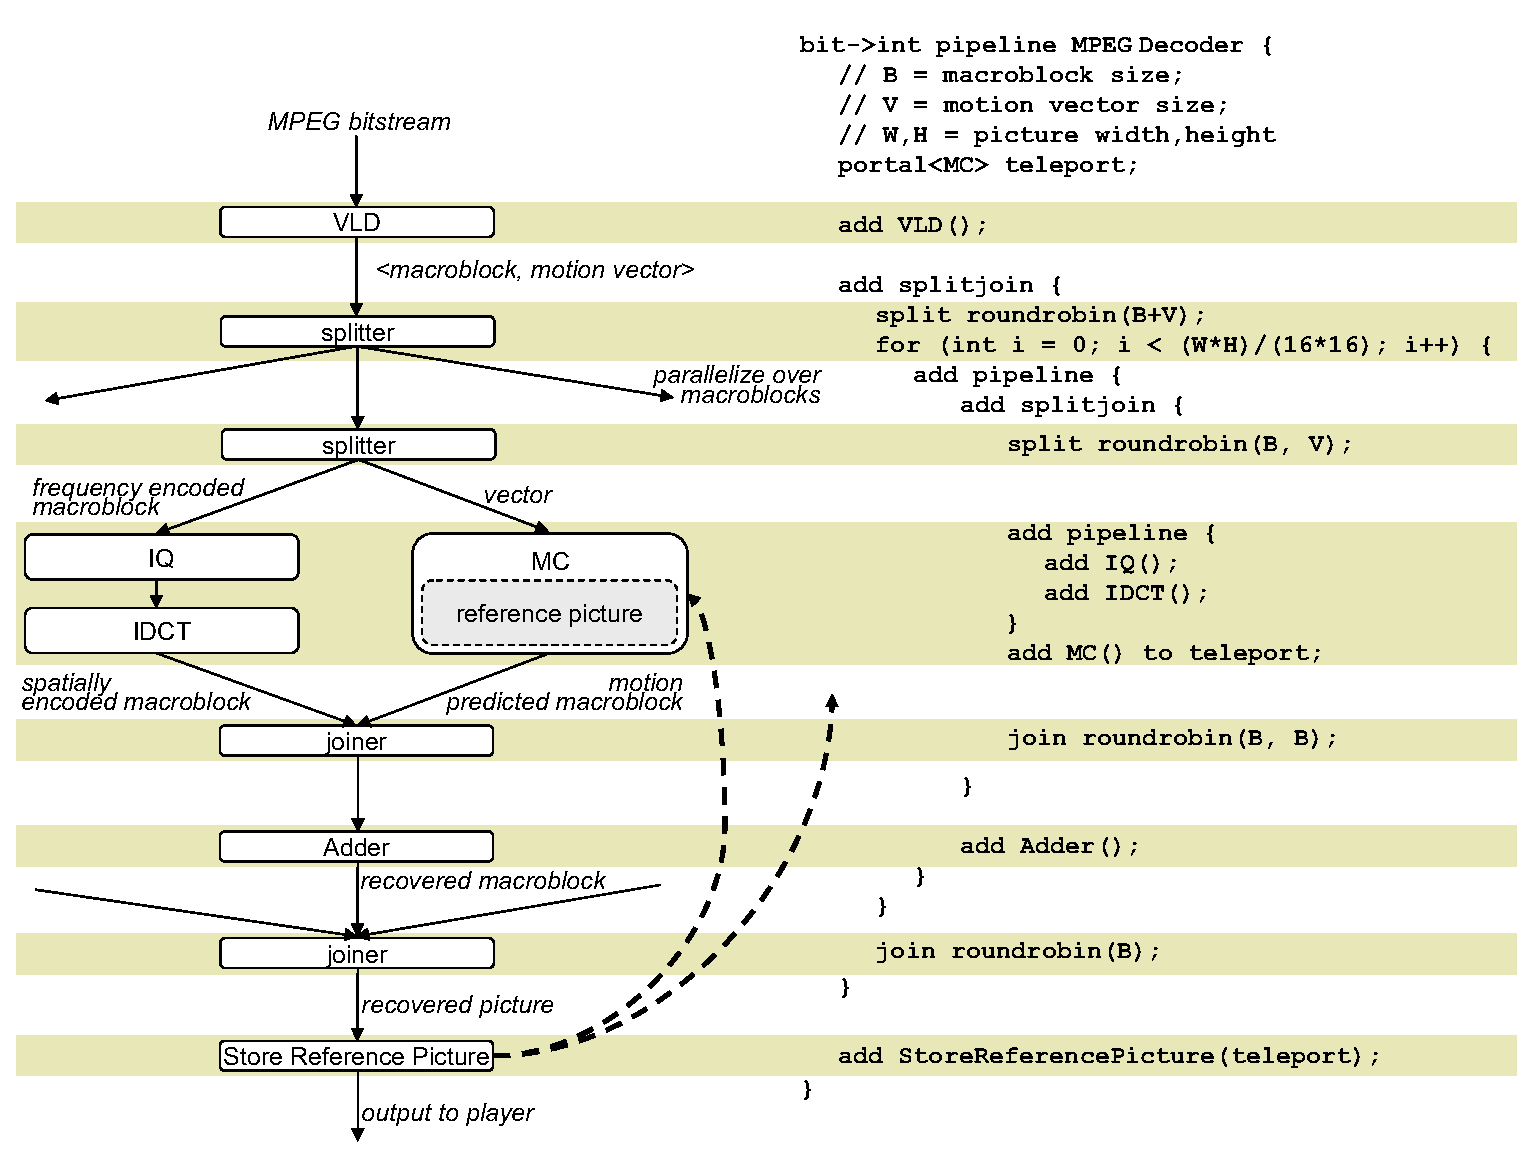
\epsfig{file=decoderpipeline.eps, width=\textwidth}
%% % TODO: Change Matt's 2 am caption.
%% \caption{MPEG-2 decoder exploiting macroblock-level parallelism.}
%% \label{decoder_macroblock_parallelism}
%% \vspace{-6pt}
%% \end{figure*}

%% This exception occurs when a stream is performing motion compensation
%% and the corresponding motion vector indicates a reference macroblock
%% stored in some other stream. In this case, inter-stream communication
%% is required to send the reference data to the requesting stream. This
%% situation is not uncommon, and is more prevalent for higher resolution
%% pictures. A simple scheme for handling this situation is for every
%% stream to broadcast its decoded macroblocks to all other streams. This
%% solution has the benefit of being conceptually easy to understand and
%% implement. StreamIt allows programmers to naturally expose such
%% parallelism.
%% A StreamIt pipeline that operates at macroblock
%% granularity is shown in Figure~\ref{decoder_macroblock_parallelism}. It is
%% worthy to note that there is a high correlation between the stream
%% graph, and the StreamIt syntax describing the pipeline.

%% The implementation can be made more fine grained by exposing the
%% intra-macroblock parallelism. For example, the IQuantization-IDCT
%% pipeline can operate at a block level, rather than at a macroblock
%% granularity. This is easily achieved by encapsulating the  pipeline
%% within a splitjoin to scatter the blocks, operate, and gather the
%% results to recover the parent macroblock.

%% There are many implementation strategies for the decoder, each with
%% varying degrees of exposed parallelism. Of the greatest advantage of
%% the StreamIt implementation is its malleability. The stream graph is
%% easily reconfigured to operate at picture-level granularity (exposing
%% parallelism between chroma channels), macroblock level (exposing even
%% more data-level parallelism), or even at block level (exposing the
%% greatest amount of data-level parallelism).
\chapter{Programmability and Productivity}
\label{chapter:compare}

As previously mentioned, the StreamIt language aims to improve 
programmability for streaming applications. This chapter expands 
on this topic by giving specific instances from the MPEG-2 codec 
implementations where StreamIt improved programmer productivity.

Section~\ref{sec:buffer_management} focusses on StreamIt's 
implicit buffer management. Section~\ref{sec:pipelines_block}
describes how pipelines preserve the block diagram structure
in the program definition and provide a one-to-one mapping with
code. Sections~\ref{sec:expose_data}~and~\ref{section:chroma}
show StreamIt's ability to expose data distribution and
how this leads to a high degree of malleability. 
Section~\ref{sec:hier} describes the advantages of
hierarchical stream graph construction and 
Section~\ref{sec:teleport_useful} the advantages of 
teleport messaging.

Because I particularly want to contrast with 
traditional languages, a number of C code comparisons appear in 
this and the subsequent section. These code examples come from the 
C reference decoder implementation~\cite{reference-mpeg-c} provided 
by the MPEG Software Simulation Group and used in the 
MediaBench~\cite{lee97mediabench} benchmark suite. Because our 
StreamIt code does not support interlacing or certain optional 
bitstream semantics, I have modified the C reference implementation 
to remove that additional functionality, for the purposes of fair 
comparison. The comparison is between the StreamIt decoder of $2282$ 
lines, and the C reference code of $3477$ lines\footnote{As before, line counts 
were generated using \texttt{SLOCcount}~\cite{sloccount}.}. 
I believe this line count comparison is a fair 
quantization of StreamIt's ability to concisely express the MPEG-2 
decoder computations.

\section{Buffer Management}
\label{sec:buffer_management}

\begin{figure}
  \begin{center}
    \begin{minipage}{4in}
      \begin{small}
        \begin{verbatim}
01 static void Add_Block(comp,bx,by)
02      int comp,bx,by;
03 {
04   int cc,i, j, iincr;
05   unsigned char *rfp;
06   short *bp;
08   cc = (comp<4) ? 0 : (comp&1)+1;
09   if (cc==0) {
10     rfp = current_frame[0] + 
11           Coded_Picture_Width*(by+((comp&2)<<2)) + 
12           bx + 
13           ((comp&1)<<3);
14     iincr = Coded_Picture_Width - 8;
15     if (chroma_format!=CHROMA444)
16       bx >>= 1;
17     if (chroma_format==CHROMA420)
18       by >>= 1;
19     rfp = current_frame[cc] + 
20           Chroma_Width*(by+((comp&2)<<2)) + 
21           bx + 
22           (comp&8);
23     iincr = Chroma_Width - 8;
25   }
26   bp = ld->block[comp];
27   for (i=0; i<8; i++) {
28     for (j=0; j<8; j++) {
29       *rfp = *bp++ + *rfp;
30       rfp++;
31     }
32     rfp+= iincr;
33   }
34 }
        \end{verbatim}
      \end{small}
    \end{minipage}
  \end{center}
  \caption{Combining the spatially and temporally decoded data in C.}
  \label{fig:add-filter-in-c}
\end{figure}

\begin{figure}
  \begin{center}
    \begin{minipage}{3in}
      \begin{small}
        \begin{verbatim}
01 int->int filter Add_Block {
02   work pop 2 push 1 {
03     push(pop()+pop());
04   }
05 }
        \end{verbatim}
      \end{small}
    \end{minipage}
  \end{center}
  \caption{Combining the spatially and temporally decoded data in StreamIt.}
  \label{fig:add-filter2}
\end{figure}

Figure~\ref{fig:add-filter-in-c} shows the C code responsible for merging the
spatially and temporally decoded block data\footnote{The original Add\_Block function
performed some unrelated parts of the decoding process as well and was almost 99 lines
long. For comparison purposes the unrelated code is removed.}. Prior to the execution of this
function the IDCT function has generated the motion prediction
error and the motion compensation function has generated the motion prediction. 
These two sets of data are summed to produce the decoded blocks.

Lines 9 through 25 determine the appropriate memory addresses 
for the next block to be processed. Lines 26 to 33 perform the
summation.
Note that line 29 is the only line actually performing the summation. 
The buffer management details dominate every line of code and obscure its functional
purpose. 
The buffer management details are particularly complicated
because the address of the data is dependent on the block's position in a picture,
the size of the video, and the chroma format. The complicated arithmetic
used to adjust buffer indices will make it challenging for a compiler to extract
parallelism. Further complicating any compiler analysis is the function's reuse
 of an input buffer as an output buffer (as reflected in
line 29). 

Reusing buffers is one of many buffer management strategies. The strategy yielding
the best performance depends on the 
target architecture and the size of the buffer. However, the programmer has been
forced to guess about the performance and commit to a particular strategy. 
Also note that a programmer using this function must manually determine 
an execution schedule and buffer sizes that avoid buffer underflow or the premature
overwriting of data.

Now consider the equivalent StreamIt code for adding the decoded block data, shown in
Figure~\ref{fig:add-filter2}. The code itself is almost trivial. The filter 
occurs after a \texttt{roundrobin(1)} joiner merging the prediction error
and the prediction itself. Figure~\ref{fig:motion_prediction_parallel}, 
explained in detail later in Chapter~\ref{chapter:exposing_parallelism}, shows
this filter in the context of the motion compensation stream graph. Note that 
the amount of data this filter processes will 
be dependent on the same chrominance and picture size parameters as the C code
but the buffer management details are hidden from the programmer - they will
be reflected in the data rates of the splitters and joiners surrounding
the filter in the motion compensation graph. At compile
time the compiler makes the decisions about the best buffer management 
strategy~\cite{sermulins05lctes}.  

\section{Pipelines Preserve Block Structure}
\label{sec:pipelines_block}

The pipeline construct preserves the structure implicit in a block diagram.
Figure~\ref{fig:spatial_decoding1} shows a block diagram for spatial decoding
taken from Figures 7-1 and 7-4 of the MPEG-2 specification~\cite{MPEG2}.
Figure~\ref{fig:spatial_decoding0} shows the 
StreamIt code that implements the pipeline. The obvious 
correspondence points to StreamIt's ability to naturally
represent this computation. Note that the quantization
parameters in the diagram are realized as messages in the stream graph.

\begin{figure}[h]
  \center{
    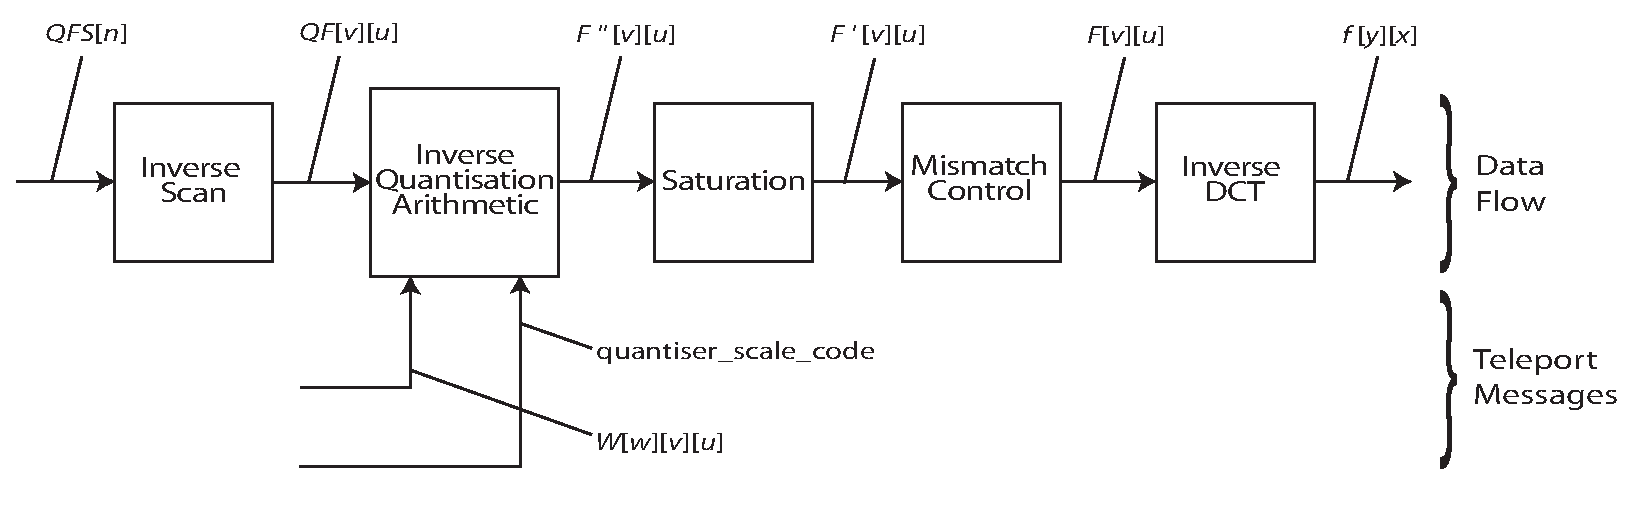
\includegraphics[scale=0.55, angle=0]{./block_decoding.eps}
    \vspace{-12pt}
 	\caption{Block diagram for spatial decoding (from MPEG-2 specification).}
 	\label{fig:spatial_decoding1}
  }
\end{figure}

\begin{figure}
  \begin{center}
    \begin{minipage}{3.5in}
      \begin{small}
        \begin{verbatim}
int->int pipeline BlockDecode(
  portal<InverseQuantization> quantiserData,
  portal<MacroblockType> macroblockType) {

  int[64] Order = {...};
  add ZigZag(64, Order);
  add InverseQuantization() to quantiserData,
                               macroblockType;
  add Saturation(-2048, 2047);
  add MismatchControl();
  add 2D_iDCT(8); // 8x8 2D IDCT
  add Saturation(-256, 255);

}
        \end{verbatim}
      \end{small}
    \end{minipage}
  \end{center}
 	\caption{StreamIt pipeline for spatial decoding.}
 	\label{fig:spatial_decoding0}
\end{figure}

An important detail to note is that each of the filters used in a pipeline
may have different granularities. In this case 
the inverse scan, quantization, and IDCT all operate on blocks of 64 data
values at a time. The mismatch control and saturation blocks are naturally expressed
in terms of a single input and output token. Nowhere must the programmer specify
the number of executions or the execution sequence needed to fully decode a picture
or video. This granularity variance holds through the rest of MPEG-2 as well.
Picture reordering can be expressed in terms of pictures and motion compensation in terms of motion vectors. 
The programmer's burden is eased since he does not have to worry about the rate discrepancies
between filters. 

\section{Natural Exposure of Data Distribution}
\label{sec:expose_data}

\begin{figure}
  \begin{center}
    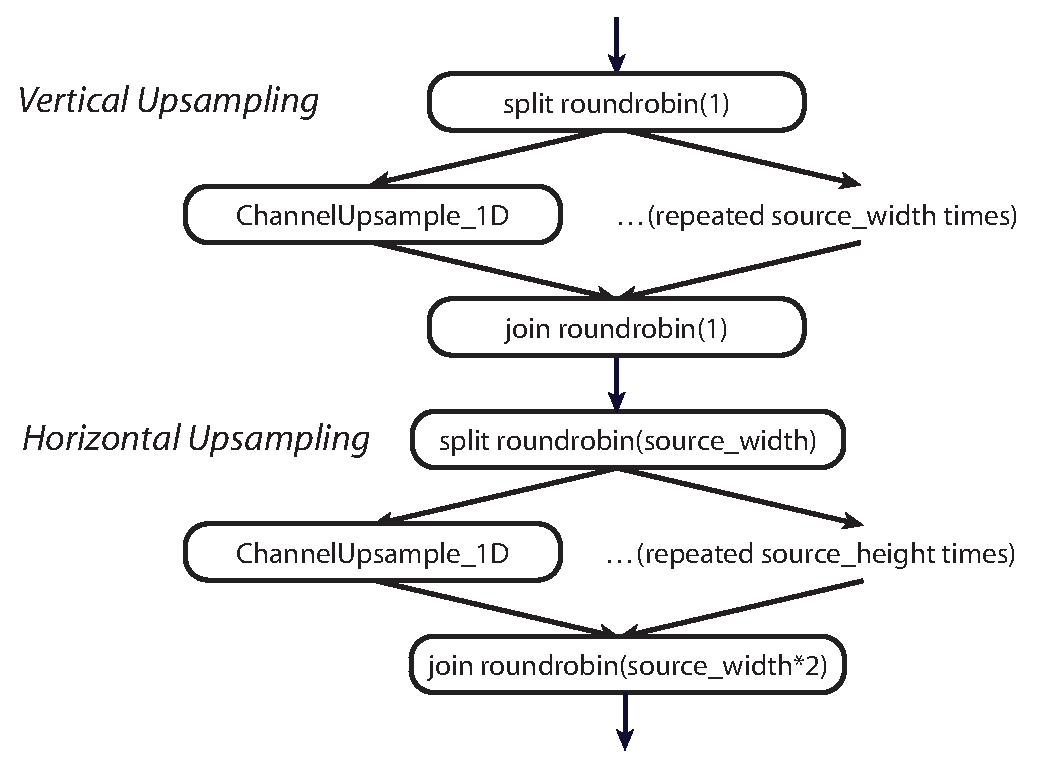
\includegraphics[scale=0.6, angle=0]{./channel_upsampling.eps}
    \caption{2D upsampling decomposed into 1D upsampling}
    \label{fig:how-upsampler-splits-data}
  \end{center}
\end{figure}

\begin{figure}
  \begin{center}
    \begin{minipage}{5.2in}
      \begin{small}
        \begin{verbatim}
int->int splitjoin ChannelUpsample_Vertical(int sourcewidth, 
                                            int sourceheight) {
    split roundrobin(1);
    for (int i = 0; i < sourcewidth; i++) {
        add ChannelUpsample_1D(sourceheight, 0.75, 0.25);
    }
    join roundrobin(1);
}

int->int splitjoin ChannelUpsample_Horizontal(int sourcewidth, 
                                              int sourceheight) {
    split roundrobin(sourcewidth);
    for (int i = 0; i < sourceheight; i++) {
        add ChannelUpsample_1D(sourcewidth, 0.5, 0.5);
    }
    join roundrobin(sourcewidth*2);
}
        \end{verbatim}
      \end{small}
    \end{minipage}
  \end{center}
  \caption{Splitjoins for channel upsampling.}
  \label{fig:upsamplecode}
\end{figure}

The splitjoin construct is a robust mechanism for expressing 
parallelism and data reordering operations. It can be used 
to specify coarse grained parallelism at the highest levels 
of an application because it exposes the independence of computational 
blocks. But it is also useful for describing how a 
computation should be performed, exposing 
coarse grained and fine grained parallelism 
as a byproduct. 

Channel upsampling illustrates this. One can easily 
think of 2D upsampling in terms of 1D upsampling in the vertical 
and horizontal direction\footnote{This is conceptually similar
to the decomposition of a 2D DCT, discussed 
later in Section~\ref{sec:2d_dct}. 
In this case the channel upsampling represents a smaller
amount of work and the splitjoin is more interesting for its
ability to efficiently express the transformation than its ability
to expose parallelism.}. The 
natural way to express upsampling a picture in either 
direction is as a parallel computation on every row or 
column of the picture. The building block is a one-dimensional 
upsampling filter that takes in a pair of weights used for 
interpolation between points. The weights are different for 
horizontal and vertical upsampling because MPEG-2 downsamples 
horizontally by removing pixels, and vertically by displacing 
them. 
The vertical upsampler splits the 
data by column and the horizontal upsampler splits the data 
by row. Figure~\ref{fig:how-upsampler-splits-data} illustrates 
the procedure and Figure~\ref{fig:upsamplecode} shows the 
StreamIt code that implements the process. The C reference
implementation implements upsampling as a series of loops
wrapped around a one dimensional upsampling kernel. In this
case the code looks similar to the StreamIt code. However,
the StreamIt \texttt{for} loops represent graph topology
resolved at initialization time. The C compiler must analyze
the body of the loops to extract parallelism.

\section{Code Malleability}
\label{section:chroma}

\begin{figure}
\begin{center}
  \begin{minipage}[t]{4.8in}
    \begin{small}
      \begin{verbatim}
   /* Y */
01 form_component_prediction(src[0]+(sfield?lx2>>1:0),
02                           dst[0]+(dfield?lx2>>1:0),
03                           lx,lx2,w,h,x,y,dx,dy,average_flag);
04 if (chroma_format!=CHROMA444)  {
05    lx>>=1; lx2>>=1; w>>=1; x>>=1; dx/=2;
06 }
07 if (chroma_format==CHROMA420)  {
08   h>>=1; y>>=1; dy/=2;
09 }
   /* Cb */
10 form_component_prediction(src[1]+(sfield?lx2>>1:0),
11                           dst[1]+(dfield?lx2>>1:0),
12                           lx,lx2,w,h,x,y,dx,dy,average_flag);
   /* Cr */
13 form_component_prediction(src[2]+(sfield?lx2>>1:0),
14                           dst[2]+(dfield?lx2>>1:0),
15                           lx,lx2,w,h,x,y,dx,dy,average_flag);    
      \end{verbatim}
    \end{small}
  \end{minipage}
  \caption{C code excerpt for handling
           4:2:0 and 4:2:2 chroma formats.}
  \label{fig:chroma-format-code-C}
\end{center}
\end{figure}

\begin{figure}
\begin{center}
  \begin{minipage}[t]{3.5in}
    \begin{small}
      \begin{verbatim}
// B = amount of data per block
// V = amount of data per motion vector
add splitjoin {
  split roundrobin(4*(B+V), B+V, B+V);
  add MotionCompensation(4*(B+V)) to PT1;
  for (int i = 0; i < 2; i++) {
    add pipeline {
      add MotionCompensation(B+V) to PT1;
      add ChannelUpsample(B);
    }
  }
  join roundrobin(1, 1, 1);
}
      \end{verbatim}
    \end{small}
  \end{minipage}
  \caption{Original StreamIt code excerpt for handling
           4:2:0 chroma format only.}
  \label{fig:chroma-format-code-streamit-previous}
\end{center}
\end{figure}

\begin{figure}
\begin{center}
  \begin{minipage}[t]{3.5in}
    \begin{small}
      \begin{verbatim}
// C = blocks per chroma channel 
//     per macroblock 
// C = 1 for 4:2:0, C = 2 for 4:2:2
// B = amount of data per block
// V = amount of data per motion vector
add splitjoin {
  split roundrobin(4*(B+V), 2*C*(B+V));
  add MotionCompensation(4*(B+V)) to PT1;
  add splitjoin {
    split roundrobin(B+V, B+V);
    for (int i = 0; i < 2; i++) {
      add pipeline {
        add MotionCompensation(B+V) to PT1;
        add ChannelUpsample(C*B);
      }
    }
    join roundrobin(1, 1);
  }
  join roundrobin(1, 1, 1);
}
      \end{verbatim}
    \end{small}
  \end{minipage}

  \caption{StreamIt code excerpt for handling
           4:2:0 and 4:2:2 chroma formats.}
  \label{fig:chroma-format-code-streamit}
\end{center}
\end{figure}

\begin{figure}
  \begin{center}
    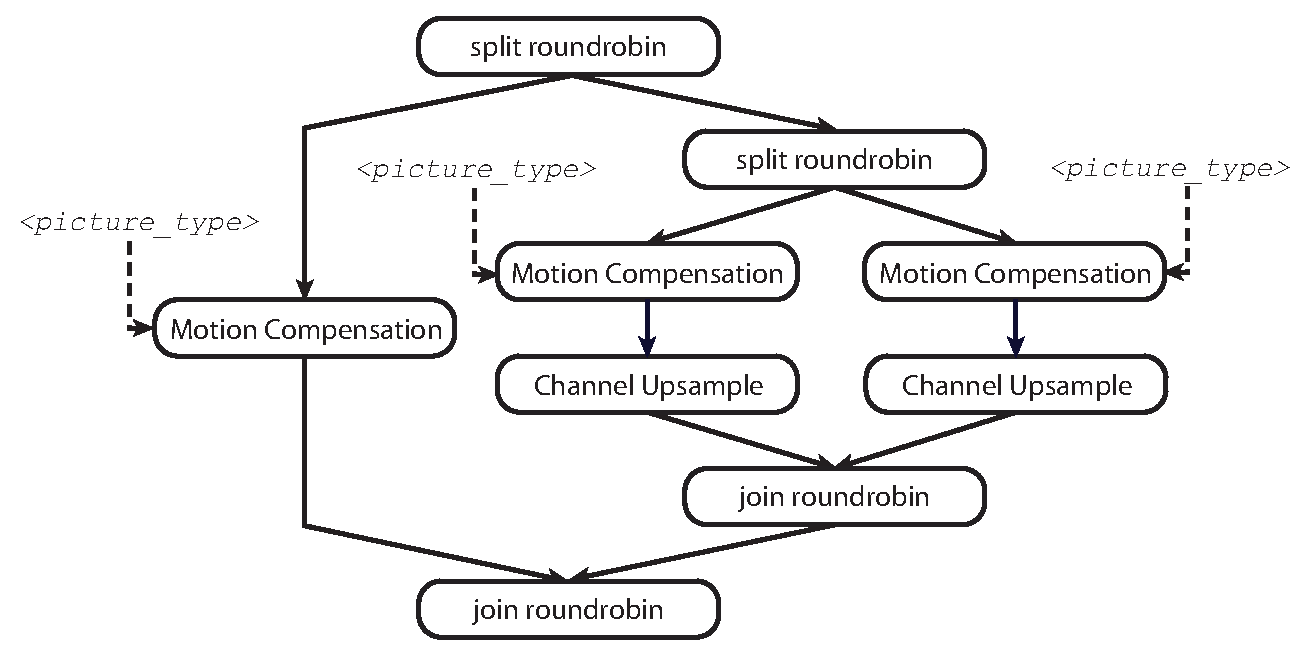
\includegraphics[scale=0.5, angle=0]{./chroma_splitjoin.eps}
    \caption{Modified subgraph for handling 4:2:0 and 4:2:2 chroma formats.}
    \label{fig:chroma-format-graph}
  \end{center}
\end{figure}

A noteworthy aspect of the StreamIt implementation is its
malleability. I illustrate this by outlining how the decoder
implementation is modified to support both 4:2:0 and 4:2:2 chroma
formats (see Section~\ref{section:picture_decomp}). 
The conceptual difference between chroma formats is merely a change in
downsampling ratio. The implementation difference is that the 4:2:0 format
represents a macroblock with six blocks, and the 4:2:2 with 8 blocks. This
change affects the data rates, and the data splitting ratios between color channels. 
In the C reference code, the change requires adjustments to buffer sizes, array lengths, array
indices, loop bounds, and various pointer offsets. The reference implementation
uses a \textbf{chroma flag} to dictate control flow and alternate
index/offset calculations in 43 locations in the code. As an example,
Figure~\ref{fig:chroma-format-code-C} shows a code fragment from the
\texttt{form\_prediction} routine in
\texttt{recon.c}. The function calls a
subroutine to perform the motion compensation on each of the three
color channels, passing in array offsets to a global array holding the
data. Lines 4-6 adjust values used for address calculations to handle
the 4:2:2 and 4:2:0 chroma formats, and lines 7-9 provide additional
adjustments for the 4:2:0 format. While these offset adjustments are
necessary in C, they are difficult for programmers and make the code
hard to understand.

In StreamIt, I modified 31 lines and added 20 new lines to support
the 4:2:2 format. Of the 31 modified lines, 23 were trivial changes to
introduce the chroma format as a stream parameter. The greatest
substantial change was to the color channel splitter, previously
illustrated on line 17 of Figure~\ref{fig:dec-with-code}. In the case
of a 4:2:2 sampling rate, the chrominance data, as it appears on the
input tape, alternates between each of the two chrominance
channels, as previously shown in Figure~\ref{fig:chroma_format}.
Thus, a nested splitjoin is used to properly recover the
chrominance channels. 

The code for the old splitjoin before the chroma format
support modifications is shown in 
Figure~\ref{fig:chroma-format-code-streamit-previous}.
The code for the new splitjoin is shown in 
Figure~\ref{fig:chroma-format-code-streamit} and
illustrated in Figure~\ref{fig:chroma-format-graph}.  
In the StreamIt code, the chroma
format explicitly dictates control flow in only 9 locations. Of
course, chroma format changes have effects on scheduling 
and buffer management, but this is transparent to the programmer.

\section{Hierarchical Construction vs Functional Calls}
\label{sec:hier}

Preserving the block structure in the program definition is important for
programmer productivity and maintaining code malleability. 
Figure~\ref{fig:call-diagram}
shows what happens to the block diagram in a traditional language. This figure
represents a simplified call trace for the MPEG-2 decoder in C. 
Note that each component must be wrapped in loops determining the exact number 
of iterations the component must run to fully decode a picture or video. 
Data is stored in global buffers and addresses to these buffers are passed between
functions, so the code structure fails to reflect the actual movement of data.
Finally, notice that the functions for parsing, motion compensation, and spatial decoding are
intermixed in the code for performance reasons.
The StreamIt compiler can interleave the phases of execution to provide performance
but this does not require the programmer to mix functional code.

\begin{figure}[h]
  \begin{center}
    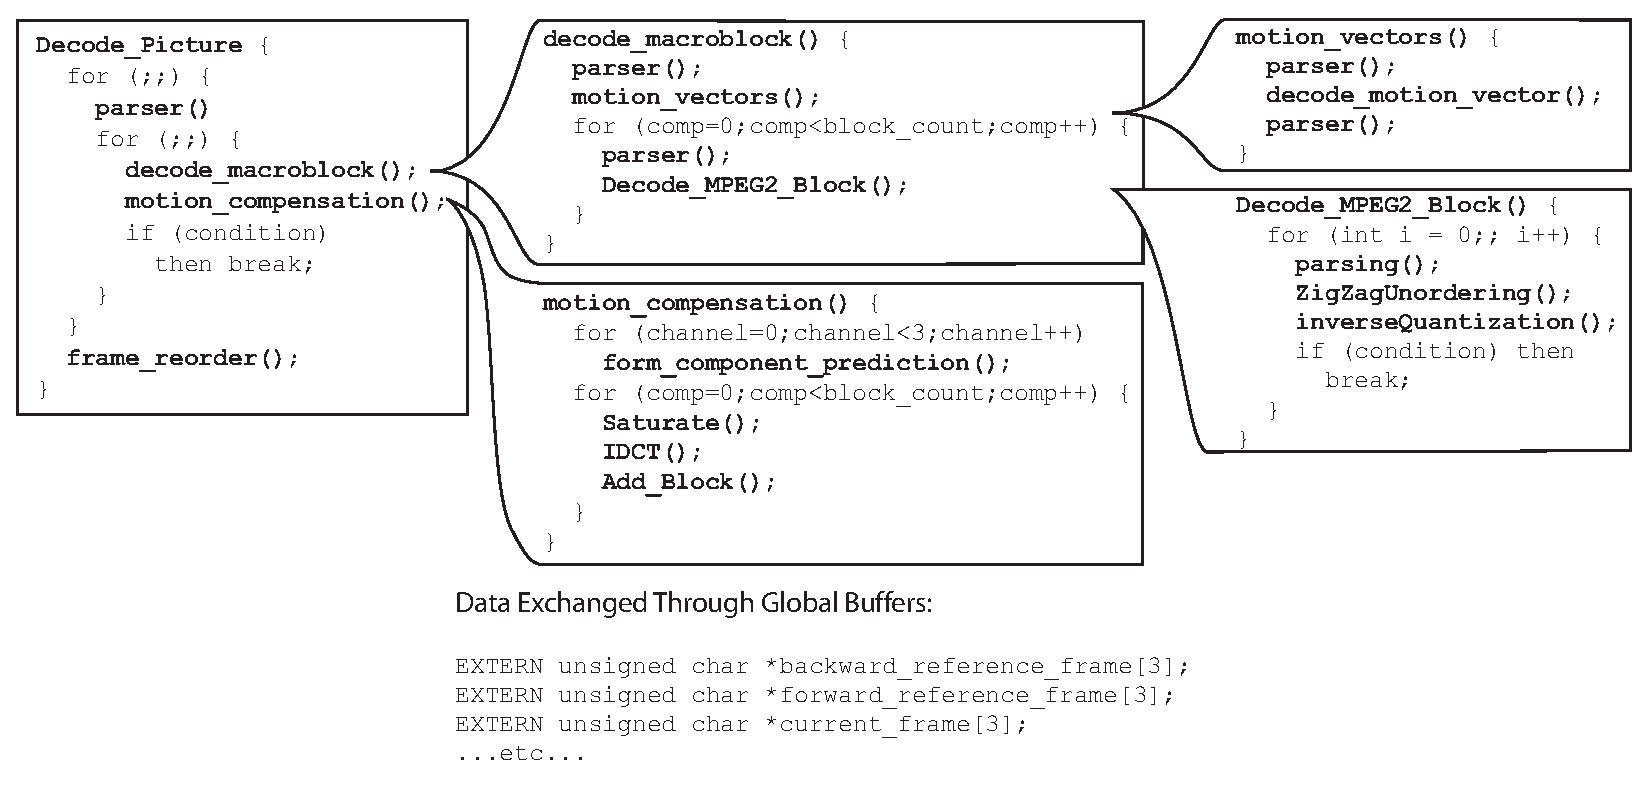
\includegraphics[scale=0.5, angle=0]{./call_diagram.eps}
    \caption{Simplified call-trace diagram for C decoder.}
    \label{fig:call-diagram}
  \end{center}
\end{figure}

\section{Usefulness of Teleport Messaging}
\label{sec:teleport_useful}

Teleport messaging is a useful language construct, as 
demonstrated by its importance in handling control messages 
in the decoder and encoder. 
Figures~\ref{table:enumerate_messages_decoder}~and~\ref{table:enumerate_messages_encoder} 
show the important control parameters that are sent by 
teleport messages in the MPEG-2 codecs. The number of 
subscribers for each message type highlights the usefulness 
of messages. 

\begin{figure}[h]
  \begin{center}
\begin{minipage}{\textwidth}
\renewcommand{\thempfootnote}{
  \arabic{footnote}
}
    \begin{tabular}{|p{1.7in}|l|l|p{0.9in}|p{0.9in}|}
\hline
\textbf{Message Content} & \textbf{Frequency} & \textbf{Regular} & \parbox{0.9in}{\textbf{Number of\\ Subscribers}} & \parbox{0.91in}{\vspace{0.04in} \textbf{Number of\\Subscriber\\Types} \vspace{0.04in}} \\
\hline
quantization scale code & macroblock & no & 2 & 2 \\
quantization tables & video & yes & 2 & 2 \\
macroblock type & macroblock & yes & 4 & 2 \\
picture type & picture & yes & 4 & 2 \\
motion vector resets & macroblock & no & 1 & 1 \\
\addtocounter{footnote}{1}
reference pictures & picture & no & many\footnote{One for every block in all color channels over a picture.} & 1 \\
\hline
    \end{tabular}
\end{minipage}
  \end{center}
  \caption{Important control parameters sent through the decoder using teleport messaging.}
  \label{table:enumerate_messages_decoder}
\end{figure}

\begin{figure}[h]
  \begin{center}
\begin{minipage}{\textwidth}
  \renewcommand{\thempfootnote}{
\arabic{footnote}
}
     \begin{tabular}{|p{1.7in}|l|l|p{0.9in}|p{0.9in}|}
\hline
\textbf{Message Content} & \textbf{Frequency} & \textbf{Regular} & \parbox{0.9in}{\textbf{Number of\\ Subscribers}} & \parbox{0.91in}{\vspace{0.04in} \textbf{Number of\\ Subscriber\\ Types} \vspace{0.04in}} \\
\hline
quantization scale code & macroblock & no & 2 & 2 \\
quantization tables & video & yes & 1 & 1 \\
macroblock type & macroblock & yes & 4 & 2 \\
picture type & picture & yes & 4 & 4 \\
\addtocounter{footnote}{1}
reference pictures & picture & no & many\footnote{Once for every macroblock in all color channels over a picture.} & 2 \\
\hline
    \end{tabular}
\end{minipage}
  \end{center}
  \caption{Important control parameters sent through the encoder using teleport messaging.}
  \label{table:enumerate_messages_encoder}
\end{figure}

Messaging's impact on programmability is evident by 
considering how the C code exposes control relevant information. 
The C code passes data and control parameters through function 
parameters and a global address space. Figure~\ref{fig:c-arrow-diagram} shows the functional
units in the C decoder\footnote{A functional unit might contain multiple functions with
similar or related behaviors.}, the input bitstream, output video, and the shared 
address space. Arrows represent communication dependencies between the blocks. 
While the C implementation is natural --- for C code --- it would be difficult for a 
programmer or compiler to extract 
parallelism\footnote{Because
the analysis of data access patterns is complicated and 
correctness verification for optimizations becomes impractical, 
a compiler will make a pessimistic decision.}.

\begin{figure}[h]
  \begin{center}
    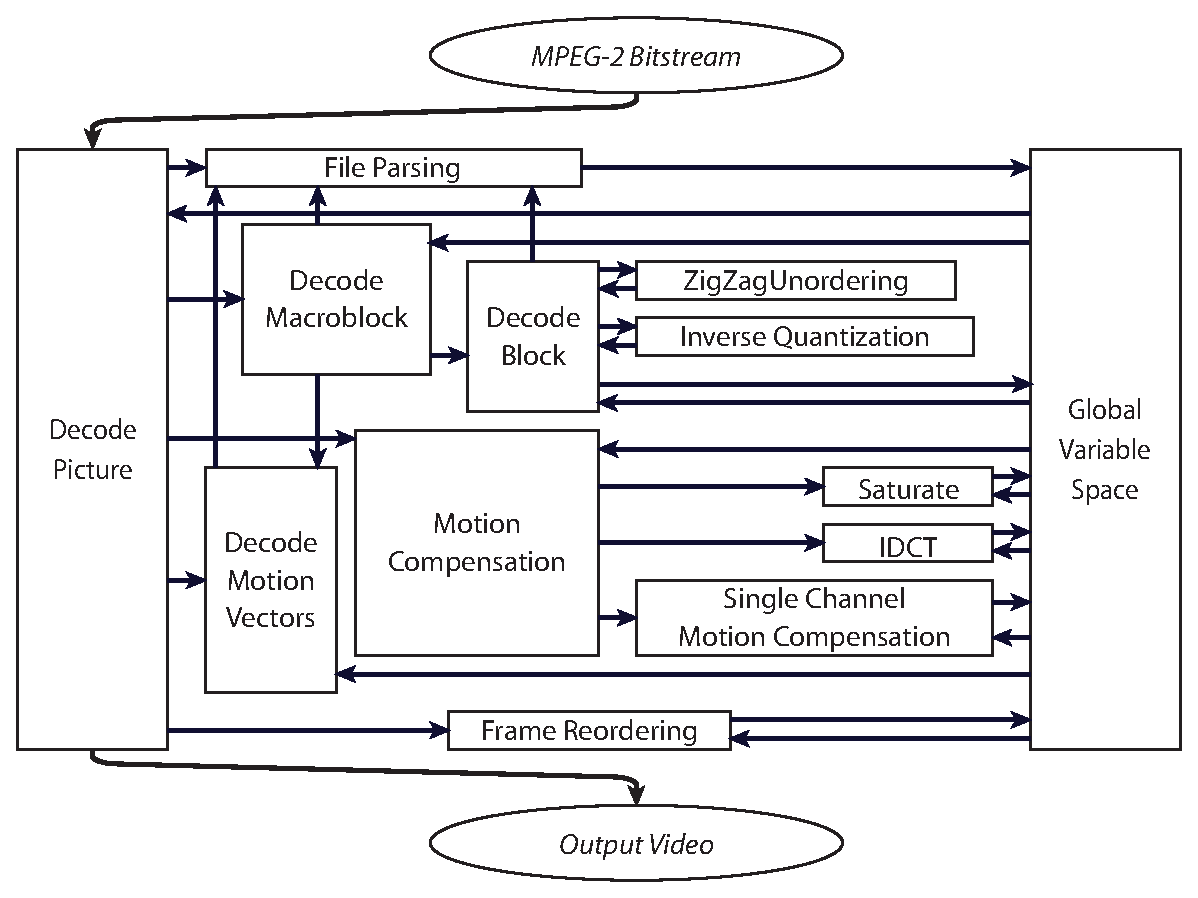
\includegraphics[scale=0.7, angle=0]{./functional_units.eps}
    \caption{Communication dependencies between functional units in the C code.}
    \label{fig:c-arrow-diagram}
  \end{center}
\end{figure}

Teleport messaging provides a point to point connection layer 
which a programmer can emulate in the dataflow layer by 
embedding control parameters in the data channels. While
StreamIt provides the feedback loop construct
to send information upstream, messaging is often more
appropriate for altering upstream state. 

Upstream reference frame passing in the encoder is used as an example. 
A feedback loop structure is impossible here, due to the fact that 
only some pictures should be sent upstream as reference pictures, 
and the information about which pictures to send upstream is not 
available at compile time. This would require the feedback loop to 
process messages regarding picture type and implement a dynamic 
rate splitter and joiner. This is not intuitive to implement, 
nor would it be easy for the compiler to analyze. Without B 
pictures the feedback loop structure needed to ensure that 
each motion estimation filter received the right reference frame 
immediately before the first block of a picture would still be 
non-trivial. Replacing the messaging scheme with a feedback loop 
would also effectively require the motion estimation filters to 
operate at a picture granularity, since each work execution 
would receive a reference picture, and this would limit 
parallelism by preventing estimation to be expressed at a block 
granularity. 

This chapter has given specific instances of where StreamIt improved
programmer productivity. Personal qualitative observations on the entire
implementation process are also pertinent. I found programming in StreamIt
to be very intuitive.
MPEG-2 decomposed naturally into concise independent filters. 
Filters make a program more modular than equivalent C code, 
which made it easy to change the encoder and decoder
stream graphs as my understanding of MPEG-2 improved. For the purposes
of correctness verification and performance comparisons it was much easier
to extract functional units from the StreamIt code than the C code.


\chapter{Expressing Parallelism}
\label{chapter:exposing_parallelism}

Multimedia codecs such as MPEG-2 demand high performance because of throughput
requirements. An online encoder or decoder must be capable of realtime performance,
which can be as high as 60 fps. An offline encoder is less constrained but minimizing
total runtime is still a concern. Since traditional CPU clock scaling has ended,
meeting throughput demands requires parallel scalable implementations. 
Critical to these implementations is the compiler's ability to detect parallelism
in a program specification. 
This section examines how parallelism was successfully 
realized in the MPEG-2 codecs and how the StreamIt language made this task easy. The 
parallelism discussed in this section is exposed through the stream graph 
topology rather than by changing any underlying algorithms. This section ignores 
parallelizing MPEG-2 codecs across GOPs; since GOPs are coded independently, 
this is embarrassingly parallel and trivial. I also include proof of 
concept results showing that the StreamIt implementation scales on multicore
architectures.

\section{Splitjoins Express Data Parallelism}

One particularly noteworthy aspect of splitjoins is the ability to define 
their internal topology using the for-loop construct. The for-loop, unrolled at 
instantiation time, makes the degree of parallelism and the stream topology
itself parameterizable. 
This feature makes it easy for the programmer to concisely express a data parallel 
computation. The code responsible for channel upsampling, shown in 
Figure~\ref{fig:upsamplecode}, expresses a massively data parallel computation in 
this way. 

\section{Hierarchical Streams Expose High Degrees of Parallelism}
\label{sec:2d_dct}

\begin{figure}[h]
  \begin{center}
    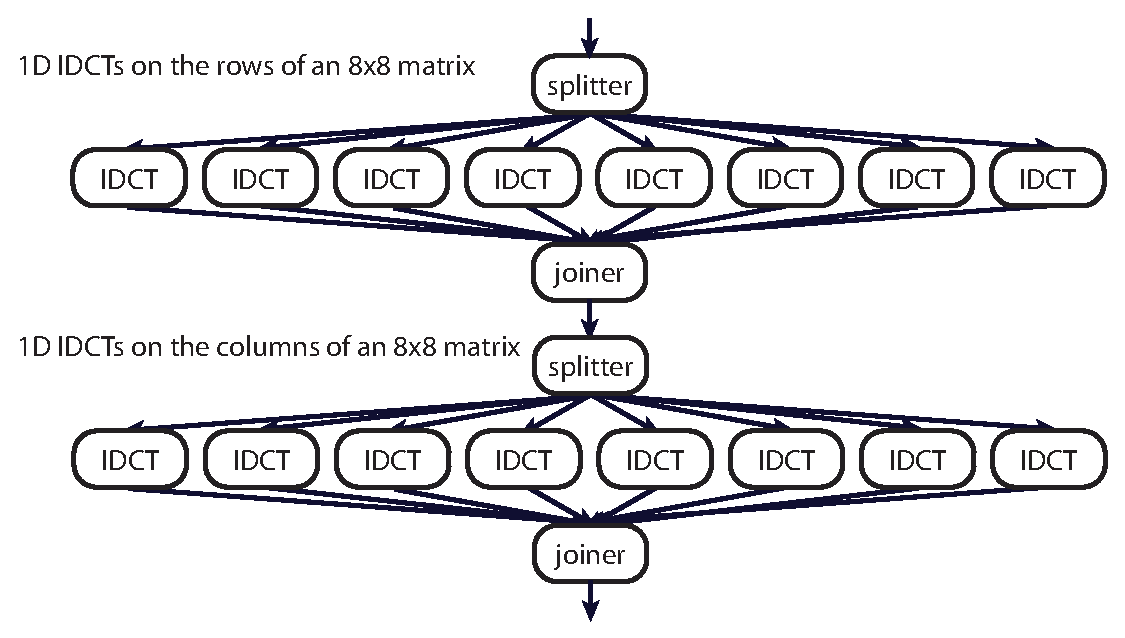
\includegraphics[scale=0.6, angle=0]{./dct_block.eps}
    \caption{Subgraph for a fine grained 2D inverse DCT.}
    \label{fig:decoder-sj-graph}
  \end{center}
\end{figure}

\begin{figure}[h]
  \begin{center}
    \begin{minipage}{4in}
      \begin{small}
        \begin{verbatim}
float->float pipeline IDCT_2D(int N) {
    // perform N 1D-IDCTs in parallel in the X direction
    add splitjoin {
        split roundrobin(N);
        for (int i = 0; i < N; i++)
            add IDCT_1D(N);
        join roundrobin(N);
    }
    // perform N 1D-IDCTs in parallel in the Y direction
    add splitjoin {
        split roundrobin(1);
        for (int i = 0; i < N; i++)
            add IDCT_1D(N);
        join roundrobin(1);
    }
}

float->float filter IDCT_1D(int N) {
    float[N][N] coeff = { ... };
       
    work pop N push N {
        for (int x = 0; x < N; x++) {
            float product = 0;
            for (int u = 0; u < N; u++)
                product += coeff[x][u] * peek(u);
            push(product);
        }
        for (int x = 0; x < N; x++) pop();
    }
}
        \end{verbatim}
      \end{small}
    \end{minipage}
  \end{center}
  \caption{StreamIt code for the fine grained 2D inverse DCT subgraph.}
  \label{fig:decoder-sj}
\end{figure}

\begin{figure}[h]
  \begin{center}
    \begin{minipage}{4in}
      \begin{small}
        \begin{verbatim}
// global variable
float coeff[64] = { ... };
      
void IDCT_2D(float* block) {
    int i, j, u;
    float product;
    float tmp[64];
        
    // 1D DCT in X direction
    for (i = 0; i < 8; i++)
        for (j = 0; j < 8; j++) {
            product = 0;
            for (u = 0; u < 8; u++)
                product += coeff[u][j] * block[8*i + u];
            tmp[8*i + j] = product;
        }

    // 1D DCT in Y direction
    for (j = 0; j < 8; j++)
        for (i = 0; i < 8; i++) {
            product = 0;
            for (u = 0; u < 8; u++)
                product += coeff[u][i] * tmp[8*u + j];
            block[8*i + j] = product;
        }
}
        \end{verbatim}
      \end{small}
    \end{minipage}
  \end{center}
  \caption{C code for 2D inverse DCT calculation using two 1D transforms.}
  \label{fig:idct_creference}
\end{figure}

Hierarchical constructs provide a convenient and natural
way to represent parallel computation. 
Figure~\ref{fig:decoder-sj-graph} shows a parallel
implementation of the 2D IDCT using 1D IDCTs. This
implementation is both data parallel (within the rows and columns) and
pipeline parallel (between the rows and columns). 
The StreamIt code for this 2D IDCT appears in Figure~\ref{fig:decoder-sj}.
A straightforward C implementation of a computationally equivalent
IDCT is shown in Figure~\ref{fig:idct_creference}. Note that
the code structure is similar to the StreamIt version, although it does 
not explicitly expose the parallelism; the compiler must perform loop
and dependency analysis to enable parallelism.
The C code also requires explicit array index management, such as the 
expressions $\texttt{block[8*i+u]}$ and $\texttt{tmp[8*i+j]}$, which are
notably absent in the StreamIt code. 
The splitter and joiner in StreamIt free the programmer from
tedious indexing operations, which also enables the compiler to
understand and optimize the buffer management~\cite{sermulins05lctes}.
The StreamIt implementation is also parameterized such that it is
trivial to adjust the size of the IDCT.

\section{Parallelizing Motion Prediction}
\label{sec:parallelmotion}

Motion prediction, in both the decoder and encoder, represents a significant fraction of the 
computational effort, and is amenable to data parallelism. Because each block in a 
picture has an associated set of motion vectors, motion prediction filters 
express a block-level transformation, and predictions for blocks may be formed in 
parallel. However, the act of forming the prediction requires a filter have access to 
full reference pictures. A parallel implementation of motion prediction will either lead 
to redundant copies of the reference pictures or the necessity for motion prediction 
threads to share a global read only memory space where the reference pictures can be stored. 
A parallel motion prediction algorithm is easy to express in StreamIt and exposes the 
necessary information so that the compiler can provide a shared-memory storage for the 
reference pictures.

\begin{figure}[h]
  \begin{center}
    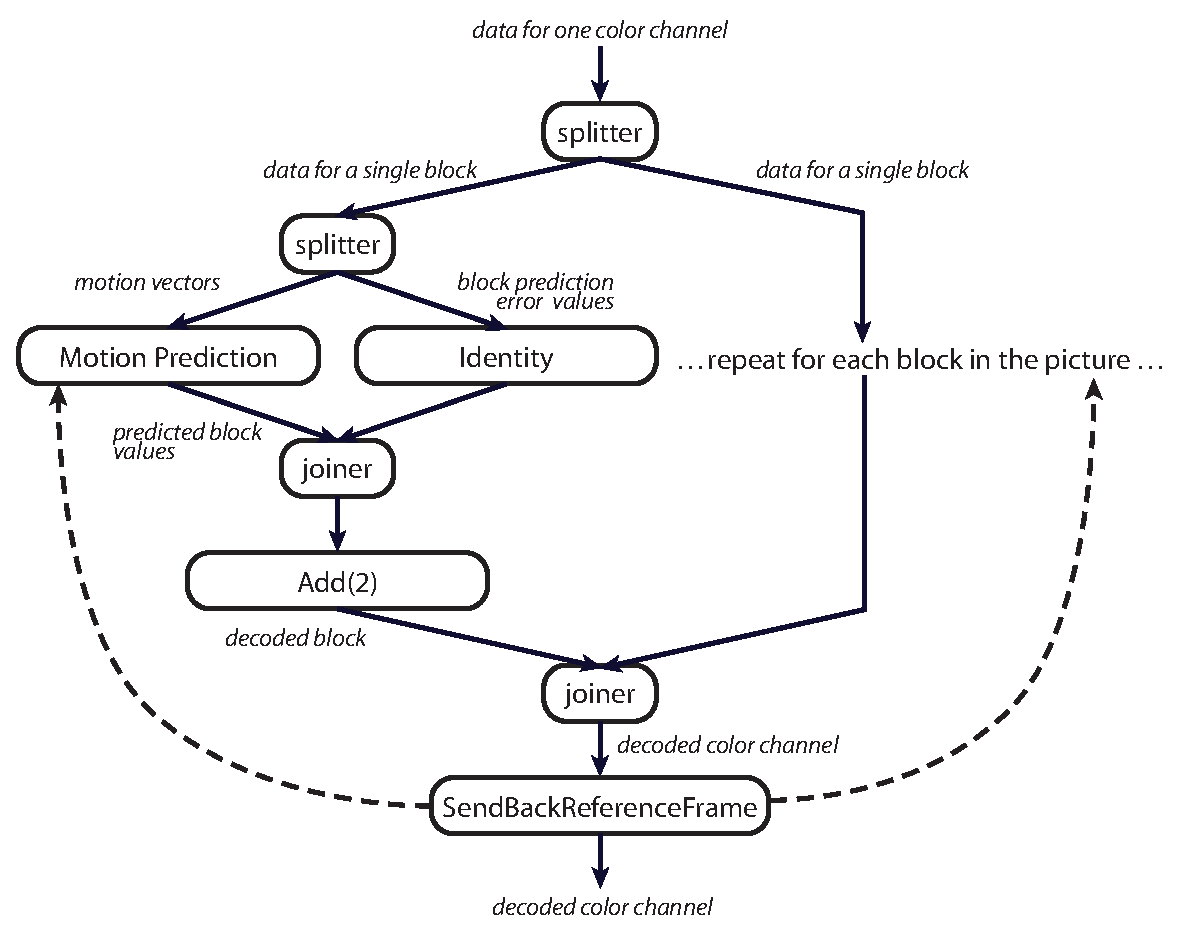
\includegraphics[scale=0.7, angle=0]{./motion_compensation.eps}
    \caption{Stream topology for motion compensation of a single color channel.}
    \label{fig:motion_prediction_parallel}
  \end{center}
\end{figure}

Figure~\ref{fig:motion_prediction_parallel} shows the StreamIt pipeline responsible for 
motion compensation of a single color channel in the decoder. All blocks in a given 
picture are motion predicted in parallel, with a set of block prediction error values 
and motion vector information sent to each motion prediction filter. Each data set then 
has its block coefficients (which need no processing) and the motion vectors splitup, 
sending the motion vectors to the filter that actually does the work of computing the 
predicted block using the motion vector offsets. The predicted block output is added 
to the block prediction error to form the original block, and all blocks are 
interleaved in the data streams. The final filter in the stream graph is responsible for 
communicating this fully decoded picture back to the motion prediction filters. It 
does this by sending upstream messages containing the reference picture data.

Note the cleanliness of this parallel implementation: 
a programmer could manually change the number of blocks 
decoded in parallel and similarly, the compiler can 
automatically fuse filter instances to match the target 
hardware. 
Note also that the reference pictures needed 
by the motion compensation filter and the picture type 
data needed by both the motion compensation and 
reference frame sending filters are naturally expressed using 
messaging. Finally, note that the motion compensation filters
only need to form predictions using their available reference
pictures and a separate filter can make sure they access
the correct references.

As mentioned previously, the one potential drawback of this
scheme would be if each instance of the motion prediction 
filter required its own instance of the reference picture 
data. However, a simple optimization allows the compiler to 
detect that these motion prediction filters only use these 
reference pictures in a read-only context and they may be 
stored in a global address space. Suppose that a filter 
receives a message containing a nugget of data $X$. If a 
compiler can detect that the filter never modifies $X$, 
it can place a copy in a shared memory space and give the 
filter a reference to $X$. Whenever a new message is 
received, it simply gives the filter a new reference to the 
data in a different part of the shared memory space. If 
a filter modifies $X$ or the compiler cannot detect 
that the filter uses $X$ immutably, it must give the 
filter a copy of the message in its own address space. Some 
kind of reference count or garbage collection mechanism 
must be associated with data stored in the global space 
so that the memory can be freed or reused once no filters 
can access the data.

The read-only analysis and associated space saving 
optimization can be performed by the compiler automatically. 
This enables program implementations to use a global 
reference space, even though the language need not provide 
this feature. I have tested a prototype of this optimization 
in the StreamIt Java library, where garbage collection is 
easily handled, and verified that it works.

\section{Improving Decoder Parallelization}
\label{section:super_parallel}

Most MPEG-2 decoder implementations make spatial decoding 
precede temporal decoding, but nothing in the specification 
or decoding algorithms require this. To achieve a higher degree of 
parallelization, one would want to generate the predictions for a 
block in parallel with the spatial interpretation of the block 
coefficients. This has been tried with success in a hardware based 
implementation~\cite{schneider99spec}. Only near the final output 
stage must the prediction and spatial data be summed and the output 
generated.

\begin{figure}
  \begin{center}
    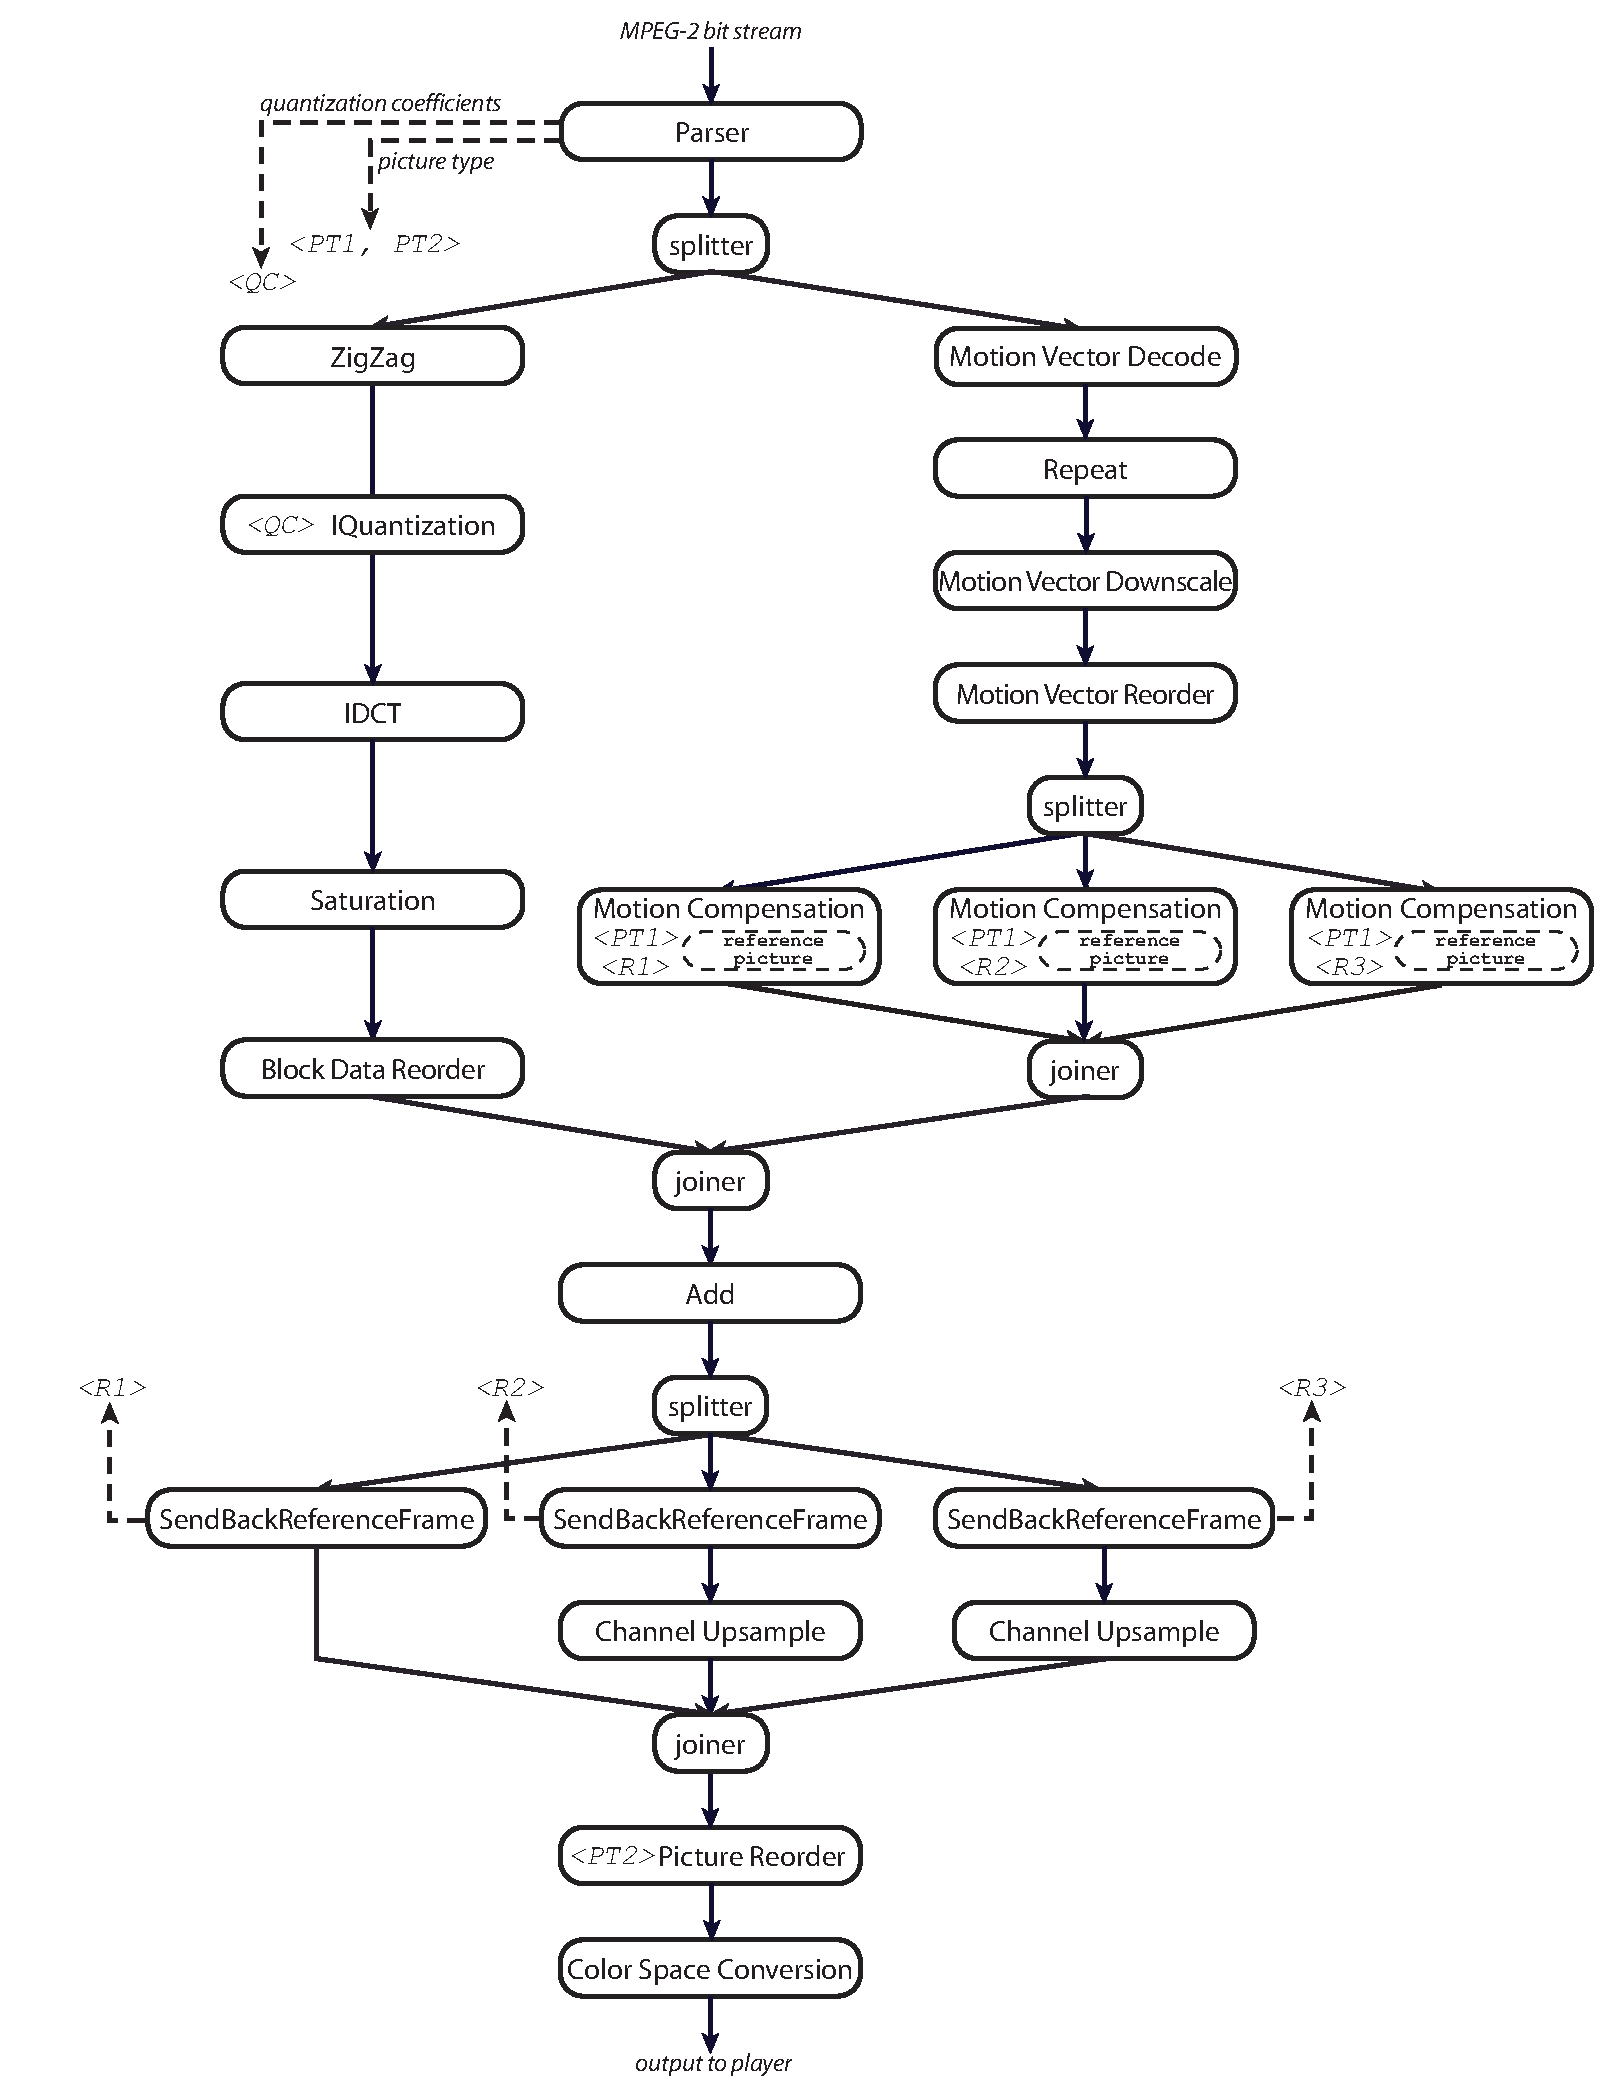
\includegraphics[scale=0.40, angle=0]{./decoder_total_parallelization.eps}
    \caption{Exposing parallelism between spatial and temporal decoding in an MPEG-2 decoder.}
    \label{fig:total_parallelization_vs_old_way}
  \end{center}
\end{figure}

I previously showed a block diagram for the MPEG-2 decoder 
in StreamIt (in Figure~\ref{fig:dec-with-code}). This diagram 
represents both a straightforward block specification and a program 
definition derived from the specification.  
Figure~\ref{fig:total_parallelization_vs_old_way} shows 
an alternative block diagram for an MPEG-2 decoder. This 
alternative diagram shows a block diagram that an MPEG-2 expert will decide 
upon\footnote{The original diagram represents the program structure 
I chose a month after originally familiarizing myself with the 
MPEG-2 specification. The new diagram represents the program 
structure I chose 8 months later after extensive familiarity 
with the specifications and implementations.}. These two block 
diagrams contain the same functional transformations. For an 
ideal language, a clean and malleable implementation of the 
original block specification in Figure~\ref{fig:dec-with-code} 
could easily be modified to expose the greater degree of 
parallelism present in the expert's block structure in 
Figure~\ref{fig:total_parallelization_vs_old_way}.

Because StreamIt preserves block structure in the program 
definition this transformation is easily accomplished. I have 
implemented the alternate decoder, using exactly the same 
filters as those used in the original decoder implementation. 
These two implementations are functionally equivalent, 
generating the same output across test cases. The only 
changes in the code are to the nested hierarchical container 
topologies that dictate the decoder stream graph. The ease 
with which a programmer can expose greater parallelism by 
merely changing the stream topology points to the 
usefulness of stream based languages for parallel program 
implementations.

\section{Performance Results}

This section provides performance results showing how StreamIt 
enables a compiler to provide scalable performance on MPEG-2 
codec implementations. A need for new language features previously 
mentioned in this thesis prevents the compilation of a full 
decoder or encoder\footnote{An intermediate Java library output 
from the compiler allows me to verify correctness of StreamIt code. This target is 
not performance oriented.}. 
Execution and evaluation of the complete MPEG-2 decoder and encoder stream graphs 
is a current focus of the StreamIt group.
Here I consider the spatial decoding subgraph, 
which represents up to a third of the total computation
in the decoder~\cite{iwata98coarse}.
I have extracted the 
spatial decoding code from the StreamIt and C decoder implementations
so that it can be compiled and run on a performance oriented target.

\begin{figure}[h]
 \begin{center}
  \begin{tabular}{|l|c|c|}
\hline
Granularity & Nodes in IDCT & Nodes in Graph\\
\hline
Coarse & 2 & 8 \\
Intermediate & 11 & 17\\
Fine & 20 & 26\\
\hline
  \end{tabular}
  \end{center}
 \caption{Three versions of the spatial decoding stream graph and their granularities.}
 \label{table:decoding_graphs}
\end{figure}

I use three versions of the StreamIt spatial decoding stream graph with
differing granularities. The granularities are changed by altering the subgraph
for the 8x8 IDCT. Figure~\ref{table:decoding_graphs} lists the number of nodes
(filters, splitters, and joiners), contained in the stream graph for each
of the three versions.
Each version contains \texttt{Source}, \texttt{ZigZag}, 
\texttt{InverseQuantization}, \texttt{Saturation}, \texttt{MismatchControl}, and
\texttt{Sink} filters. The coarse grained IDCT uses 2 filters for the IDCT: 
a \texttt{Rows\_iDCT} and a \texttt{Columns\_iDCT} filter. The fine grained
IDCT is expressed with 16 1D IDCTs and two splitjoins as described 
in Section~\ref{sec:2d_dct}. 
The intermediate IDCT uses the coarse \texttt{Rows\_iDCT} filter for the row
transformation and the fine grained column transformation with 8 1D IDCTs.

The performance evaluation is carried out on the Raw architecture
\cite{taylor:micro:2002, taylor:isca:2004}.
The Raw architecture is representative of the industry shift to multicore
embedded architectures, currently manifested in emerging architectures
such as the Intel Duo, AMD Opteron, and IBM Cell processors.
Raw is a wire-exposed multicore architecture which contains a 2D array of identical,
programmable tiles 
and supports instruction, data, thread, and pipeline parallelism. 
Each tile has a compute processor and a switch processor that
manages communication. The compute processor is composed of an eight-stage
in-order single-issue MIPS-style processor, a four-stage pipelined floating point unit,
a 32kB data cache, and a 32kB instruction cache. 
Tiles are connected by a FIFO queue 
with a 3 cycle near neighbor latency. This interconnect
network provides a mechanism for filters to communicate quickly with each other.
The current Raw prototype is a chip with 16 tiles running at 425Mhz. 
For this thesis, results are gathered using
a cycle-accurate simulator~\cite{taylor:isca:2004} that can model tile configurations
with size
1, 4 (2x2 grid), and 16 (4x4 grid). 

\begin{figure}[p]
  \begin{center}
    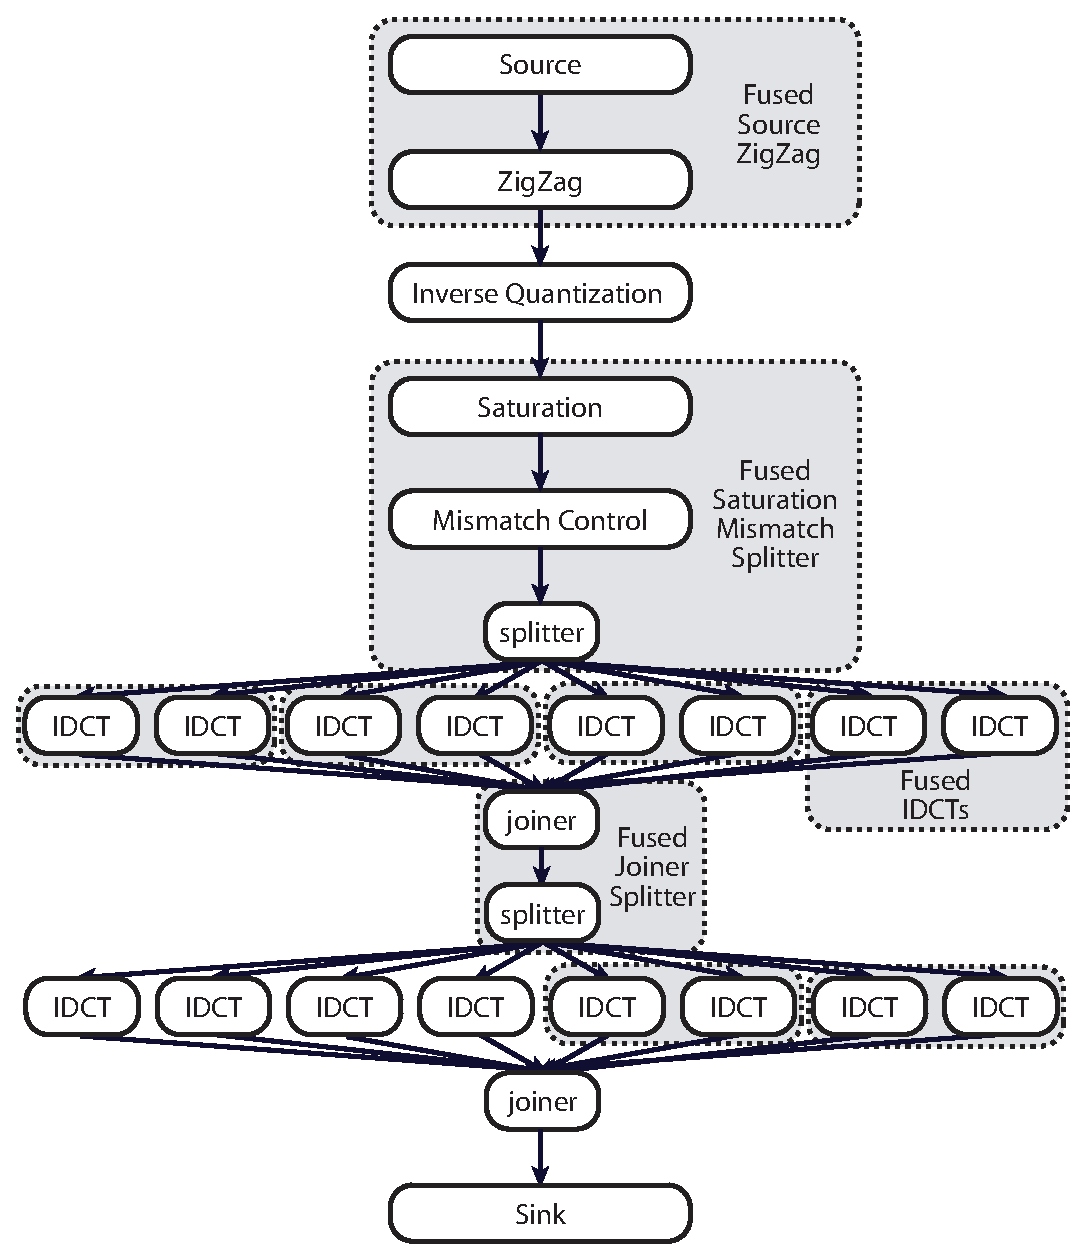
\includegraphics[scale=0.5, angle=0]{./partition.eps}
    \caption{Partitioning the spatial decoding stream graph for 16 tiles of Raw.}
    \label{fig:partition}
  \end{center}
\end{figure}

\begin{figure}[p]
  \begin{center}
    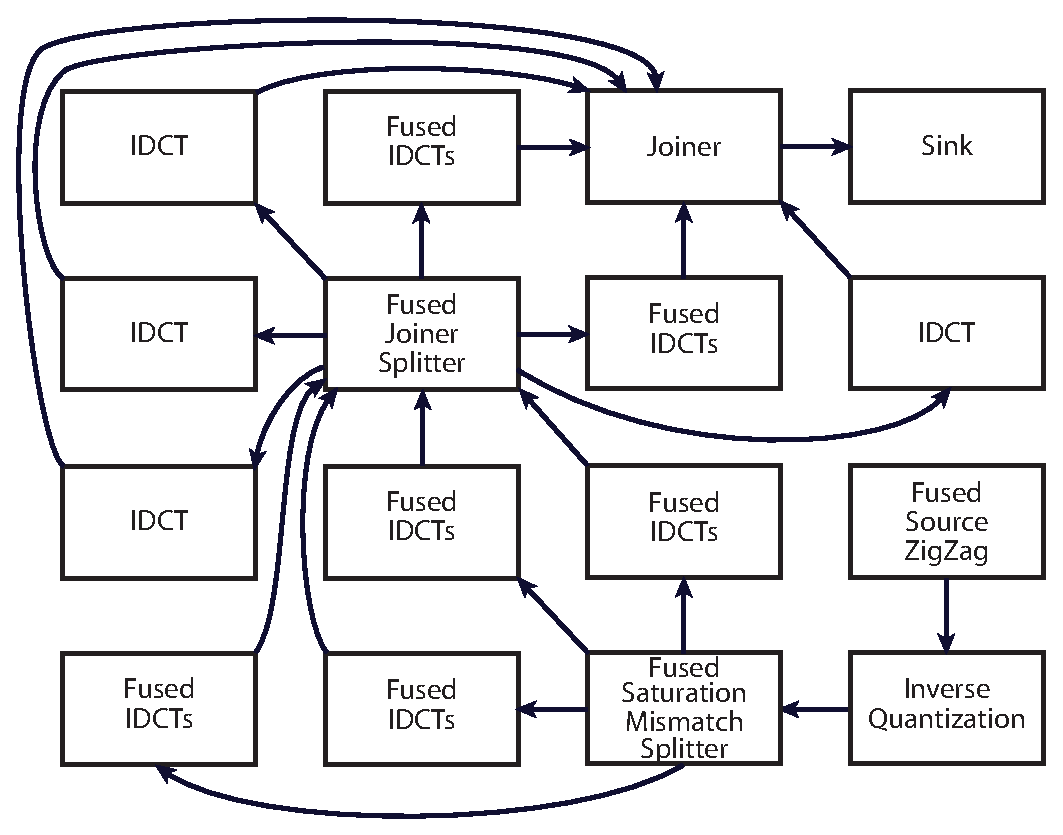
\includegraphics[scale=0.5, angle=0]{./layout.eps}
    \caption{Layout of the fine grained spatial decoding stream graph on the Raw chip.}
    \label{fig:layout}
  \end{center}
\end{figure}

The StreamIt code was compiled to Raw with the StreamIt 
space multiplexing compiler
\footnote{This compiler will soon be
deprecated in favor of a more advanced space-time multiplexing
compiler described in an upcoming paper~\cite{gordon06asplos} 
from the StreamIt group.}
described in~\cite{gordon02asplos}.
The code was compiled at an \texttt{-O1} optimization level, 
which performs loop unrolling by a factor
of 16, scalar replacement, and aggressive constant propagation. 
The StreamIt compiler focusses on achieving
performance by enabling scalable execution on
many tiles. Using the parallelism explicit in the stream graph the compiler
automatically performs task partitioning and layout.
An application should achieve significant speedups as the number of tiles increases.

A brief example illustrating
scheduling and layout follows.
Figure~\ref{fig:partition} shows how the StreamIt
compiler partitions the fine grained 
spatial decoding stream graph for a Raw configuration with 16 tiles.
The compiler adjusts the stream graph granularity by combining
nodes to eliminate buffering between nodes on the same tile. 
The dotted lines in the figure show which nodes in the stream graph have been fused.
After fusion is complete there are the same number of nodes and tiles 
in the stream graph. Figure~\ref{fig:layout}
shows the compiler's layout decision for these nodes on the Raw hardware.

\begin{figure}[t]
  \begin{center}
    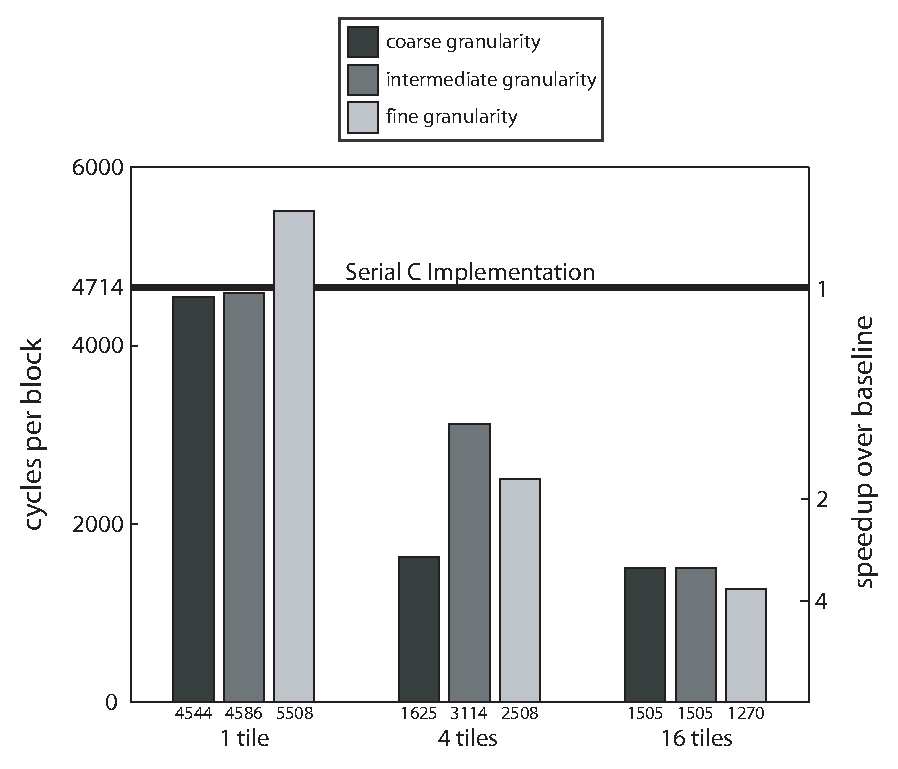
\includegraphics[scale=0.7, angle=0]{./performance_graph.eps}
    \caption{Scalability of StreamIt spatial decoding pipeline against single tile C baseline.}
    \label{fig:performance_results}
  \end{center}
\end{figure}

Figure~\ref{fig:performance_results} shows results for execution of 
the spatial decoding stream graph at three granularities.
The baseline is
the C reference code running on a single tile. 
The C code was compiled with a Raw port of the \texttt{gcc} compiler,
which performs register allocation and list scheduling.
A compiler has a difficult time extracting parallelism from single threaded C code
(hence the need for new programming models); in StreamIt the parallelism
is explicit, so we show performance numbers for multi-tile 
configurations as well. 

Single tile StreamIt performance is roughly equivalent to the
single tile C code. Small variations are explained
by compiler decisions about how to fuse all the filters together. 
When the tile size increases to 4, all versions of the StreamIt
code significantly outperform the C implementation. While 
the coarse grained
version of the StreamIt code outperforms the more fine grained
implementations, an analysis of the compiler's layout decisions suggests
that this result is somewhat anomalous: the compiler is 
getting exceptionally lucky with load balancing. The intermediate
and fine grained versions are more prototypical.
At 16 tiles performance of all stream graphs 
again improves significantly. One 
sees the general trend that decreasing the granularity of
the program enables the compiler to make better layout
decisions and provide higher parallel performance. The best 
performance comes from a fine-grained implementation 
operating on 16 tiles.

\chapter{StreamIt Limitations and Proposed Extensions}
\label{section:impl_issues}

During the implementation process I encountered situations 
 where StreamIt forced a poor expression of a computation or 
language features did not scale for large application development. 
A language design oriented to small applications and benchmarks could easily 
miss these pragmatic development issues. The StreamIt group has focussed on 
these issues; 
the next version of StreamIt will add a number of language
extensions that improve programmability, modularity, 
and expression of parallelism and 
communication. 
This chapter provides concrete 
examples motivating
the introduction of these features and attempts to steer the direction of 
future streaming languages.

\section{Bitstream Parsing}

In MPEG-2, the process of parsing the bitstream and performing Huffman 
and run-length coding is estimated to constitute almost a third 
of the computational effort~\cite{iwata98coarse}. Unfortunately, many 
layers of nested control flow make the parser unsuitable for streaming 
computation. The parser must be implemented as a single filter that 
contains approximately one thousand lines of code, almost half the code 
lines in either the decoder or encoder. This filter expresses scheduling 
information and parallelism poorly. 

Filters with dynamic IO rates present particular difficulties for the 
StreamIt compiler because of the lack of scheduling information. However, 
certain filters are naturally expressed by the programmer with dynamic 
input and output rates, although they theoretically could 
be realized with static rates. 
In the decoder, the parser has a dynamic 
input rate, but always outputs full macroblocks, and ought to be expressed 
with a static output rate. (The reverse is true for the parser in the encoder.) 
However, due to the complexity of the MPEG-2 bitstream format, the actual 
push statements are embedded in deeply nested control flow. The parser is 
most naturally expressed in terms of a single work function execution 
that parses the entire MPEG-2 bitstream. 

This presents several difficulties. The fact that the parser processes all 
its data in a single pass means that if the filter were to execute atomically 
with respect to other filters, one would need a potentially infinite buffer 
between the parser and the downstream graph. To avoid this difficulty the 
compiler would need to generate multi-threaded code, even for a uniprocessor 
backend, that interleaves the parser execution with downstream execution. 
Messaging presents a second difficulty.
A filter's messaging granularity is determined by its input and output rates, 
and messages are timed with respect to the work execution boundaries; a work 
function that processed an entire video in a single execution could only 
time messages with respect to the beginning or end of the video, not with 
respect to individual macroblocks within the video.

I present a workaround that allows for interleaved scheduling and message 
delivery. Given a filter with a large work function, such as the parser, 
one can move control flow determining variables into filter instance 
variables that are maintained between work function executions. Inside 
the work function invocation is a loop that repeatedly branches to one 
of several helper functions determined by the control variables. The 
helper functions update the control variables, and the loop terminates 
after executing any of the helper functions that generates output (for 
the parser, pushing a macroblock). This workaround amounts to replacing 
nested control flow with a flat control flow graph structure. The 
readability and malleability of the code suffers. 

Even with such a hack, parallelism is expressed poorly because the parser 
itself cannot be parallelized easily. Two constructs in the MPEG-2 bitstream 
facilitate parser parallelism. At the higher level, every GOP can be decoded 
in parallel, since pictures can only reference other pictures in the same 
GOP. At a lower level slices may be decoded in parallel since macroblocks 
contained inside different slices in a picture are known to have no 
interdependencies. The codes for the start of a GOP or slice are 
byte-aligned and never occur in any other context. A parser exploiting
thread-level parallelism 
could first scan through a bitstream and identify the GOP and slice 
structures, and then subdivide portions of the bitstream to different 
bitstream parsers. Ahmad et al. show this technique to be 
effective for parallelizing MPEG-2~\cite{ahmadmpeg2encoder3}. 
This sort of parser parallelization is difficult to 
express in a stream based language and achieving reasonable performance 
would require a Herculean compiler effort.

The StreamIt group has considered language features to address these 
problems, but our key insight is the realization that StreamIt targets 
streaming computations, and if a filter cannot concisely express a 
computation then that computation is probably not streaming. For the MPEG-2 
parser this is obvious because its expression requires a thousand line 
functional block and leaves the compiler with an intractable parallelism 
problem. MPEG-2 bitstream parsing has little in common with stream 
computation and much in common with context-free grammars, and would be 
implemented more easily in a language like C. Clean interfaces between 
StreamIt and traditional languages, under development in the StreamIt 
language group, would allow hybrid language compression scheme implementations 
that share the benefits of both languages. MPEG-2 provides a strong motivation
for such a hybrid; while the majority of MPEG-2 coding is particularly well 
suited to a streaming approach, bitstream parsing is an important exception 
that demands an alternate approach.

\section{Functions with Tape Access}

Functions provide an abstraction that improves programmability when a computation 
must be repeated within a single work execution of a filter. Support for arbitrary 
tape accessing functions is a current focus of the StreamIt compiler group. A 
scheduler can handle both external and helper functions with tape access; the 
overall work rate of a filter should reflect any tape access caused by functions 
it calls. This section gives examples showing this feature's importance. 

\paragraph{External Functions with Tape Access}

\begin{figure}
  \begin{footnotesize} 
  \begin{center}
  \begin{minipage}{4.7in}
    \setlength{\columnseprule}{1pt}
    \begin{multicols}{2}
     \begin{minipage}{3in}
      \begin{verbatim}
...
int horizontal_size_value = 
  popbits(12);



int vertical_size_value = 
  popbits(12);



int aspect_ratio_information = 
  popbits(4);



int frame_rate_code = 
  popbits(4);



...
      \end{verbatim}
     \end{minipage} 

     \begin{minipage}{4in}
      \begin{verbatim}
 ...
 int horizontal_size_value = 0;
 for (int i = 0; i < 12; i++) {
   horizontal_size_value <<= 1;
   horizontal_size_value += pop();
 }
 int vertical_size_value = 0;
 for (int i = 0; i < 12; i++) {
   vertical_size_value <<= 1;
   vertical_size_value += pop();
 }
 int aspect_ratio_information = 0;
 for (int i = 0; i < 4; i++) {
   aspect_ratio_information += pop();
   aspect_ratio_information <<= 1;
 }
 int frame_rate_code = 0;
 for (int i = 0; i < 4; i++) {
   frame_rate_code <<= 1;
   frame_rate_code += pop();
 }
 ...
        \end{verbatim}
     \end{minipage}
    \end{multicols}
  \end{minipage}
  \end{center}
  \end{footnotesize}

  \caption{Code fragment from parser with (left) and without (right) tape accessing external functions.}
  \label{fig:mpegbitpopexample}
\end{figure}

Data compression formats such as JPEG and MPEG-2 pack data together as 
tightly as possible, ignoring word and byte boundaries in a data stream 
except for certain byte-aligned \textbf{escape codes} used to help a parser 
detect its position in a data stream. Even uncompressed formats, such as 
BMP~\cite{bmp} pack some configuration data. 
Parsers need functions that allow them to specify that a sequence of $N$ 
bits appearing in the bitstream should be consumed and stored as some data 
type, such as an integer. The left half of Figure~\ref{fig:mpegbitpopexample} 
shows example 
code from an MPEG-2 parser with external functions. The alternative approach 
without external functions appears in the right 
half\footnote{The particular ability to pop, 
push, and peek multiple bits at a time from (or to) bitstreams, as 
illustrated in this example, is needed so frequently that all of the 
implementations described in this paper assume that these global functions 
exist and must be preprocessed before being sent to the StreamIt compiler.}.

\paragraph{Helper Functions with Tape Access}
\label{sec:helperfunctionswithtapeaccess}
Helper functions with tape access allow for cleaner code. 
They differ primarily from external functions with tape access 
in that they would be private to the filter that contains them
and could manipulate internal state within that filter. 
The work function from the filter responsible for motion prediction
is 103 lines and is difficult to read or edit (the code is omitted due to length).
With tape-accessing helper functions it would decompose nicely into a work
function and three helper functions, each of 20 to 30 lines.

\section{Messaging Interfaces}
 
In the current version of StreamIt, a filter {\tt X} declares the types of messages 
it receives, and an associated {\tt portal<X>} is implicitly declared. Only filters 
of the same type may subscribe to the same portal, so redundant portals must be 
declared if different parts of a computation need the same sets of messages. The 
StreamIt group has recognized this limitation and the upcoming language revision 
will introduce messaging interfaces, conceptually similar to Java's interface 
declaration, that decouple portal specifications from subscriber implementations. 
An interface declares a set of valid messages, and any filter which implements the 
interface may subscribe to portals of the interface's type. 

Separating portal and subscriber definitions removes the dependency that senders 
broadcasting messages to a portal of type {\tt portal<X>} have on subscribers 
that implement \texttt{X}. This dependency limits the expression of large applications 
and I provide empirical evidence that motivates implementation efforts for this feature. 
Consider again 
Tables~\ref{table:enumerate_messages_decoder}~and~\ref{table:enumerate_messages_encoder}. 
The number of distinct message subscriber types demonstrates the need for interfaces.
Without interfaces, one must write each message sender after implementing all of its 
message receivers. In the encoder, enough components exchange information about picture 
and block metadata that message passing without interfaces became unmanageable and many 
parameters were embedded in the data stream. Interfaces enable one to write an MPEG-2 
bitstream parser before writing --- or even determining --- the many downstream 
components that will need to receive control parameters from the parser. 

\section{Programmable Splitjoins}
\label{sec:program_splitjoins}

The current language semantics support roundrobin and duplicate splitters, and roundrobin 
joiners. Roundrobin components need not send or receive identical amounts on each of their 
substreams, but the rates must be statically determined. Some applications require 
computations which dynamically switch between several modes of computation based on data. 
Messaging can address the issue when the modes of computation are very similar. However, 
in cases where the computations differ significantly, it would be more natural to place 
independent filters in parallel and have a splitter select one of the filters for each 
set of data to be processed. This provides a need for programmable splitters and joiners 
which can receive messages that determine the data streams to which they should output. 
I first give an example where some kind of \textbf{switch} splitter that sends to one of 
its channels would suffice, and then show a case where programmable splitters and joiners 
are needed.

\paragraph{Switch Splitjoins}

\begin{figure}[t]
  \begin{center}
    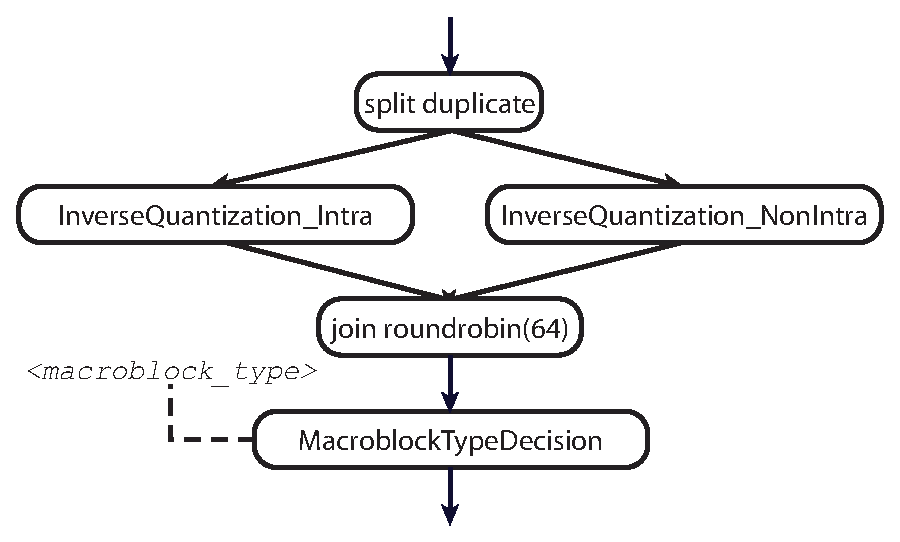
\includegraphics[scale=0.5, angle=0]{./inverse_quantization.eps}
    \caption{Inverse quantization subgraph with a duplicate splitter and roundrobin joiner.}
    \label{fig:inversequant}
  \end{center}
\end{figure}

\begin{figure}[t]
  \begin{center}
    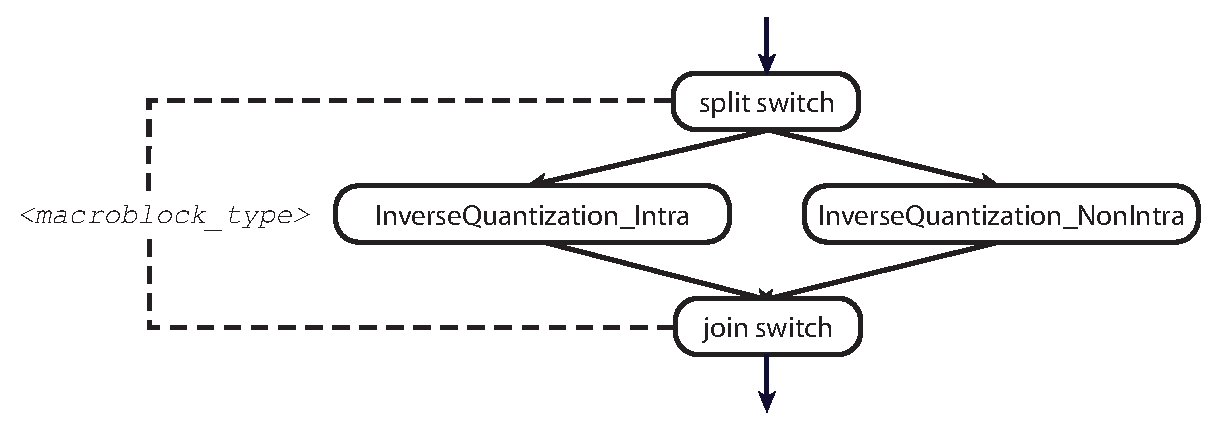
\includegraphics[scale=0.5, angle=0]{./inverse_quantization_switch.eps}
    \caption{Inverse quantization subgraph with switch splitters and joiners.}
    \label{fig:inversequant_switch}
  \end{center}
\end{figure}

Figure~\ref{fig:inversequant} shows the inverse quantization subgraph as it is realized in the 
MPEG-2 decoder. The inverse quantization process uses two different transforms depending on whether 
a block is intra coded or residually coded. The current implementation uses a splitjoin to 
duplicate each quantized block and process it for both block types. The results are interleaved 
and a downstream filter takes in both results and outputs one of them. Messages to the decision 
making filter from the upstream parser control which result gets output.

This approach results in needless computation since only one of the two intermediate filters 
needs to execute. Dataflow is also complicated by the interleaving and filtering of data. 
In this case, a paired switch splitter and joiner are desirable. The idea is that a switch 
splitter and joiner with coordinated behavior would receive messages which cause them to 
change which channel processes the data. Figure~\ref{fig:inversequant_switch} shows how the 
subgraph would appear with a switch splitter and joiner.

\paragraph{User Programmable Splitters}

Motion estimation in an MPEG-2 encoder, previously described in 
Section~\ref{encoder:estimation}, illustrates the need for a programmable splitjoin. As implemented 
in Figure~\ref{fig:motion_estimation_subgraph}, a duplicate splitter sends data to each of the 
compression filters. A roundrobin joiner interleaves each of the compression results and sends 
them to a downstream filter which determines the best encoding technique and emits only one of 
the compression results. However, this results in extra work. For I pictures one need not try 
motion estimation and for P pictures one need not try backward motion prediction. With only 
duplicate splitters and roundrobin joiners one is forced to send and receive data from the unneeded 
compression filters and then discard the results.

In an ideal implementation, the splitter and joiner would be 
programmable and messages about picture type would dictate which, 
and how many, internal streams processed the data. 
Figure~\ref{fig:motion_estimation_subgraph2} illustrates a stream 
graph with this form. A switch splitter will not suffice because 
multiple streams within the splitjoin must receive the input in 
certain cases. The joiner is also the ideal place to make the 
decision about which candidate blocks are used. For any given picture type, 
it must pop off the candidates from the valid input lines and output 
the one that exhibits the best compression. Note that the 
programmable splitter and joiners for this subgraph will be dynamic rates.
However, the motion estimation subgraph is still static rate with respect
to the rest of the stream graph and has a well-defined internal schedule.
I explain how this scheduling information can be exposed to the 
compiler in the next section.

\begin{figure}[h]
  \begin{center}
    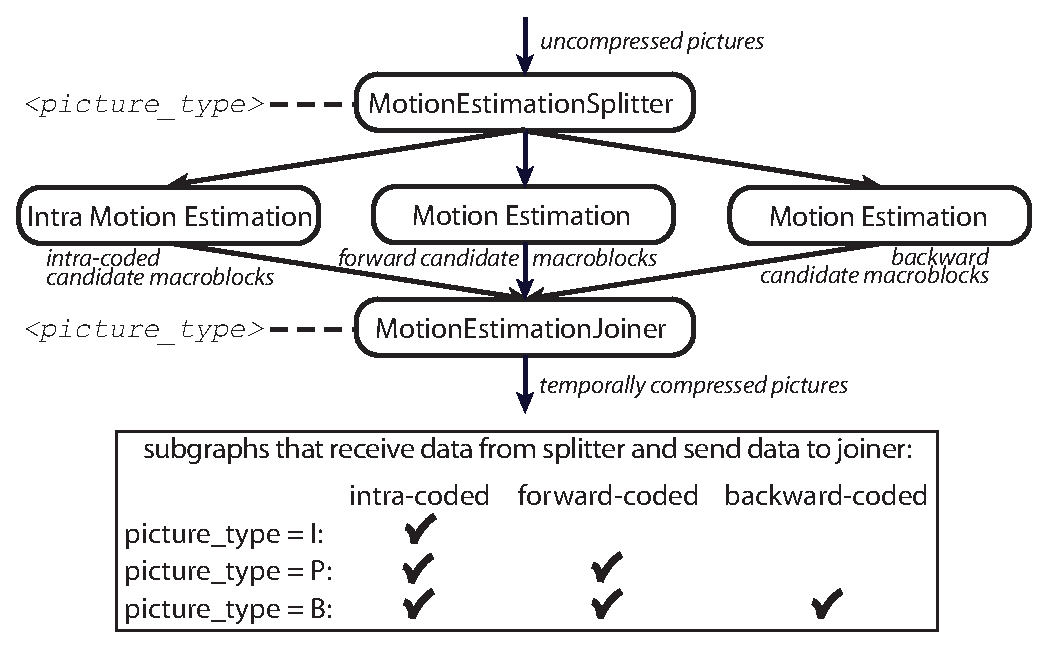
\includegraphics[scale=0.8, angle=0]{./motion_estimation_programmable.eps}
    \caption{Motion estimation stream subgraph with a programmable splitter and joiner.}
    \label{fig:motion_estimation_subgraph2}
  \end{center}
\end{figure}

Another part of the encoder that would benefit from programmable splitjoins
is the \texttt{ReferenceFrameHandler} responsible for decoding the 
recently encoded reference pictures and 
sending them upstream to the motion estimation filters. The subgraph
for this component appears in Figure~\ref{fig:referenceframe}.

\begin{figure}[h]
  \begin{center}
    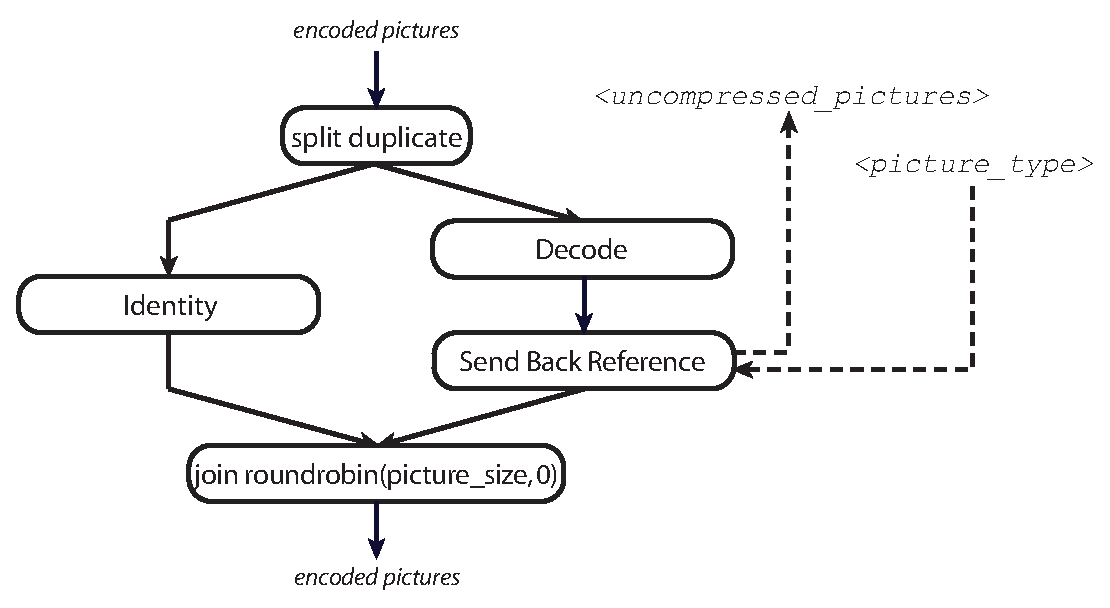
\includegraphics[scale=0.6, angle=0]{./referenceframe.eps}
    \caption{Subgraph for decoding reference pictures and sending them upstream.}
    \label{fig:referenceframe}
  \end{center}
\end{figure}

As currently realized, both reference pictures and non-reference pictures
go to a duplicate splitter. One duplicate of the encoded picture passes back 
to the joiner unchanged, and the other goes to a subgraph that first
decodes the picture and then sends it as an upstream message
to the motion estimation filters. The subgraph for decoding the picture
looks similar to the MPEG-2 decoder pipeline.

One problem with this behavior is that the filter responsible for messaging
back the reference frame must determine whether or not to send the 
picture or merely discard it, based on the picture type. This is
problematic because many pictures are discarded, yet they are still properly
decoded. A programmable splitter 
could receive picture type messages and selectively send only the 
reference frames to the decoding subgraph. This would avoid
unnecessary computation.

\section{Named Work Functions}

Many filters whose work function behavior is dependent on stream parameters 
have a similar implementation pattern: state variables are declared and are 
used as parameters or control flow indicators in the work function, and only 
ever modified in message updates. 

A more intuitive mechanism for the programmer 
would be to allow multiple named work functions or a single named work 
function that declares parameters (like a function or filter 
declaration). These named work functions would act as message receivers, and 
other portals could directly call the work functions through the teleport 
messaging mechanism. 

From a sending filter's standpoint, messaging is unaffected.
Whether a receiver implements a message handler as a 
named work function or a message handler is irrelevant to the messaging semantics. 
When a filter with a named work function receives a message, 
it would change the filter's mode of execution to the named work function,
using the work function parameters if they exist.

Using named work functions simplifies the programming of the quantization, motion 
estimation, and picture reordering filters in the encoder, and the inverse 
quantization and motion prediction filters in the decoder. 
This feature also makes filter behavior more transparent to the compiler
by exposing scheduling information about otherwise dynamic rate components. 
For instance, some dynamic rate filters could be declared as static rate filters
if the different named work functions had different pop and push rates.

As an example, I consider the MPEG-2 encoder's motion estimation 
subgraph realized using programmable splitters and joiners, previously
described in Section~\ref{sec:program_splitjoins}. As 
Figure~\ref{fig:motion_estimation_subgraph} points out, the splitter
and joiner will need to have different IO rates depending on the 
picture type, because different numbers of the splitjoins
internal streams may need to receive picture data.
With dynamic splitter and joiner IO rates, a compiler would be unable to 
intelligently schedule the subgraph's execution.

Suppose the splitter and joiner could each be implemented using 
three named work functions. Each work function would have a different but
static rate declaration. By sharing the same interface and subscribing
to the same message portal, this would expose the scheduling information
to the compiler, which could realize that the splitjoin viewed as a whole
has a static IO rate with respect to the rest of the graph. 

\section{Stream Graph Reinitialization}

The biggest limitation of StreamIt 2.0 codec implementations
is a requirement placed on video and image parameters that determine 
stream graph topology. These parameters must be declared at compile-time. 
Image size and chroma format must be hardcoded and changes to these values 
require that the source code be modified and the program recompiled. 
This limitation can be removed by allowing portions of a stream graph 
to reinitialize at runtime. Others have had success allowing actors to
reinitialize at runtime and change their internal 
state~\cite{neuendorffer04hierarchical}, and it should be possible
to allow topology changes at runtime as well. I believe this language
feature is necessary  and the StreamIt group is introducing the ability
in StreamIt 3.0.

\section{Stream Graph Draining}

The streaming model of computation assumes that input and output streams are infinite 
and actors will process continuously with a steady state behavior. However, real 
world applications such as MPEG-2 have definite stream endings, and the end of life 
behavior of a stream graph is poorly determined. The MPEG-2 decoder, for instance, 
needs to be \textit{drained} so that filters internally buffering data release their 
buffers. An example of this is the filter responsible for picture reordering 
(previously shown in Figure~\ref{fig:picture_reorder}) which buffers one reference frame 
internally. For this frame to get released, the current implementation requires that 
the first filter in the pipeline, after detecting its final input, send dummy data 
items through the pipeline to empty out the remaining buffers. However, this behavior 
is non-ideal because spatial and temporal decoding are performed on data whose only 
purpose is to cause the downstream filter to release buffered data items. Just as 
the \texttt{prework} keyword helps a stream-graph reach a steady-state behavior at 
application startup, a similar mechanism (e.g., \texttt{postwork}) is needed at the 
end of an application's lifetime.
\section{Conclusions}\label{ch:conc}

Streaming languages such as StreamIt provide an excellent way to target new multicore architectures while placing minimal parallelization burden on the programmer. The Cell architecture is designed to offer high peak performance, and is very suited for streaming applications. This thesis described a runtime framework for streaming applications on Cell consisting of \emph{i}) a runtime library that provides high-level primitives for schedulers and \emph{ii}) a dynamic scheduler for stream graphs. The framework greatly simplifies the task of a streaming language compiler or scheduler.

The real benefit provided by the framework, in particular the runtime library, is that it allows a scheduler to think directly in terms of filters and how they are scheduled instead of lower-level architecture-specific details. It requires far less code to implement scheduling patterns on top of the library than directly on Cell hardware, and the library also allows far more complex patterns to be implemented. The runtime library running the data-parallel fused FFT benchmark produces a reasonably small amount of overhead (1.2\%), and the dynamic scheduler running the pipelined version of the benchmark produces an acceptable amount of overhead (8.6\%).

\section{Future Work}

The runtime library currently provides two orthogonal branches that can be further developed. First, it is important to reduce the 9\% overhead observed in the pipelined FFT tests involving the dynamic scheduler. This overhead is entirely due to the cost of the run list when many commands are active, and it can probably be significantly reduced by optimizing library code, although it is also likely that doing so would make the SPE library implementation, especially the run list, much more specialized.

In addition, the library currently lacks real support for filters with dynamic rates -- the library simply leaves the responsibility of tracking rates to the scheduler entirely. Feedback from the library on how much data filters have produced and consumed would be very useful for schedulers; ultimately, the library should have some way of running filters with unbounded dynamic rates. The latter would require a general mechanism to suspend dynamic rate filters in the middle of executing their work functions.

The dynamic scheduler can be extended in many directions. The simplest additions involve adjusting the metric used for selecting filters to test and improve the performance of the dynamic scheduler as work becomes more and more imbalanced between filters. In addition, an important advantage of dynamic scheduling in general is the ability to react to dynamic rate filters and the runtime distribution of work in the stream graph; implementing robust support for dynamic rate filters in the stream graph would drastically increase its usefulness.


%% This defines the bibliography file (main.bib) and the bibliography style.
%% If you want to create a bibliography file by hand, change the contents of
%% this file to a `thebibliography' environment.  For more information 
%% see section 4.3 of the LaTeX manual.

\bibliography{main}
\bibliographystyle{plain}


%% ALWAYSCHECK - all figs and citations match, all sections match, all references match
%% ALWAYSCHECK - MPEG and StreamIt terms first encountered - bold or italics? make sure it's consistent everywhere
%% ALWAYSCHECK - correct grammar (naked this, which/that, etc)
%% ALWAYSCHECK - compensation vs estimation vs prediction

\end{document}

